\documentclass[a4paper,12pt,oneside,onecolumn,final,fleqn]{repUERJ}

% ---
% OBRIGATÓRIO
% Pacotes fundamentais 
% ---
\usepackage[brazilian]{babel}    % adequação para o português Brasil
\usepackage[utf8]{inputenc}   % Determina a codificação utilizada
\DeclareUnicodeCharacter{2208}{\ensuremath{\in}}
                              % (conversão automática dos acentos)
\usepackage[T1]{fontenc}
\usepackage{indentfirst}      % Indenta o primeiro paragrafo de
                              % cada seção.
\usepackage{graphicx}         % Inclusão de gráficos
\usepackage{subfig}
\usepackage{multirow}
\usepackage{amsmath,amssymb}  % pacotes matemáticos
\usepackage[maxfloats=25]{morefloats}

\usepackage{makeidx}                % Cria o índice

\usepackage[hyphens]{url}
\usepackage[pagebackref]{hyperref}  % Controla a formação dos hyperlinks
\makeatletter
\pdfstringdefDisableCommands{\let\uline\relax}
\makeatother
\hfuzz=20pt
\vfuzz=20pt
\hbadness=10000
\vbadness=10000
\AtBeginDocument{\hfuzz=20pt\vfuzz=20pt\hbadness=10000\vbadness=10000}

% ----------------------------------------------------------------
% OBRIGATÓRIO 
% ----------------------------------------------------------------
% para referências no estilo autor-data (recomendado pela ABNT)
% ----------------------------------------------------------------
\usepackage[alf]{abntex2cite} % pacote para citacoes autor-data
% ----------------------------------------------------------------

% ----------------------------------------------------------------
% OBRIGATÓRIO: repUERJformat
% * Estilo que implementa os comandos principais do pacote repUERJ
%   pacote para as normas da UERJ
%       font=default
%           --> Fontes tipográficas
%          font=default  : fonte computer roman (latex) : remomendado
%          font=times    : fonte times new roman (próximo da fonte MS)
%          font=sans     : fonte sans (helvética)
%          font=lmodern  : fonte sans (próximo Adobe Arial)
%          font=palatino : fonte serif palatino
%
%       frame=no
%           --> Grade de margeamento do texto
%           frame=yes : ativa exibição da moldura
%           frame=no  : desativa exibição da moldura (recomendado)
%
%       backref=yes
%           --> Hiperlink retroativo das citações na Referência
%               para simples conferência
%           backref=yes : citação retroativa ativada
%           backref=no  : citação retroativa desativada (recomendado)
%
%       ilustrations=yes
%           --> Controla a geração da lista de ilustrações:
%           ilustrations=yes : lista única de ilustrações
%               permite gerar
%                   LISTA DE ILUSTRAÇÕES: juntos: figuras, quadros e gráficos
%           ilustrations=no  : listas separadas
%               permite gerar
%                   LISTA DE FIGURAS: somente figuras
%                   LISTA DE QUADROS: somente quadros
%                   LISTA DE GRÁFICOS: somente gráficos
%
% ----------------------------------------------------------------
\usepackage[font=default,frame=no,backref=no,ilustrations=yes]{repUERJformat} 

\usepackage[dots=yes,num=yes]{repUERJpseudocode}

\usepackage{xwatermark}


% ----------------------------------------------------------------
% ----------------------------------------------------------------
% FIM DO PREÂMBULO DO DOCUMENTO (preamble latex documento)
% ----------------------------------------------------------------
% ----------------------------------------------------------------

% ----------------------------------------------------------------
% OPCIONAL
% verbatim para os campos do bibtex 
% configura a apresentação dos exemplos
% ----------------------------------------------------------------

\usepackage{framed,color,verbatim}
\definecolor{shadecolor}{rgb}{.9, .9, .9}
\newenvironment{vrbcode}%
   {\snugshade\verbatim}%
   {\endverbatim\endsnugshade}

\newcommand{\cmd}[1]{\noindent\texttt{\textbackslash #1}}
\newcommand{\opc}[1]{\texttt{\{#1\}}}

\newcommand{\printcite}[1]{
    \noindent%
    \begin{minipage}[t]{\textwidth}
        \rule{\textwidth}{.4pt}\\[5pt]
        \singlespacing\citetext{#1}\\[-3pt]
        \rule{\textwidth}{.4pt}
    \end{minipage}~\\
}

\newcommand{\printcitations}[1]{
    \noindent
    \cmd{cite}\opc{#1}: \cite{#1}\\
    \cmd{citeauthor}\opc{#1}: \citeauthor{#1}\\
    \cmd{citeyear}\opc{#1}: \citeyear{#1}\\
    \cmd{citeonline}\opc{#1}: \citeonline{#1}\\
    \cmd{citeauthoronline}\opc{#1}: \citeauthoronline{#1}
}

% ----------------------------------------------------------------

%----------------------------------------------------------------
% Imagens pretextuais (precisam estar no diretório de imagens)
%----------------------------------------------------------------

\logo{imagens/logo_uerj_cinza.png}
\marcadagua{imagens/marcadagua_uerj_cinza.png}{1}{160}{255}

%----------------------------------------------------------------
% Informações da instituição
%----------------------------------------------------------------

\instituicao{Universidade do Estado do Rio de Janeiro}
            {Centro setorial}  
            {Unidade}{Patrono} 

%----------------------------------------------------------------
% Informações da autoria do documento
%----------------------------------------------------------------

\autor{Pedro}{Caetano Pires}
      {P.C.P.} % iniciais do nome

\titulo{Detecção de Lavagem de Dinheiro via Grafos Temporais e XGBoost: Um Estudo de Ablação sobre Atributos Topológicos}

\palavraschaves{Lavagem de Dinheiro}
               {Grafos Temporais}
               {XGBoost}
               {Ciência de Dados de Grafos}

\title{Money Laundering Detection via Temporal Graphs and XGBoost: An Ablation Study on Topological Features}
\keywords{Money Laundering}
         {Temporal Graphs}
         {XGBoost}
         {Graph Data Science}

% Aqui deve-se inserir as informações sobre orientador e coorientados (se houver)
\orientador{Prof. D.Sc.} 
           {Bruno}{Porto Masquio} 
           {Unidade -- UERJ} 


\grau{Bacharel} % Doutor, Mestre, Bacharel, Licenciado
\curso{Ciência da Computação}
%\areadeconcentracao{linha de pesquisa} % opcional

%----------------------------------------------------------------
% Informações adicionais (local e data da apresentação)
%----------------------------------------------------------------

\local{Rio de Janeiro} 
\data{dia}{mês}{2026} 

% informações do PDF
\hypersetup{
  unicode=false,
  pdftitle={\UERJtitulo{}},
  pdfauthor={\UERJautor{}},
  pdfsubject={\UERJpdfpreambulo{}},
  pdfkeywords={PALAVRAS-CHAVES:}{ \chaveA}{ \chaveB}{ \chaveC}{ \chaveD},
  pdfproducer={\packagename{}}, % producer of the document
  bookmarksdepth=4,
  hypertexnames=false,
%  pagebackref=true,
%  bookmarks=true,
  colorlinks=true,    % false: boxed links; true: colored links
  % ----------------------------------------------------------------
  % para tirar as cores dos links, mude tudo para preto (black)
  % ----------------------------------------------------------------
  linkcolor=blue,     % color of internal links blue
  citecolor=red,   % color of links to bibliography blue
  filecolor=green,      % color of file links magenta
  urlcolor=magenta,
}

% ***************************************************************
% Índice remissivo
% ***************************************************************
%
%\makeindex % compila o índice; se não for usar, comentar
%
% ***************************************************************
% Fim do preâmbulo
% ***************************************************************

\begin{document}

% ELEMENTOS PRE-TEXTUAIS
\frontmatter % inicia a área dos elementos pré-textuais

\capa
\folhaderosto
%
% ----------------------------------------------------------
% Inserir a ficha catalográfica
% ----------------------------------------------------------
% ---
% A biblioteca deverá providenciar a ficha catalográfica. 
% Salve a ficha no formato PDF. Use o nome do arquivo PDF 
% como argumento do comando. 
%
% Exemplo: ficha catalográfica no arquivo 'ficha.pdf'
%     \fichacatalografica{ficha.pdf}
%
% Enquanto não possuir a ficha catalográfica, use o comando sem
% argumentos.
% ---
%
\fichacatalografica{}
%
% ----------------------------------------------------------
% Folha de aprovação
% ----------------------------------------------------------
%
\begin{folhadeaprovacao}
  \assinatura{Cargo Título Nome Completo}
             {Instituição por extenso}
  \assinatura{Cargo Título Nome Completo}
             {Instituição por extenso}
  \assinatura{Cargo Título Nome Completo}
             {\UERJunidade \UERJunidadenome\ -- UERJ}
  \assinatura{Cargo Título Nome Completo}
             {\UERJunidade \UERJunidadenome\ -- UERJ}
  \assinatura{Cargo Título Nome Completo}
             {\UERJunidade \UERJunidadenome\ -- UERJ}
\end{folhadeaprovacao}
%
% ----------------------------------------------------------
% Dedicatória
% ----------------------------------------------------------
%
\pretextualchapter{Dedicatória}
\vfill
Conforme \citeonline[p.38]{bib:RoteiroUERJ2ed}, é um elemento opcional. [...] O texto da dedicatória deve estar localizado na parte inferior da folha, seguindo as regras gerais de apresentação gráfica.
%
% ----------------------------------------------------------
% Agradecimentos
% ----------------------------------------------------------
%
\pretextualchapter{Agradecimentos}

Segundo \citeonline[p.39]{bib:RoteiroUERJ2ed}, é um elemento opcional. O texto dos agradecimentos deve ser separado do título por duas linhas em branco com espaçamento 1,5 e digitado de acordo as regras gerais de apresentação gráfica. Se houver necessidade, o texto pode continuar nas folhas seguintes, sem incluir a palavra Agradecimentos.
%
% ----------------------------------------------------------
% Epigrafe (opcional)
% ----------------------------------------------------------
%
\pretextualchapter{}
  \vfill
  \begin{center}
    \fbox{\begin{minipage}{10cm}
        Epígrafe -- elemento opcional (\cfcite[p.40]{bib:RoteiroUERJ2ed}).\\
        É uma citação sem aspas – em fonte 12, estilo normal, com espaço 1,5 – seguida da indicação de autoria, grafada em fonte 12 e em itálico.\\
        O texto deve estar localizado no terço inferior da folha, com o alinhamento livre, necessário à epígrafe.\\
        É um pequeno texto em prosa ou verso, com uma citação, pensamento ou provérbio.\\
        Tem por função introduzir o leitor ao tema, servir de reflexão ou inspiração, e estabelecer uma conexão com o conteúdo da monografia.
    \end{minipage}}
  \end{center}
  \vfill
  \begin{flushright}
  Texto da epígrafe\\
  Pensamento, reflexão\\    
  \textit{autor}
  \end{flushright}
%
% ----------------------------------------------------------
% RESUMO
% ----------------------------------------------------------
%
\pretextualchapter{Resumo}
\referencia % linha em branco depois

A lavagem de dinheiro representa uma ameaça global à integridade dos sistemas financeiros, movimentando entre 2\% e 5\% do PIB mundial. Sistemas tradicionais de detecção baseados em regras heurísticas enfrentam limitações ao analisar contas de forma isolada, falhando em capturar tipologias complexas que exploram propriedades topológicas da rede transacional. Este trabalho investiga a contribuição de atributos topológicos extraídos de grafos temporais para a detecção de lavagem de dinheiro utilizando o algoritmo XGBoost. Implementou-se um estudo de ablação controlado, comparando um modelo base treinado com 21 \textit{features} comportamentais contra um modelo completo com 49 atributos (21 comportamentais + 28 topológicos). Os experimentos foram conduzidos sobre dois \textit{datasets} sintéticos do AMLworld: HI Small (1.245.666 transações, 1,15\% de fraude) e HI Medium (7.376.519 transações, 1,35\% de fraude), ambos processados através de janelas temporais deslizantes para preservar a causalidade estrita. Os resultados demonstram que a incorporação de métricas topológicas (centralidade, detecção de comunidades e padrões de vizinhança) resultou em ganhos estatisticamente significativos em ambos os datasets. No HI Small: AUPRC +18.00\% ($p=0.0188$), precisão +42.80\% ($p=0.0070$) e F1-Score +39.81\% ($p=0.0055$). No HI Medium: AUPRC +18.88\%, precisão +32.28\% e F1-Score +29.04\%. Adicionalmente, aplicou-se um processo de otimização via SHAP-RFE que reduziu o conjunto de \textit{features} em 36.7\% (de 49 para 31 atributos) sem perda de desempenho, viabilizando a implantação operacional em ambientes com recursos computacionais limitados. A análise SHAP revelou que atributos topológicos como HITS, grau de entrada e modularidade de comunidades ocupam posições de destaque na importância preditiva, validando a hipótese de que entidades fraudulentas exibem assinaturas estruturais distintas na rede financeira independentemente da escala do dataset.
~\\

\imprimirchaves % linha em branco antes
%
% ----------------------------------------------------------
% Abstract
% ----------------------------------------------------------
%
\pretextualchapter{Abstract}
\reference % linha em branco depois

Money laundering poses a global threat to financial system integrity, moving between 2\% and 5\% of world GDP. Traditional detection systems based on heuristic rules face limitations when analyzing accounts in isolation, failing to capture complex typologies that exploit topological properties of the transaction network. This work investigates the contribution of topological attributes extracted from temporal graphs for money laundering detection using the XGBoost algorithm. A controlled ablation study was implemented, comparing a baseline model trained with 21 behavioral features against a full model with 49 attributes (21 behavioral + 28 topological). Experiments were conducted on two synthetic AMLworld datasets: HI Small (1,245,666 transactions, 1.15\% fraud rate) and HI Medium (7,376,519 transactions, 1.35\% fraud rate), both processed through sliding temporal windows to preserve strict causality. Results demonstrate that incorporating topological metrics (centrality, community detection, and neighborhood patterns) yielded statistically significant gains across both datasets. For HI Small: AUPRC +18.00\% ($p=0.0188$), precision +42.80\% ($p=0.0070$), and F1-Score +39.81\% ($p=0.0055$). For HI Medium: AUPRC +18.88\%, precision +32.28\%, and F1-Score +29.04\%. Additionally, a SHAP-RFE optimization process reduced the feature set by 36.7\% (from 49 to 31 attributes) without performance loss, enabling operational deployment in resource-constrained environments. SHAP analysis revealed that topological attributes such as HITS, in-degree, and community modularity occupy prominent positions in predictive importance, validating the hypothesis that fraudulent entities exhibit distinct structural signatures in the financial network regardless of dataset scale.
~\\

\printkeys % linha em branco antes
%
% ----------------------------------------------------------
% Listas de ilustrações e tabelas
% ----------------------------------------------------------
%
% Pelas recomendações contidas no roteiro para elaboração de
%     teses e dissertações, se o total de figuras, gráficos e/ou 
%     quadros for menor que 3 (três) estes elementos devem ser 
%     agrupados em um único título de lista: LISTA DE ILUSTRAÇÕES.
% 
% Isso deve ser feito manualmente (por enquanto) atribuindo o 
%     valor 'yes' ao parâmetro de entrada ilustration do pacote
%     repUERJformat:
% 
%     \usepackage[ilustrations=yes]{repUERJformat} 
% 
% Se 'ilustrations=yes', então o comando '\listadeilustracoes'
%     gerará uma lista ÚNICA de ilustrações juntando figuras,
%     gráficos e quadros.
% 
% Se 'ilustrations=no', então o comando '\listadeilustracoes'
%     gerará listas SEPARADAS de figuras, gráficos e quadros.

\listadeilustracoes

\listadetabelas         %\begin{table}{largura}...\end{table}
                        %\begin{tabela}{largura}...\end{tabela}
%
% ----------------------------------------------------------
% Outras listas
% ----------------------------------------------------------
%
\listadealgoritmos % opcional %\begin{algorithm}...\end{algorithm}
%
%===========================================================
\pretextualchapter{Lista de abreviaturas e siglas} %(opcional)
%===========================================================
\abreviatura{ACH}{\textit{Automated Clearing House}}
\abreviatura{AML}{\textit{Anti-Money Laundering}}
\abreviatura{AUPRC}{\textit{Area Under the Precision-Recall Curve}}
\abreviatura{FN}{\textit{False Negative}}
\abreviatura{FP}{\textit{False Positive}}
\abreviatura{HITS}{\textit{Hyperlink-Induced Topic Search}}
\abreviatura{PIB}{Produto Interno Bruto}
\abreviatura{RFE}{\textit{Recursive Feature Elimination}}
\abreviatura{ROC-AUC}{\textit{Receiver Operating Characteristic - Area Under the Curve}}
\abreviatura{SHAP}{\textit{SHapley Additive exPlanations}}
\abreviatura{TN}{\textit{True Negative}}
\abreviatura{TP}{\textit{True Positive}}
\abreviatura{USD}{\textit{United States Dollar}}
%
%===========================================================
\pretextualchapter{Lista de símbolos} % (opcional) 
%===========================================================
\simbolo{$\alpha$}{Fator de amortecimento do algoritmo PageRank}
\simbolo{$\Delta t$}{Tamanho da janela temporal deslizante}
\simbolo{$\gamma$}{Parâmetro de resolução do algoritmo Leiden}
\simbolo{$\rho$}{Coeficiente de correlação de Spearman}
\simbolo{$G = (V, E)$}{Grafo composto por vértices V e arestas E}
\simbolo{$w_{vol}$}{Peso da aresta baseado em volume financeiro}
\simbolo{$w_{count}$}{Peso da aresta baseado em contagem de transações}

\sumario
\mainmatter 

\chapter*{Introdução}

\begin{epigrafeonline}
\hfill Texto da epígrafe \textit{in locu} (opcional).\\
\hspace*{\fill}\textit{Autor}\\
\end{epigrafeonline}

A lavagem de dinheiro consiste em reinserir na economia recursos obtidos de forma ilícita, ocultando sua origem. Segundo \citeonline{unodc2011estimating}, esse crime movimenta entre 2\% e 5\% do PIB mundial por ano. No Brasil, estima-se que entre US\$ 25,8 bilhões e US\$ 64,4 bilhões sejam lavados anualmente \cite{vinciworks}, o que exige das instituições financeiras sistemas de monitoramento em larga escala. Tradicionalmente, a detecção de anomalias em AML (\textit{Anti-Money Laundering}) baseia-se em heurísticas e regras estáticas, centradas em limites de valor e frequência transacional. Essa abordagem tende a gerar altas taxas de falsos positivos, sobrecarregar equipes de \textit{compliance} e falhar na identificação de tipologias criminosas mais recentes, nas quais os fraudadores fragmentam os valores em múltiplas contas e camadas de ofuscação \cite{jensen2023fighting}.

Como forma de mascarar suas atividades, agentes ilícitos realizam suas operações explorando propriedades topológicas específicas, como \textit{smurfing}, ciclos de transferência e nós de dispersão, para cortar o rastro do dinheiro \cite{cheng2025graph}. Enquanto a análise tabular tradicional avalia o comportamento de uma conta de forma isolada, a aplicação de Ciência de Dados de Grafos permite extrair métricas de centralidade, detecção de comunidades, informações topológicas e anomalias de vizinhança que capturam dados sobre o comportamento dos participantes da rede \cite{baigabyl2025using}.

Algoritmos de \textit{Gradient Boosting}, como o XGBoost\cite{chen2016xgboost}, são amplamente utilizados para análise de dados estruturados devido à eficiência computacional e robustez no tratamento do desbalanceamento extremo de classes, típico da detecção de fraudes \cite{alarab2020comparative}. No entanto, o XGBoost puro não processa estruturas relacionais nativamente: existe a necessidade de isolar e quantificar o ganho real de performance que as \textit{features} baseadas em grafos injetam nesses modelos tabulares \cite{karim2024scalable}. Além disso, é necessário estabelecer se a complexidade extra de treinar um modelo de \textit{Machine Learning} se justifica frente ao uso direto de algoritmos de grafos isolados atuando como detectores de fraude.

O objetivo principal deste trabalho é investigar e quantificar o impacto da adição de variáveis topológicas de grafos na eficácia do algoritmo XGBoost para a detecção de entidades participantes em esquemas de lavagem de dinheiro, utilizando o \textit{dataset} AMLworld \cite{altman2023realistic}.

Como objetivos específicos, definem-se:
\begin{itemize}
    \item Modelar o \textit{dataset} transacional como uma rede temporal e extrair atributos topológicos, preservando a cronologia estrita através de janelas temporais para impedir o vazamento de dados (\textit{data leakage}).
    \item Avaliar a capacidade preditiva de algoritmos de grafos atuando de forma isolada na identificação de entidades fraudulentas.
    \item Implementar uma arquitetura \textit{Two-Stage Cascade} baseada em XGBoost, utilizando pesagem algorítmica fracionária para mitigar o alto volume de falsos positivos inerente a cenários de detecção de anomalias.
    \item Conduzir um estudo de ablação sob validação \textit{forward-chaining}, comparando estatisticamente o impacto no desempenho gerado pela adição das \textit{features} topológicas em relação a um modelo de base puramente comportamental.
    \item Otimizar a eficiência computacional do modelo para \textit{deploy} operacional através de um método de poda de atributos combinando filtros de colinearidade e eliminação recursiva guiada por SHAP (\textit{SHAP-RFE}).
    \item Mensurar o impacto operacional e quantificar a captura real de infratores através de diferentes métricas de avaliação de desempenho.
\end{itemize}

\chapter{Fundamentação Teórica}

Neste capítulo, são apresentadas as principais métricas de avaliação de modelos de
classificação aplicados à detecção de fraudes no contexto de lavagem de dinheiro.

\section{Métricas de Avaliação}

A avaliação de modelos preditivos no contexto de \textit{Anti-Money Laundering} (AML) exige métricas robustas ao desbalanceamento extremo de classes, uma vez que a proporção de transações ilícitas é tipicamente inferior a 1\% do volume total \cite{shukla2025smote}. 

\subsection{Matriz de Confusão}
Em problemas de classificação binária, cada entidade é rotulada como fraude (classe positiva) ou não fraude (classe negativa). A partir das previsões do modelo, obtêm-se quatro resultados possíveis que compõem a matriz de confusão:
\begin{itemize}
    \item \textit{True Positive} (TP): a entidade era fraudulenta e foi corretamente classificada;
    \item \textit{True Negative} (TN): a entidade não era fraudulenta e foi corretamente classificada;
    \item \textit{False Positive} (FP): a entidade não era fraudulenta, mas o modelo gerou um alerta falso;
    \item \textit{False Negative} (FN): a entidade era fraudulenta e não foi detectada.
\end{itemize}

\subsection{Métricas de Desempenho e o Problema do Desbalanceamento}

O \textit{Recall} (Sensibilidade) mede a capacidade de recuperar exemplos positivos, indicando a proporção de fraudadores reais que foram efetivamente detectados:
\begin{equation}
    \mathrm{Recall} = \frac{TP}{TP+FN}
\end{equation}

A \textit{Precision} mede a exatidão dos alertas gerados, ou seja, a proporção de predições de fraude que estavam corretas:
\begin{equation}
    \mathrm{Precision} = \frac{TP}{TP+FP}
\end{equation}

O \textit{F1-score} combina ambas através de uma média harmônica, oferecendo uma visão equilibrada do modelo \cite{alarab2020comparative}:
\begin{equation}
    F1 = 2 \cdot \frac{\mathrm{Precision} \cdot \mathrm{Recall}}{\mathrm{Precision} + \mathrm{Recall}}
\end{equation}

Embora a \textit{Accuracy} (Acurácia) meça a proporção total de classificações corretas, a sua utilização isolada em cenários de fraude pode levar à interpretações errôneas: um modelo que preveja a classe majoritária (não-fraude) alcançará uma acurácia próxima de 100\%, falhando completamente no seu objetivo \cite{vassallo2021application}.

Por esta razão, a literatura privilegia métricas que avaliam o poder de separação entre classes em diferentes limiares. A \textit{ROC-AUC} (\textit{Receiver Operating Characteristic Area Under the Curve}) relaciona a taxa de verdadeiros positivos (TPR) com a taxa de falsos positivos (FPR). No entanto, em cenários de desbalanceamento severo, a \textit{AUPRC} (Precisão-Recall Area Under the Curve) é considerada mais informativa, pois foca o desempenho estritamente no impacto sobre a classe positiva \cite{liu2022bond}.

Para efeitos de implantação em ambiente real, as equipes de \textit{compliance} possuem capacidade finita de investigação diária. Assim, a \textit{Precision@k} avalia a fração de verdadeiros positivos entre os $k$ primeiros exemplos com maior probabilidade de fraude ranqueados pelo modelo, refletindo a eficácia operacional do sistema \cite{karim2024scalable}.

\section{Teoria dos Grafos}

A Teoria dos Grafos fornece ferramentas matemáticas capazes de modelar interações complexas do mundo real no formato de vértices e arestas. No contexto de transações financeiras, as interações não ocorrem como eventos estáticos e isolados, mas sim como múltiplos fluxos paralelos que variam no tempo. Por isso, a rede é modelada como um grafo direcionado, ponderado por múltiplos atributos e subdividido em janelas temporais \cite{oliveira2025complex}.

Formalmente, define-se este grafo como $G = (V, E)$, onde $V$ representa o conjunto de vértices (entidades ou contas bancárias) e $E$ representa o conjunto de arestas direcionadas (fluxos financeiros agregados). 

Diferentemente de abordagens tradicionais que utilizam um único peso ou transações individuais, a agregação das transações entre duas entidades $u$ e $v$ dentro de uma janela temporal resulta em uma aresta direcionada $e = (u, v) \in E$ que possui dois atributos quantitativos extraídos na etapa de consolidação dos dados:
\begin{itemize}
    \item $w_{vol}$: o volume financeiro transferido do vértice de origem $u$ para o vértice de destino $v$ no período.
    \item $w_{count}$: a quantidade de transações realizadas de $u$ para $v$ no período.
\end{itemize}

A representação de múltiplos pesos nas arestas permite a extração de métricas de centralidade relacionadas à diferentes comportamentos. Neste trabalho, algoritmos como o \textit{PageRank} são calculados em múltiplas formulações independentes, utilizando tanto a matriz de adjacência ponderada pelo volume ($w_{vol}$) quanto a ponderada pela frequência transacional ($w_{count}$). Essa abordagem permite que o modelo identifique não apenas a concentração de grandes volumes de capital, mas também o comportamento de dispersão e estruturação repetitiva (como o \textit{smurfing}), que muitas vezes envolve valores financeiros menores, mas com alto número de operações \cite{vilella2025weirdnodes}.

\subsection{Grafos Temporais}
A análise estática de um grafo financeiro, a qual agrega todas as transações em uma única topologia atemporal, introduz vazamento de dados (\textit{data leakage}) ao permitir que eventos futuros influenciem a extração de características de eventos passados. Para preservar a causalidade estrita, o sistema deve ser modelado como um grafo temporal estruturado em janelas cronológicas \cite{sizan2025machine}.

Matematicamente, a rede temporal é dividida em uma sequência de grafos instantâneos (ou \textit{snapshots}) $G=\{G_1, G_2, \ldots, G_T\}$. Cada grafo $G_i = (V_i, E_i)$ é construído a partir de uma janela deslizante (\textit{sliding window}) de tamanho fixo $\Delta t$, que avança progressivamente com um passo temporal definido (\textit{stride}). A extração de propriedades topológicas para avaliar um vértice na janela $i$ restringe-se exclusivamente às arestas $E_i$ observadas dentro desse intervalo específico. Essa delimitação garante que o cálculo das métricas não seja contaminado por transações fora do escopo temporal analisado, operando sob as mesmas restrições informacionais de um ambiente de produção real \cite{sizan2025machine}.

\subsection{Atributos Topológicos}
A topologia local e global da rede fornece sinais preditivos estruturais que são invisíveis à análise comportamental isolada de um vértice. Os atributos extraídos dividem-se em três categorias principais:

\subsubsection{Métricas de Centralidade e Coesão}
As métricas de centralidade quantificam a importância ou influência de um vértice na rede, enquanto as de coesão avaliam seu aninhamento estrutural.

\begin{itemize}
\item \textbf{Grau (\textit{Degree}):} Subdividido em grau de entrada (\textit{in-degree}) e de saída (\textit{out-degree}), mede o número de conexões distintas de um nó. Matematicamente, dado a matriz de adjacência $A$ do grafo, os graus de um vértice $i$ são definidos como:
\begin{equation}
    k_i^{in} = \sum_{j \in V} A_{ji}, \quad k_i^{out} = \sum_{j \in V} A_{ij}
\end{equation}
Contas utilizadas como vértices de passagem ou que possuem uma concentração alta de fundos ilícitos exibem graus altos.


\item \textbf{Algoritmo HITS (\textit{Hyperlink-Induced Topic Search}):} Atribui a cada vértice uma pontuação de \textit{Hub} ($h$) e uma pontuação de \textit{Authority} ($a$). Estas pontuações são atualizadas iterativamente através da relação mutuamente recursiva:
\begin{equation}
    h(u) = \sum_{v \in N_{out}(u)} a(v), \quad a(v) = \sum_{u \in N_{in}(v)} h(u)
\end{equation}
onde $N_{out}(u)$ e $N_{in}(v)$ representam os conjuntos de vizinhos de saída de $u$ e de entrada de $v$, respectivamente.


\item \textbf{Centralidade de Intermediação (\textit{Betweenness Centrality}):} Mede a frequência com que um vértice aparece nos caminhos mais curtos entre outros pares de nós. A centralidade do vértice $v$ é dada por:
\begin{equation}
    C_B(v) = \sum_{s \neq v \neq t \in V} \frac{\sigma_{st}(v)}{\sigma_{st}}
\end{equation}
Onde $\sigma_{st}$ é o número total de caminhos mais curtos de $s$ para $t$, e $\sigma_{st}(v)$ é o número desses caminhos que passam obrigatoriamente por $v$. Na lavagem de dinheiro, contas de ofuscação atuam frequentemente como pontes entre diferentes aglomerados da rede.

\item \textbf{\textit{PageRank} de Múltiplas Profundidades:} Processado com diferentes fatores de amortecimento ($\alpha$). A pontuação de um vértice $u$ é calculada iterativamente por:
\begin{equation}
    PR(u) = \frac{1-\alpha}{N} + \alpha \sum_{v \in B_u} \frac{PR(v)}{L(v)}
\end{equation}
Sendo $N$ o número total de vértices, $B_u$ o conjunto de vértices que apontam para $u$, e $L(v)$ o número de links de saída do vértice $v$. A formulação com $\alpha=0.85$ (\textit{deep}) permite ao algoritmo encontrar padrões mais longos  na rede, enquanto $\alpha=0.75$ (\textit{shallow}) foca na influência local, otimizando a detecção de anéis de lavagem curtos e rápidos.

\item \textbf{Decomposição \textit{K-Core}:} Avalia a profundidade de aninhamento de uma conta na rede. Dado um grafo $G = (V, E)$, um subgrafo induzido $H = (V_k, E_k)$ é definido como um \textit{k-core} se for o subgrafo maximal onde o grau de todo vértice $v \in V_k$, restrito a $H$, é maior ou igual a $k$:
\begin{equation}
    \forall v \in V_k, \quad d_H(v) \ge k
\end{equation}
A métrica individual extraída para o modelo preditivo é o valor de \textit{coreness} (ou número \textit{core}) de um vértice, denotado por $c(v)$. Este valor representa o grau máximo $k$ para o qual o vértice $v$ ainda pertence a um \textit{k-core}:
\begin{equation}
    c(v) = \max \{ k \mid v \in V_k \}
\end{equation}
Vértices com altos valores de $c(v)$ pertencem ao núcleo denso e estruturalmente coeso do grafo. No contexto financeiro, isso frequentemente está associado a contas controladoras que orquestram e centralizam a fraude, sendo muito mais difíceis de desmantelar do que contas de periferia.
\end{itemize}

\subsubsection{Detecção de Comunidades}
A detecção de comunidades visa particionar o grafo em subconjuntos de vértices densamente conectados internamente e esparsamente conectados com o restante da rede.
\begin{itemize}
\item \textbf{Algoritmo Leiden:} Utilizado pela sua eficiência e garantia de conectividade interna. O algoritmo busca particionar a rede de modo a maximizar a modularidade ($Q$), que compara a densidade de arestas dentro das comunidades com a densidade esperada em um grafo aleatório:
\begin{equation}
    Q = \frac{1}{2m} \sum_{i,j} \left[ A_{ij} - \frac{k_i k_j}{2m} \right] \delta(c_i, c_j)
\end{equation}
Onde $A_{ij}$ representa o peso da aresta entre $i$ e $j$, $k_i$ é o grau do vértice $i$, $m$ é a soma de todos os pesos das arestas e a função indicadora $\delta(c_i, c_j)$ assume valor 1 se $i$ e $j$ pertencem à mesma comunidade e 0 caso contrário. Fundamentalmente, a modularidade das macro e microcomunidades quantifica o quão isolado e compartimentado está um anel financeiro ilícito em relação à economia lícita adjacente.
\end{itemize}

\subsubsection{Padrões de Vizinhança e \textit{Motifs}}
A extração da topologia de entorno e de subgrafos frequentes (\textit{motifs}) captura a mecânica exata das tipologias de fraude.
\begin{itemize}

\item \textbf{Atributos de \textit{Egonet} (Rede de Ego):} Avaliam a vizinhança imediata (1-hop) do vértice. A extração da densidade da egorrede, quantidade de nós, arestas e peso total consolidado medem a coesão local ao redor da entidade. O coeficiente de agrupamento (\textit{local clustering coefficient}) e a contagem de triângulos refinam essa análise validando a interconectividade dos vizinhos.

\item \textbf{Padrões Direcionais e \textit{Motifs} Complexos:} A contagem de estruturas simples de dispersão (\textit{fan-out}) e concentração (\textit{fan-in}) é expandida para \textit{motifs} compostos, como o \textit{scatter-gather} e o \textit{gather-scatter}. Estas topologias são as representações matemáticas exatas das fases de pulverização (\textit{layering}) e integração (\textit{integration}) de recursos. A contagem de ciclos (\textit{cycle count}) mapeia as trajetórias circulares utilizadas para criar a ilusão de atividade econômica legítima.

\item \textbf{Agregação de Vizinhança e Dinâmica Temporal:} Sinais de fraude propagam-se topologicamente. O comportamento dos sucessores imediatos (volume médio e máximo transferido por eles) sinaliza o destino do capital pós-transferência. Adicionalmente, \textit{motifs} temporais (\textit{temporal fan-out} e \textit{temporal fan-in}) medem a estruturação de fluxos de forma estritamente cronológica e agressiva, capturando operações que ocorrem em frações de tempo reduzidas, complementando a abstração estática da janela temporal.

\end{itemize}

\chapter{Metodologia e Desenvolvimento}

\begin{epigrafeonline}
\hfill Texto da epígrafe \textit{in locu} (opcional).\\
\hspace*{\fill}\textit{Autor}\\
\end{epigrafeonline}

Este capítulo detalha a metodologia proposta para investigar e quantificar o impacto da adição de variáveis topológicas na detecção de esquemas de lavagem de dinheiro. O desenvolvimento do trabalho é estruturado de forma a replicar os desafios de um ambiente de \textit{compliance} do mundo real, considerando a avaliação cronológica e eficiência computacional.

\section{Base de Dados}

Para o treinamento e a validação da arquitetura proposta, este estudo utiliza o \textit{dataset} sintético AMLworld \cite{altman2023realistic}. A escolha por uma base de dados sintética justifica-se pelas restrições de privacidade e confidencialidade que limitam o acesso público a dados transacionais bancários reais. Além disso, há o problema de que parte das fraudes que ocorrem no mundo real passam desapercebidas pelas autoridades, o que torna as bases de dados baseadas em transações reais deficitárias. O AMLworld foi projetado especificamente para simular padrões de lavagem de dinheiro em larga escala e oferecer rótulos confiáveis para transações lícitas e ilícitas, o que viabiliza o treinamento supervisionado.

A base de dados oferece, ao todo, seis variações que combinam escala (\textit{Small},
\textit{Medium} e \textit{Large}) e nível de atividade ilícita (HI: \textit{High Illicit};
LI: \textit{Low Illicit}), conforme apresentado na Tabela~\ref{tab:amlworld-datasets}.

\begin{table}{\linewidth}
    \centering
    \caption{Resumo das variações do \textit{dataset} AMLworld}
    \label{tab:amlworld-datasets}
    \resizebox{\linewidth}{!}{%
    \begin{tabular}{lcccccc}
        \hline
        \textbf{Métrica} & \textbf{Small HI} & \textbf{Small LI} & \textbf{Medium HI} & \textbf{Medium LI} & \textbf{Large HI} & \textbf{Large LI} \\
        \hline
        Intervalo de datas (2022) & Sep 1--10 & Sep 1--10 & Sep 1--16 & Sep 1--16 & Aug 1--Nov 5 & Aug 1--Nov 5 \\
        Dias cobertos & 10 & 10 & 16 & 16 & 97 & 97 \\
        Contas bancárias & 515K & 705K & 2{,}077K & 2{,}028K & 2{,}116K & 2{,}064K \\
        Transações & 5M & 7M & 32M & 31M & 180M & 176M \\
        Transações de lavagem & 5{,}1K & 4{,}0K & 35K & 16K & 223K & 100K \\
        Taxa de lavagem (1 em N transações) & 981 & 1{,}942 & 905 & 1{,}948 & 807 & 1{,}750 \\
        Tamanho (GB) & 0{,}5 & 0{,}6 & 3 & 3 & 17 & 16 \\
        \hline
    \end{tabular}%
    }
\end{table}

Neste trabalho, foram utilizados os \textit{datasets} HI Small e HI Medium.

\subsection{Pré-processamento e Padronização dos Dados}

Devido ao volume massivo de registros gerados pelas variações do \textit{dataset} AMLworld (alcançando até 180 milhões de transações na variação \textit{Large}), o tratamento da base bruta exigiu estratégias específicas de engenharia de dados. 

A leitura do arquivo original em formato de texto (\textit{CSV}) foi implementada em blocos de 3 milhões de linhas utilizando a biblioteca Pandas em Python (versão 3.12)\footnote{Python Software Foundation. Disponível em: \url{https://www.python.org/}.},. Durante a iteração, os cabeçalhos foram padronizados, as datas convertidas para o formato ISO 8601 e, para garantir viabilidade computacional no processamento subsequente, os dados foram persistidos no formato colunar Apache Parquet \footnote{Apache Parquet. Disponível em: \url{https://parquet.apache.org/}.}. Esta conversão reduziu drasticamente o espaço de armazenamento e otimizou a velocidade de leitura (\textit{I/O}) nas etapas de agregação.

Adicionalmente, o \textit{dataset} simula um ambiente global, contendo transações realizadas em 14 moedas fiduciárias distintas (incluindo Euro, Libra, Real e Iene), bem como em criptomoedas (Bitcoin). A modelagem de um grafo financeiro ponderado exige que todas as arestas utilizem a mesma escala de grandeza. Caso contrário, a soma direta de valores nominais distorceria os algoritmos de centralidade.

Para resolver este problema, desenvolveu-se uma etapa de padronização monetária. Utilizando a API do \textit{Yahoo Finance} (\texttt{yfinance}), foram extraídas as taxas de câmbio diárias de fechamento em relação ao Dólar Americano (USD) para todo o período de cobertura do \textit{dataset} (agosto a novembro de 2022). Esta tabela histórica de conversão foi salva de forma independente e utilizada posteriormente para calibrar o peso financeiro ($w_{vol}$) de cada aresta com base na data exata da transação original, garantindo a coerência econômica da rede construída.

\section{Modelagem da Janela Deslizante e Agregação de Arestas}

Para mitigar o risco de vazamento de dados (\textit{data leakage}) e preservar a causalidade estrita dos eventos financeiros \cite{sizan2025machine}, o fluxo de transações do \textit{dataset} AMLworld foi processado cronologicamente como um grafo temporal. 

A extração das janelas cronológicas (\textit{snapshots}) e a agregação do grafo foram implementadas utilizando o sistema de gerenciamento de banco de dados analítico em memória DuckDB \cite{raasveldt2019duckdb}. A adoção do DuckDB justifica-se pela sua alta eficiência de \textit{I/O} e otimização \textit{multithreading} (configurado para 8 \textit{threads} e limite de memória de 6 GB) ao processar os milhões de registros transacionais armazenados no formato colunar Apache Parquet.

A definição do tamanho da janela deslizante ($\Delta t$) e do passo temporal (\textit{stride}) baseou-se em uma etapa de otimização empírica. Foram testadas diferentes configurações com o objetivo de maximizar o desempenho preditivo (métricas de avaliação extraídas do modelo) garantindo, simultaneamente, a viabilidade computacional do processamento das métricas topológicas em um ambiente com recursos limitados de memória (8 GB de RAM). 

Dentro de cada janela de 3 dias, as transações individuais (multiarestas) foram agregadas. É importante ressaltar que os vértices do grafo ($V$) foram modelados para representar \textbf{entidades financeiras} (indivíduos ou empresas) e não contas bancárias isoladas. Essa etapa de mapeamento (realizada através do cruzamento com o cadastro de entidades) é crucial no contexto de \textit{Anti-Money Laundering} (AML). Frequentemente, fraudadores utilizam múltiplas contas para praticar \textit{smurfing}) e tentar simular comportamentos normais. Com a agregação o grafo por entidade, é possível observar o fluxo real de capital.

Dessa forma, as transações ocorridas entre uma entidade de origem $u$ e uma entidade de destino $v$ foram consolidadas, resultando em um grafo direcionado simples onde cada aresta $e = (u, v)$ resume o fluxo financeiro do período. 

Essa etapa de simplificação estrutural é necessária devido ao fato de algoritmos como o \textit{PageRank}, \textit{Betweenness Centrality} e os algoritmos de detecção de comunidades exigirem uma matriz de adjacência simples ponderada, não operando nativamente sobre multigrafos \cite{baigabyl2025using}. Ao consolidar as multiarestas em uma única aresta direcional, o modelo preserva a magnitude e a frequência do fluxo financeiro por meio dos atributos de peso, viabilizando o processamento matemático da rede \cite{vilella2025weirdnodes}.

Durante este processo de agrupamento via banco de dados (SQL), os seguintes atributos consolidados de aresta foram extraídos:

\begin{itemize}
    \item \textbf{Volume Agregado em USD ($w_{vol}$):} Utilizando a tabela histórica de taxas de câmbio, combinando a moeda de pagamento e a data exata da transação original.
    \item \textbf{Frequência por Formato de Pagamento ($w_{count}$):} Além do número absoluto de transações consolidadas, a agregação também identifica a volumetria pela contagem de meios de pagamento específicos utilizados na janela (e.g., \textit{cash}, \textit{bitcoin}, \textit{cheque}, \textit{credit card} e \textit{ACH}). 
\end{itemize}

Esta agregação gerou a matriz de adjacência ponderada final do \textit{snapshot}, a qual serviu como estrutura base para a extração computacional das \textit{features} topológicas na etapa subsequente.

\section{Engenharia de \textit{Features} Topológicas}

A extração de atributos topológicos foi aplicada individualmente a cada um dos grafos instantâneos ($G_i$) gerados na etapa anterior. Para viabilizar o processamento em tempo hábil das centenas de milhares de transações por janela, a rotina de extração foi implementada com suporte a multiprocessamento (através da biblioteca \texttt{concurrent.futures} do Python), distribuindo a carga computacional das janelas temporais de forma paralela. A base principal para o cálculo das métricas foi a biblioteca \texttt{NetworkX}, com exceção da detecção de comunidades, a qual foi implementada utilizando a biblioteca \texttt{iGraph}.

Além das heurísticas de vértice pré-calculadas na rotina de banco de dados (como uso de moedas em espécie, \textit{bitcoin} e contagem direcional temporal), as rotinas em Python extraíram os seguintes conjuntos de atributos estruturais:

\subsection{Métricas de Centralidade e Coesão}

O cálculo exato de certas métricas de centralidade em grafos de grande escala apresenta complexidade de tempo proibitiva. Portanto, foram adotadas abordagens de otimização e parametrização específicas para o ambiente de \textit{Big Data}:

\begin{itemize}
  \item \textbf{Centralidade de Intermediação (\textit{Betweenness}):} O cálculo exato do \textit{betweenness} requer o cálculo de todos os caminhos mais curtos do grafo, o que é inviável em redes de milhões de nós. Para contornar esta limitação de \textit{hardware}, adotou-se o método de aproximação por amostragem de vértices \cite{riondato2016fast}. A métrica foi calculada extraindo-se caminhos a partir de uma amostra de $k=80$ nós sentinelas (\textit{seed} = 42), garantindo um equilíbrio entre tempo de processamento e fidelidade estrutural.
    
    \item \textbf{\textit{PageRank}:} A fim de capturar diferentes dinâmicas de fluxo, o \textit{PageRank} foi instanciado em quatro variações. Em relação à profundidade, utilizou-se o fator de amortecimento (\textit{damping factor}) tradicional $\alpha=0.85$ (capturando difusão de longo alcance) e um fator modificado $\alpha=0.75$ (focado em vizinhanças curtas). Ambas as profundidades foram calculadas duas vezes: uma utilizando a matriz ponderada pelo volume financeiro ($w_{vol}$) e outra pela contagem de transações ($w_{count}$). O limite de convergência foi fixado em 100 iterações.
    
    \item \textbf{Algoritmo HITS:} O processamento das pontuações de \textit{Hub} e \textit{Authority} foi parametrizado com um limite máximo de 500 iterações (\textit{max\_iter} = 500), com o objetivo de garantir a convergência mesmo em janelas temporais de com alta densidade de vértices e arestas.
    
    \item \textbf{Decomposição \textit{K-Core}:} Devido à exigência topológica do algoritmo, o grafo direcionado ponderado foi primeiramente convertido para uma projeção simples não-direcionada e sem auto-laços (\textit{self-loops}). A partir dessa projeção, extraiu-se o valor de \textit{coreness} máximo atingido por cada entidade na referida janela temporal.
\end{itemize}

\subsection{Detecção de Comunidades (Leiden)}

Embora o \texttt{NetworkX} possua ampla gama de algoritmos de grafos, ele apresenta gargalos de performance para detecção avançada de comunidades. Por isso, a rede foi convertida para a estrutura da biblioteca \texttt{igraph}, permitindo a aplicação da biblioteca \texttt{leidenalg} \cite{traag2019leiden}.

A otimização de modularidade foi realizada empregando o modelo \textit{RBConfigurationVertexPartition}. Algoritmos de maximização de modularidade sofrem com o problema do "limite de resolução" (\textit{resolution limit}), uma falha topológica na qual pequenas comunidades densas acabam sendo aglomeradas em grupos maiores, ocultando anomalias locais.

Para contornar este problema e garantir que o modelo de \textit{Machine Learning} capture tipologias de lavagem de dinheiro em diferentes escalas, o algoritmo de Leiden foi executado em duas resoluções distintas:

\begin{itemize}
    \item \textbf{Macro-resolução ($\gamma = 1.0$):} Representa a formulação de modularidade padrão. O algoritmo agrupa vértices de forma mais permissiva, identificando grandes agrupamentos e a estrutura global da rede. No contexto de prevenção à fraude, esta escala mapeia macrorredes de cooperação e contágio, revelando se a entidade está inserida em um ecossistema grande.
    
    \item \textbf{Micro-resolução ($\gamma = 2.0$):} O aumento do parâmetro de resolução atua como uma penalidade para a união de vértices. Isso força o algoritmo a quebrar os grandes aglomerados, extraindo subcomunidades menores, porém com conectividade interna alta. Para o domínio de \textit{AML}, essa escala é importante para isolar pequenos anéis fechados de ofuscação, detectar \textit{smurfing} e mapear empresas de fachada que transferem recursos intensamente entre si em curtos períodos de tempo.
\end{itemize}

Para cada resolução, extraiu-se o tamanho da comunidade (\textit{size}) na qual o vértice foi inserido e a pontuação de modularidade local, injetando esses metadados como \textit{features} tabulares da entidade correspondente. Dessa forma, a arquitetura preditiva passa a compreender se um usuário atua como parte de um grande grupo criminoso ou de em um esquema menor.

\subsection{Padrões de Vizinhança, Agregação e \textit{Motifs}}

Os padrões comportamentais de vizinhança foram extraídos para mapear o grau de estruturação no entorno imediato das entidades financeiras \cite{dong2025spacegnn}.

\begin{itemize}
    \item \textbf{\textit{Egonets} e Coesão Local:} Para cada vértice, gerou-se o seu subgrafo de raio 1 (\textit{ego graph}). A partir dele, calculou-se a densidade local, a contagem de vértices periféricos e o volume de dinheiro transferido. Em paralelo, calculou-se o coeficiente de agrupamento local (\textit{local clustering coefficient}) utilizando os pesos financeiros, além da contagem de triângulos baseada na projeção não-direcionada da rede.
    
    \item \textbf{Agregação de Sucessores:} Como forma de avaliar o risco de pulverização, extraiu-se a volumetria enviada aos sucessores de cada nó. Foram calculados o grau médio da vizinhança e os volumes médio e máximo enviados aos nós destinos no \textit{snapshot}.
    
    \item \textbf{Mapeamento de Padrões Topológicos:} Uma rotina de busca de subgrafos isomorfos foi implementada para quantificar padrões conhecidos de lavagem de dinheiro presentes no \textit{dataset}. O limiar para detecção de estruturas de dispersão e concentração (\textit{fan-out} e \textit{fan-in}) foi estipulado em $k \ge 5$ vizinhos. Para focar a busca no escopo correto, o grau máximo analisado foi restrito a 16 conexões, uma vez que este foi o limite máximo documentado para os padrões sintéticos de fraude injetados no \textit{dataset} AMLworld \cite{altman2023realistic}, atuando também como uma forma de economizar recursos computacionais. Com base nessa filtragem, calcularam-se as ocorrências encadeadas de \textit{scatter-gather} e \textit{gather-scatter}. Adicionalmente, buscou-se a ocorrência de ciclos simples fechados limitados a até 6 saltos de distância (\textit{cycle\_bound} = 6). Como o problema algorítmico de enumeração de ciclos em grafos direcionados possui alta complexidade computacional (podendo crescer exponencialmente em redes densas), aplicou-se uma trava de segurança limitando a extração a um máximo de 1.000 ciclos por nó (\textit{max\_cycles} = 2000), garantindo a viabilidade do processamento em larga escala.
\end{itemize}

Ao término da extração das \textit{features}, as tabelas tabulares isoladas de cada \textit{chunk} foram concatenadas pelo DuckDB, construindo o \textit{dataset} final (\textit{sliding\_window\_features.parquet}) que servirá de matriz de entrada ($X$) para o modelo preditivo e um arquivo com métricas (\textit{sliding\_window\_metrics.parquet}) para cada umas das \textit{features} extraídas.

\section{Arquitetura \textit{Two-Stage Cascade} com XGBoost}

O processo de modelagem preditiva foi desenhado para lidar com os dois maiores desafios na detecção de lavagem de dinheiro: o extremo desbalanceamento de classes (onde as fraudes representam uma fração minúscula do volume total) e a necessidade de minimizar os falsos positivos sem comprometer a descoberta de ilícitos reais. Para tanto, adotou-se o algoritmo \textit{eXtreme Gradient Boosting} (XGBoost)\cite{chen2016xgboost} estruturado em uma arquitetura de funil em dois estágios (\textit{Two-Stage Cascade})\cite{shukla2025smote}.

\subsection{Divisão Cronológica dos Dados (\textit{Forward-Chaining})}

Para garantir a validade estatística do experimento e evitar o vazamento de informações futuras para o passado (\textit{look-ahead bias}), empregou-se a validação cruzada temporal (\textit{forward-chaining cross-validation}), na qual os \textit{snapshots} temporais do grafo foram estritamente ordenados de forma cronológica \cite{sizan2025machine}. O modelo foi treinado recursivamente em uma janela histórica de dados e testado exclusivamente nas janelas temporais subsequentes (futuras em relação ao treino). Essa abordagem simula fielmente o ambiente de produção de uma instituição financeira, onde o algoritmo de \textit{compliance} não possui qualquer conhecimento sobre os padrões transacionais que ocorrerão no dia seguinte.

\section{Modelagem Preditiva e Tratamento de Desbalanceamento com XGBoost} 

O processo de modelagem preditiva foi desenhado para lidar com os dois maiores desafios na detecção de lavagem de dinheiro: o extremo desbalanceamento de classes (onde as fraudes representam uma fração minúscula do volume total, muitas vezes inferior a 0.1\%) e a preservação estrita da cronologia temporal dos fluxos financeiros.

Para garantir a validade dos resultados e evitar o viés de amostragem geométrica que algoritmos baseados em distância euclidiana impõem sobre espaços de dados não-lineares, optou-se por uma abordagem focada na ponderação algorítmica nativa do \textit{Gradient Boosting}. A avaliação ocorre através de dois modelos preditivos independentes treinados sob validação \textit{forward-chaining}:

\begin{itemize}
    \item \textbf{Modelo Base (\textit{Baseline}):} O objetivo deste modelo é estabelecer o piso de desempenho preditivo do sistema. Ele é treinado exclusivamente com as \textit{features} tabulares comportamentais e financeiras (e.g., volume de transações, razão de fluxo).
    
    \item \textbf{Modelo Completo (\textit{Full Model}):} Este classificador ingere o conjunto total de dados enriquecido, unindo as variáveis comportamentais do \textit{Baseline} às \textit{features} topológicas de grafos (como \textit{coreness}, comunidades do algoritmo Leiden e \textit{motifs} de \textit{scatter-gather}). O objetivo é isolar e quantificar o ganho real de informação (LIFT) gerado pela topologia da rede no poder preditivo do sistema.
\end{itemize}

\subsection{Ponderação Dinâmica da Função de Perda}
Para lidar com a assimetria extrema do \textit{dataset} de transações lícitas contra a escassez de anomalias, substituiu-se o uso tradicional de \textit{undersampling} (que descarta dados) pela ponderação da função de perda logística do próprio XGBoost (\texttt{scale\_pos\_weight}). 

Durante cada iteração da validação temporal, a razão exata de desbalanceamento do conjunto de treino é calculada dinamicamente:
\begin{equation}
    scale\_pos\_weight = \frac{\sum (y_{train} == 0)}{\sum (y_{train} == 1)}
\end{equation}

Ao injetar este fator diretamente no cálculo do gradiente das árvores de decisão, o algoritmo aumenta severamente a penalidade por cada falso negativo (fraude não detectada), forçando o modelo a mapear as complexas fronteiras de decisão das instâncias ilícitas sem destruir a densidade informacional da classe majoritária.

O desempenho do sistema foi mensurado através da métrica Área Sob a Curva de Precisão-Recall (\textit{AUPRC}) e do ranqueamento de \textit{Precision@k} (onde $k$ assume valores fixos de capacidade investigativa diária, como 100, 300 e 500 entidades). O uso estrito destas métricas garante que o modelo seja avaliado com base na efetividade dos primeiros alertas gerados perante um alto índice de desbalanceamento, refletindo de forma realista o ganho de tempo dos analistas de risco \cite{karim2024scalable}.
\subsection{Estudo de Ablação e Otimização (\textit{SHAP-RFE})}

Para quantificar objetivamente o impacto da adição das \textit{features} topológicas, implementou-se um estudo de ablação controlado, comparando estatisticamente o desempenho de dois modelos: um modelo de base (\textit{Baseline}) treinado exclusivamente com atributos comportamentais e um modelo completo (\textit{Full Model}) que inclui tanto os atributos comportamentais quanto os topológicos extraídos dos grafos.

O experimento foi conduzido sob validação \textit{forward-chaining} estrita, onde cada modelo foi treinado em janelas históricas e testado em janelas temporais subsequentes. A avaliação estatística empregou testes t pareados para mensurar a significância das diferenças de desempenho observadas entre os dois modelos ao longo das janelas de teste.

Paralelamente, para viabilizar a implantação operacional do sistema em ambientes com recursos computacionais limitados, implementou-se uma rotina de poda de \textit{features} baseada em dois estágios sequenciais:

\begin{enumerate}
    \item \textbf{Filtro de Colinearidade:} Aplicação do coeficiente de correlação de Spearman ($|\rho| > 0.8$) para identificar e remover atributos redundantes, preservando aqueles com maior importância SHAP (\textit{SHapley Additive exPlanations}) \cite{lundberg2017unified}.
    
    \item \textbf{Eliminação Recursiva Guiada por SHAP (\textit{SHAP-RFE}):} Após o filtro de colinearidade, aplicou-se um processo iterativo de remoção das \textit{features} menos importantes. A cada iteração, o modelo foi retreinado e o desempenho (\textit{AUPRC}) foi monitorado. O critério de parada foi definido como uma degradação superior a 1\% em relação ao modelo de referência inicial.
\end{enumerate}

Essa abordagem em dois estágios garante que o modelo final mantenha o poder preditivo enquanto opera com um conjunto reduzido de atributos, otimizando o custo computacional de extração e processamento em um ambiente de produção.

\chapter{Resultados e Discussão}

\begin{epigrafeonline}
\hfill Texto da epígrafe \textit{in locu} (opcional).\\
\hspace*{\fill}\textit{Autor}\\
\end{epigrafeonline}

Este capítulo apresenta os resultados experimentais obtidos através da aplicação da metodologia descrita no Capítulo 3. A avaliação foi conduzida utilizando dois \textit{datasets} sintéticos do AMLworld: o HI Small, contendo 1.245.666 registros transacionais agregados em 8 janelas temporais com taxa de fraude de 1,15\%, e o HI Medium, contendo 7.376.519 registros transacionais com taxa de fraude de 1,35\%. Os experimentos em ambos os datasets utilizaram processamento através de janelas temporais deslizantes (\textit{forward-chaining}) para preservar a causalidade estrita.

\section{Desempenho dos Modelos Baseline e Full}

A Tabela~\ref{tab:model-summary} apresenta o resumo consolidado de desempenho dos dois modelos avaliados em ambos os datasets: o modelo de base (\textit{Baseline}), treinado com 21 atributos puramente comportamentais, e o modelo completo (\textit{Full Model}), treinado com 49 atributos (21 comportamentais + 28 topológicos).

\subsection{Resultados no Dataset HI Small}

\begin{table}{\linewidth}
    \centering
    \caption{Desempenho dos modelos no dataset HI Small}
    \label{tab:model-summary-small}
    \begin{tabular}{lcccc}
        \hline
        \textbf{Métrica} & \textbf{Baseline} & \textbf{Full Model} & \textbf{Lift} & \textbf{Lift (\%)} \\
        \hline
        Acurácia & 0.7622 & 0.8408 & +0.0789 & +10.35\% \\
        AUPRC & 0.2513 & 0.2965 & +0.0452 & +18.00\% \\
        ROC-AUC & 0.9038 & 0.9309 & +0.0300 & +3.32\% \\
        F1-Score & 0.0786 & 0.1099 & +0.0313 & +39.81\% \\
        Precisão & 0.0411 & 0.0587 & +0.0176 & +42.80\% \\
        Recall & 0.8802 & 0.8531 & -0.0227 & -2.58\% \\
        \hline
        P@100 & 0.9900 & 0.9900 & 0.0000 & +0.00\% \\
        P@200 & 0.9750 & 0.9700 & -0.0050 & -0.51\% \\
        P@300 & 0.9500 & 0.9600 & +0.0100 & +1.05\% \\
        P@500 & 0.9280 & 0.9320 & +0.0040 & +0.43\% \\
        \hline
    \end{tabular}
\end{table}

Os resultados no HI Small indicam que a adição das \textit{features} topológicas resultou em melhorias substanciais em múltiplas métricas de desempenho. O ganho mais expressivo ocorreu na precisão (+42.80\%), seguido pelo F1-Score (+39.81\%) e pela AUPRC (+18.00\%). Esses incrementos são particularmente relevantes no contexto de detecção de fraudes, onde a redução de falsos positivos impacta diretamente a carga de trabalho das equipes de \textit{compliance}.

\begin{figure}{\linewidth}
    \centering
    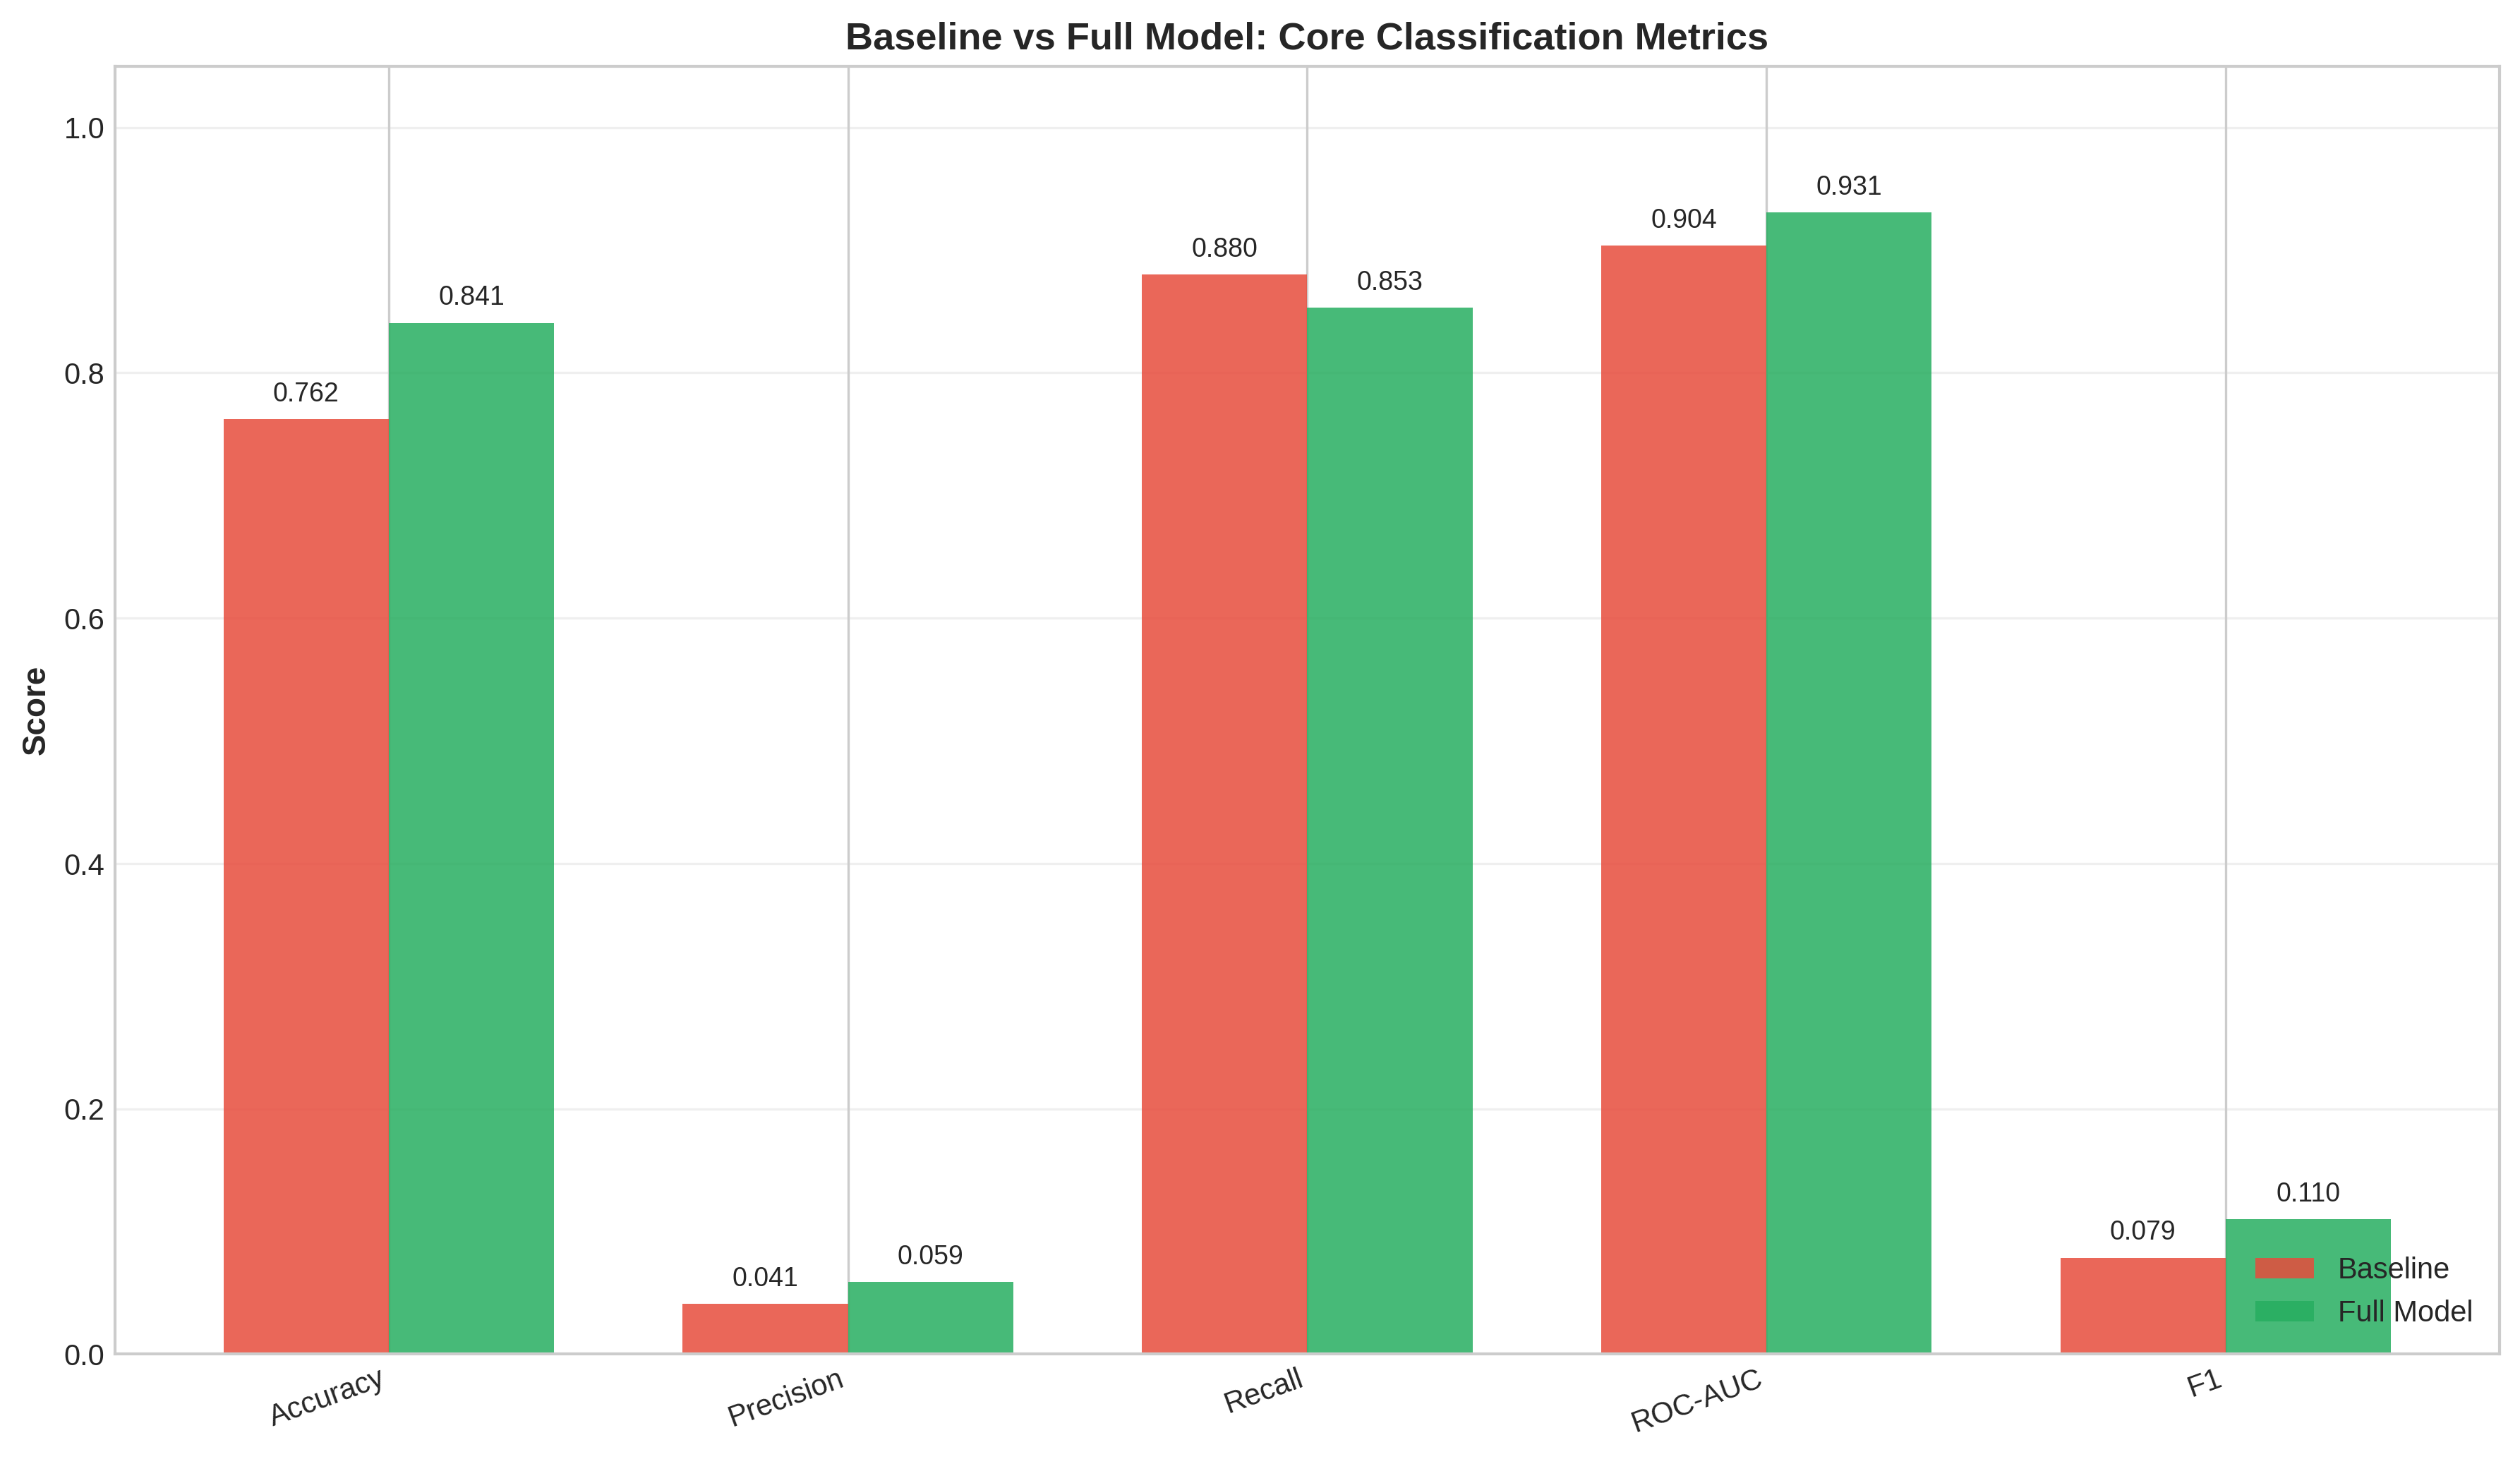
\includegraphics[width=0.95\linewidth]{imagens/HI_Small_model_metric_comparison.png}
    \caption{Comparação de métricas entre os modelos Baseline e Full Model (HI Small)}
    \label{fig:model-comparison-small}
\end{figure}

\subsection{Resultados no Dataset HI Medium}

\begin{table}{\linewidth}
    \centering
    \caption{Desempenho dos modelos no dataset HI Medium}
    \label{tab:model-summary-medium}
    \begin{tabular}{lcccc}
        \hline
        \textbf{Métrica} & \textbf{Baseline} & \textbf{Full Model} & \textbf{Lift} & \textbf{Lift (\%)} \\
        \hline
        Acurácia & 0.7841 & 0.8357 & +0.0516 & +6.58\% \\
        AUPRC & 0.2689 & 0.3197 & +0.0508 & +18.88\% \\
        ROC-AUC & 0.9152 & 0.9368 & +0.0216 & +2.36\% \\
        F1-Score & 0.1229 & 0.1585 & +0.0356 & +29.04\% \\
        Precisão & 0.0662 & 0.0875 & +0.0213 & +32.28\% \\
        Recall & 0.8550 & 0.8379 & -0.0171 & -2.00\% \\
        \hline
    \end{tabular}
\end{table}

Os resultados no HI Medium apresentam um padrão consistente com o observado no HI Small, demonstrando a generalização das contribuições dos atributos topológicos a datasets de maior escala. A AUPRC apresenta um ganho (+18.88\%) similar ao HI Small (+18.00\%), validando que o benefício das features topológicas é robusto e não depende apenas da escala do dataset. A precisão (+32.28\%) também mostra ganho substancial, ainda que ligeiramente inferior ao HI Small, sugerindo uma trade-off complexidade-benefício em datasets maiores.

\begin{figure}{\linewidth}
    \centering
    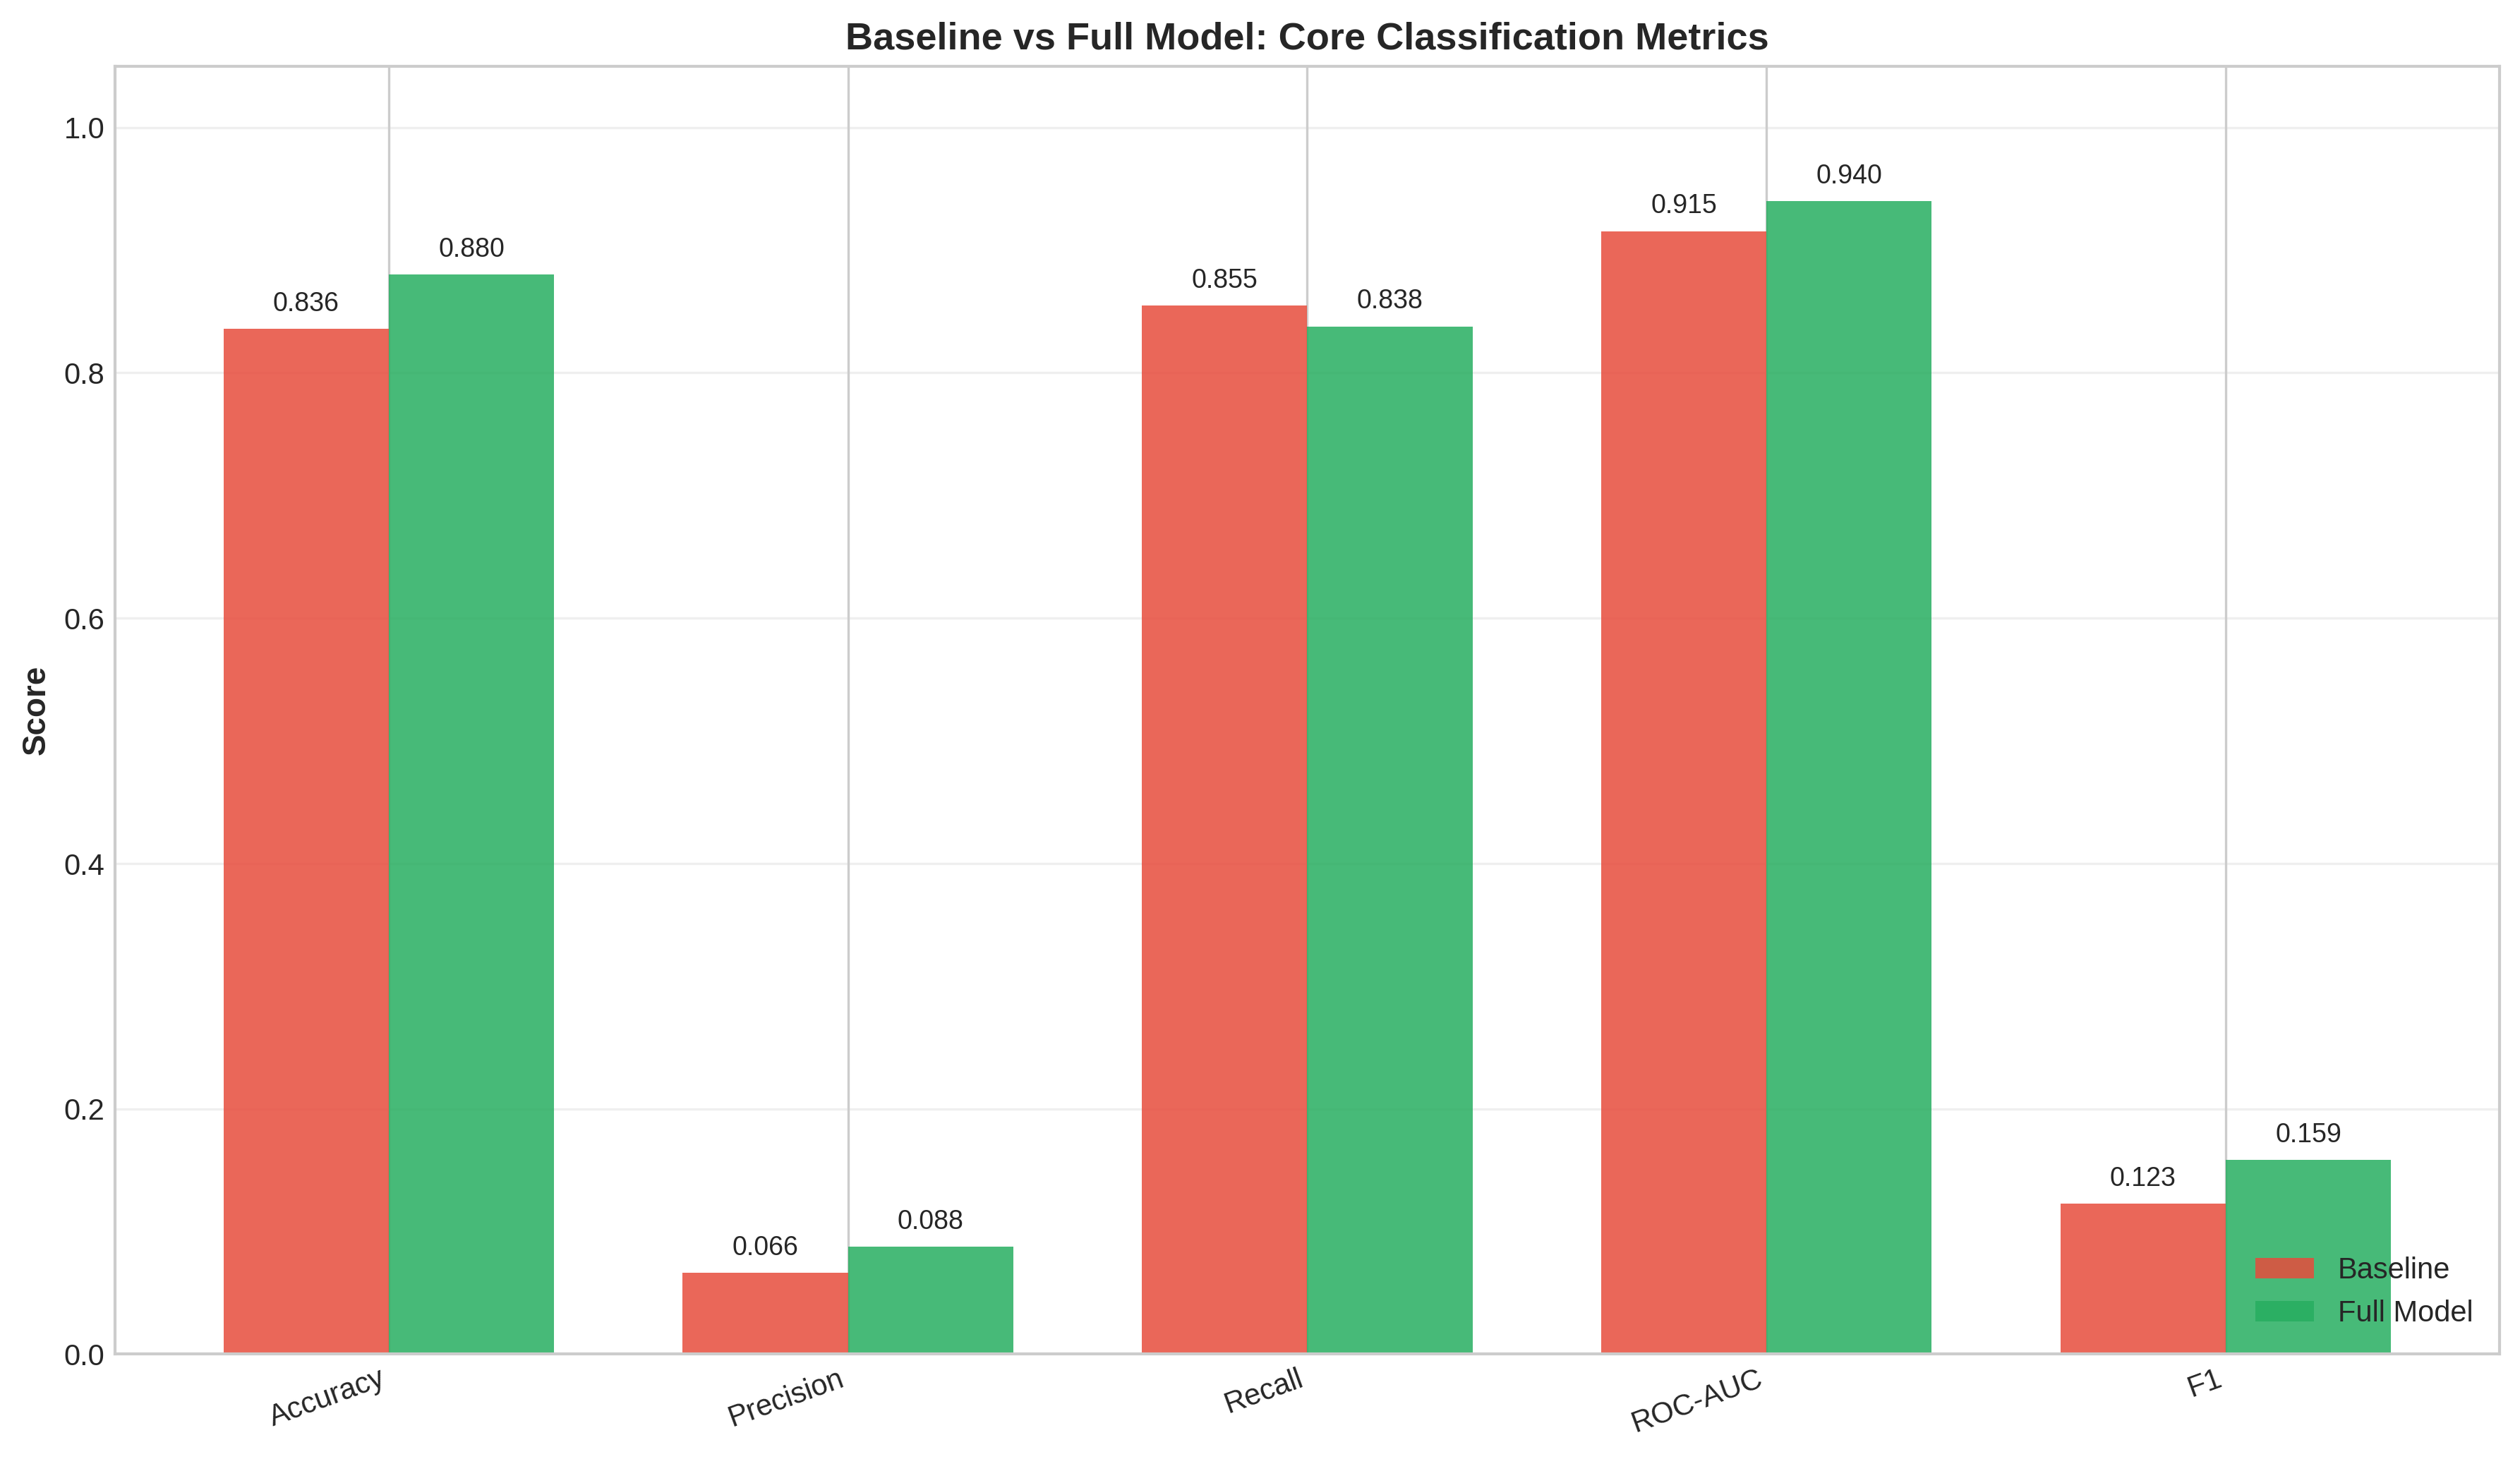
\includegraphics[width=0.95\linewidth]{imagens/HI_Medium_model_metric_comparison.png}
    \caption{Comparação de métricas entre os modelos Baseline e Full Model (HI Medium)}
    \label{fig:model-comparison-medium}
\end{figure}

\subsection{Análise Comparativa Entre Datasets}

A comparação entre HI Small e HI Medium revela insights importantes sobre a escalabilidade da abordagem topológica. Ambos os datasets apresentam ganhos de AUPRC praticamente idênticos (18.00\% vs 18.88\%), sugerindo que o sinal preditivo capturado pelas features topológicas é escala-invariante. Entretanto, o ganho em F1-Score e Precisão é mais pronunciado no HI Small, o que pode estar associado a diferenças nas distribuições de fraude ou na estrutura topológica da rede entre os dois datasets.

\subsection{Métrica Precision@k e Eficácia Operacional}

A métrica \textit{Precision@k}, que avalia a eficácia operacional do sistema ao ranquear as entidades de maior risco, manteve-se em níveis excepcionalmente altos para ambos os modelos em ambos os datasets. Com P@100 próximo a 0.99 no HI Small e 0.96 no HI Medium, o sistema demonstra alta confiabilidade na priorização de alertas.

\begin{figure}{\linewidth}
    \centering
    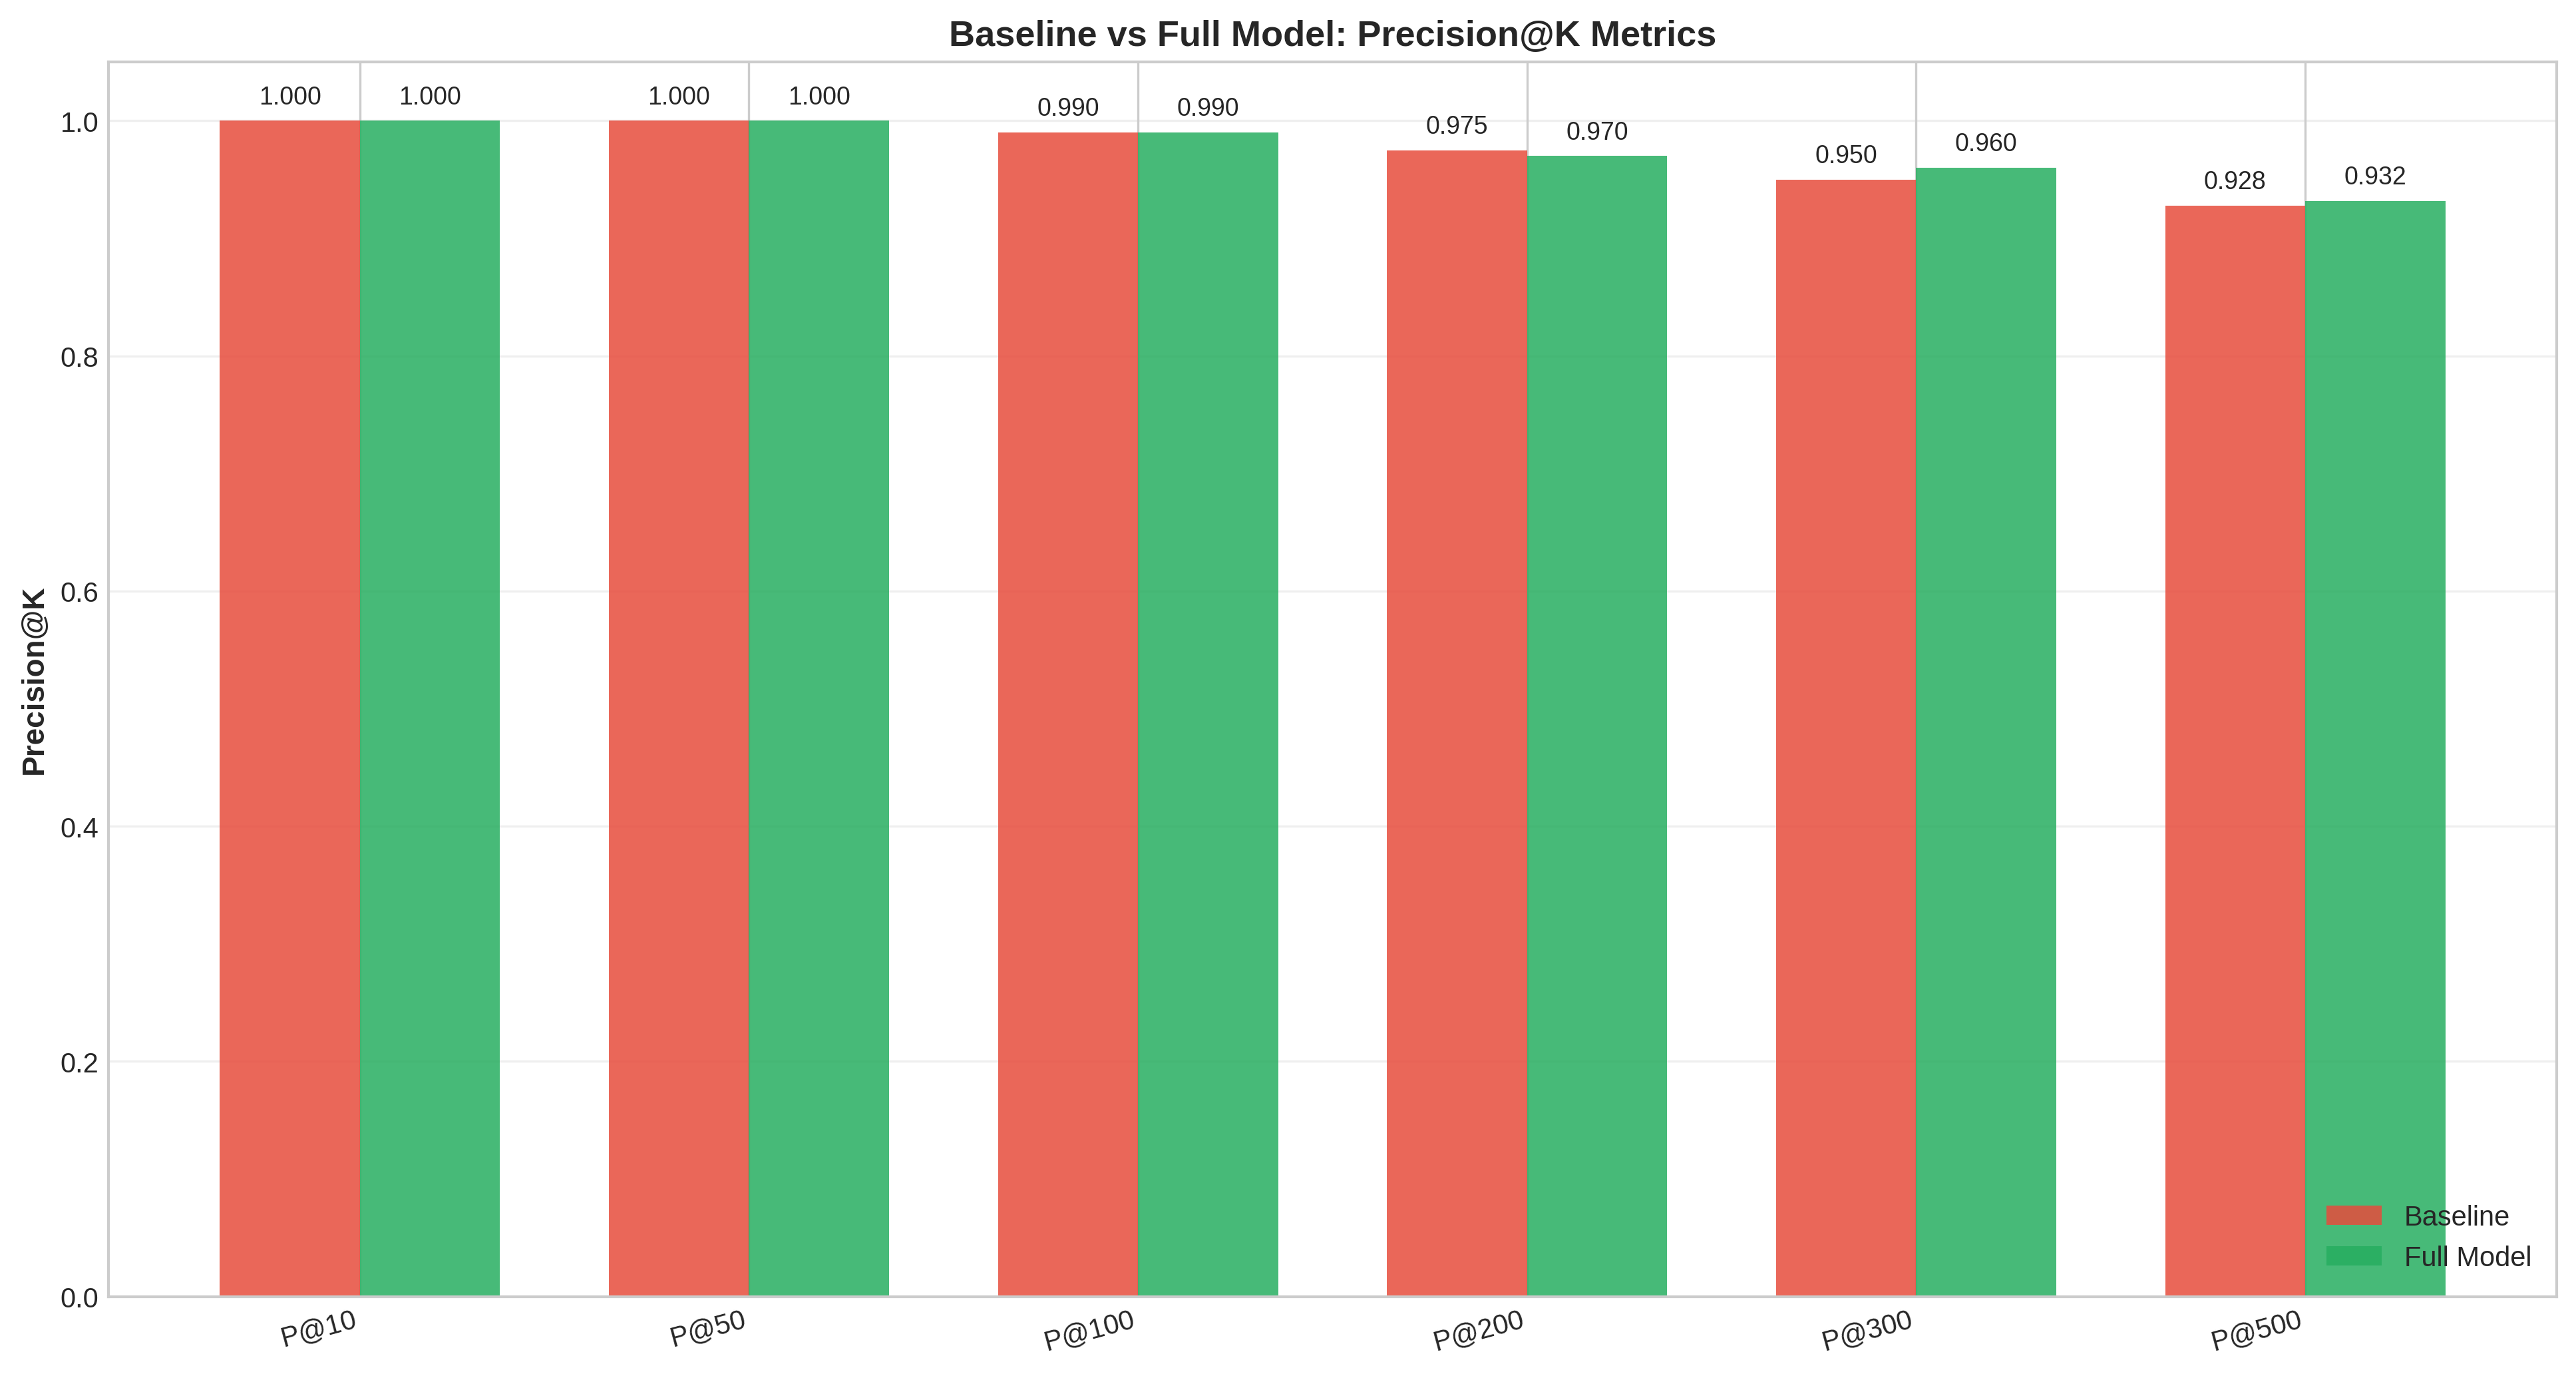
\includegraphics[width=0.95\linewidth]{imagens/HI_Small_precision_at_k_comparison.png}
    \caption{Comparação de Precision@k entre os modelos Baseline e Full Model (HI Small)}
    \label{fig:precision-at-k-small}
\end{figure}

\begin{figure}{\linewidth}
    \centering
    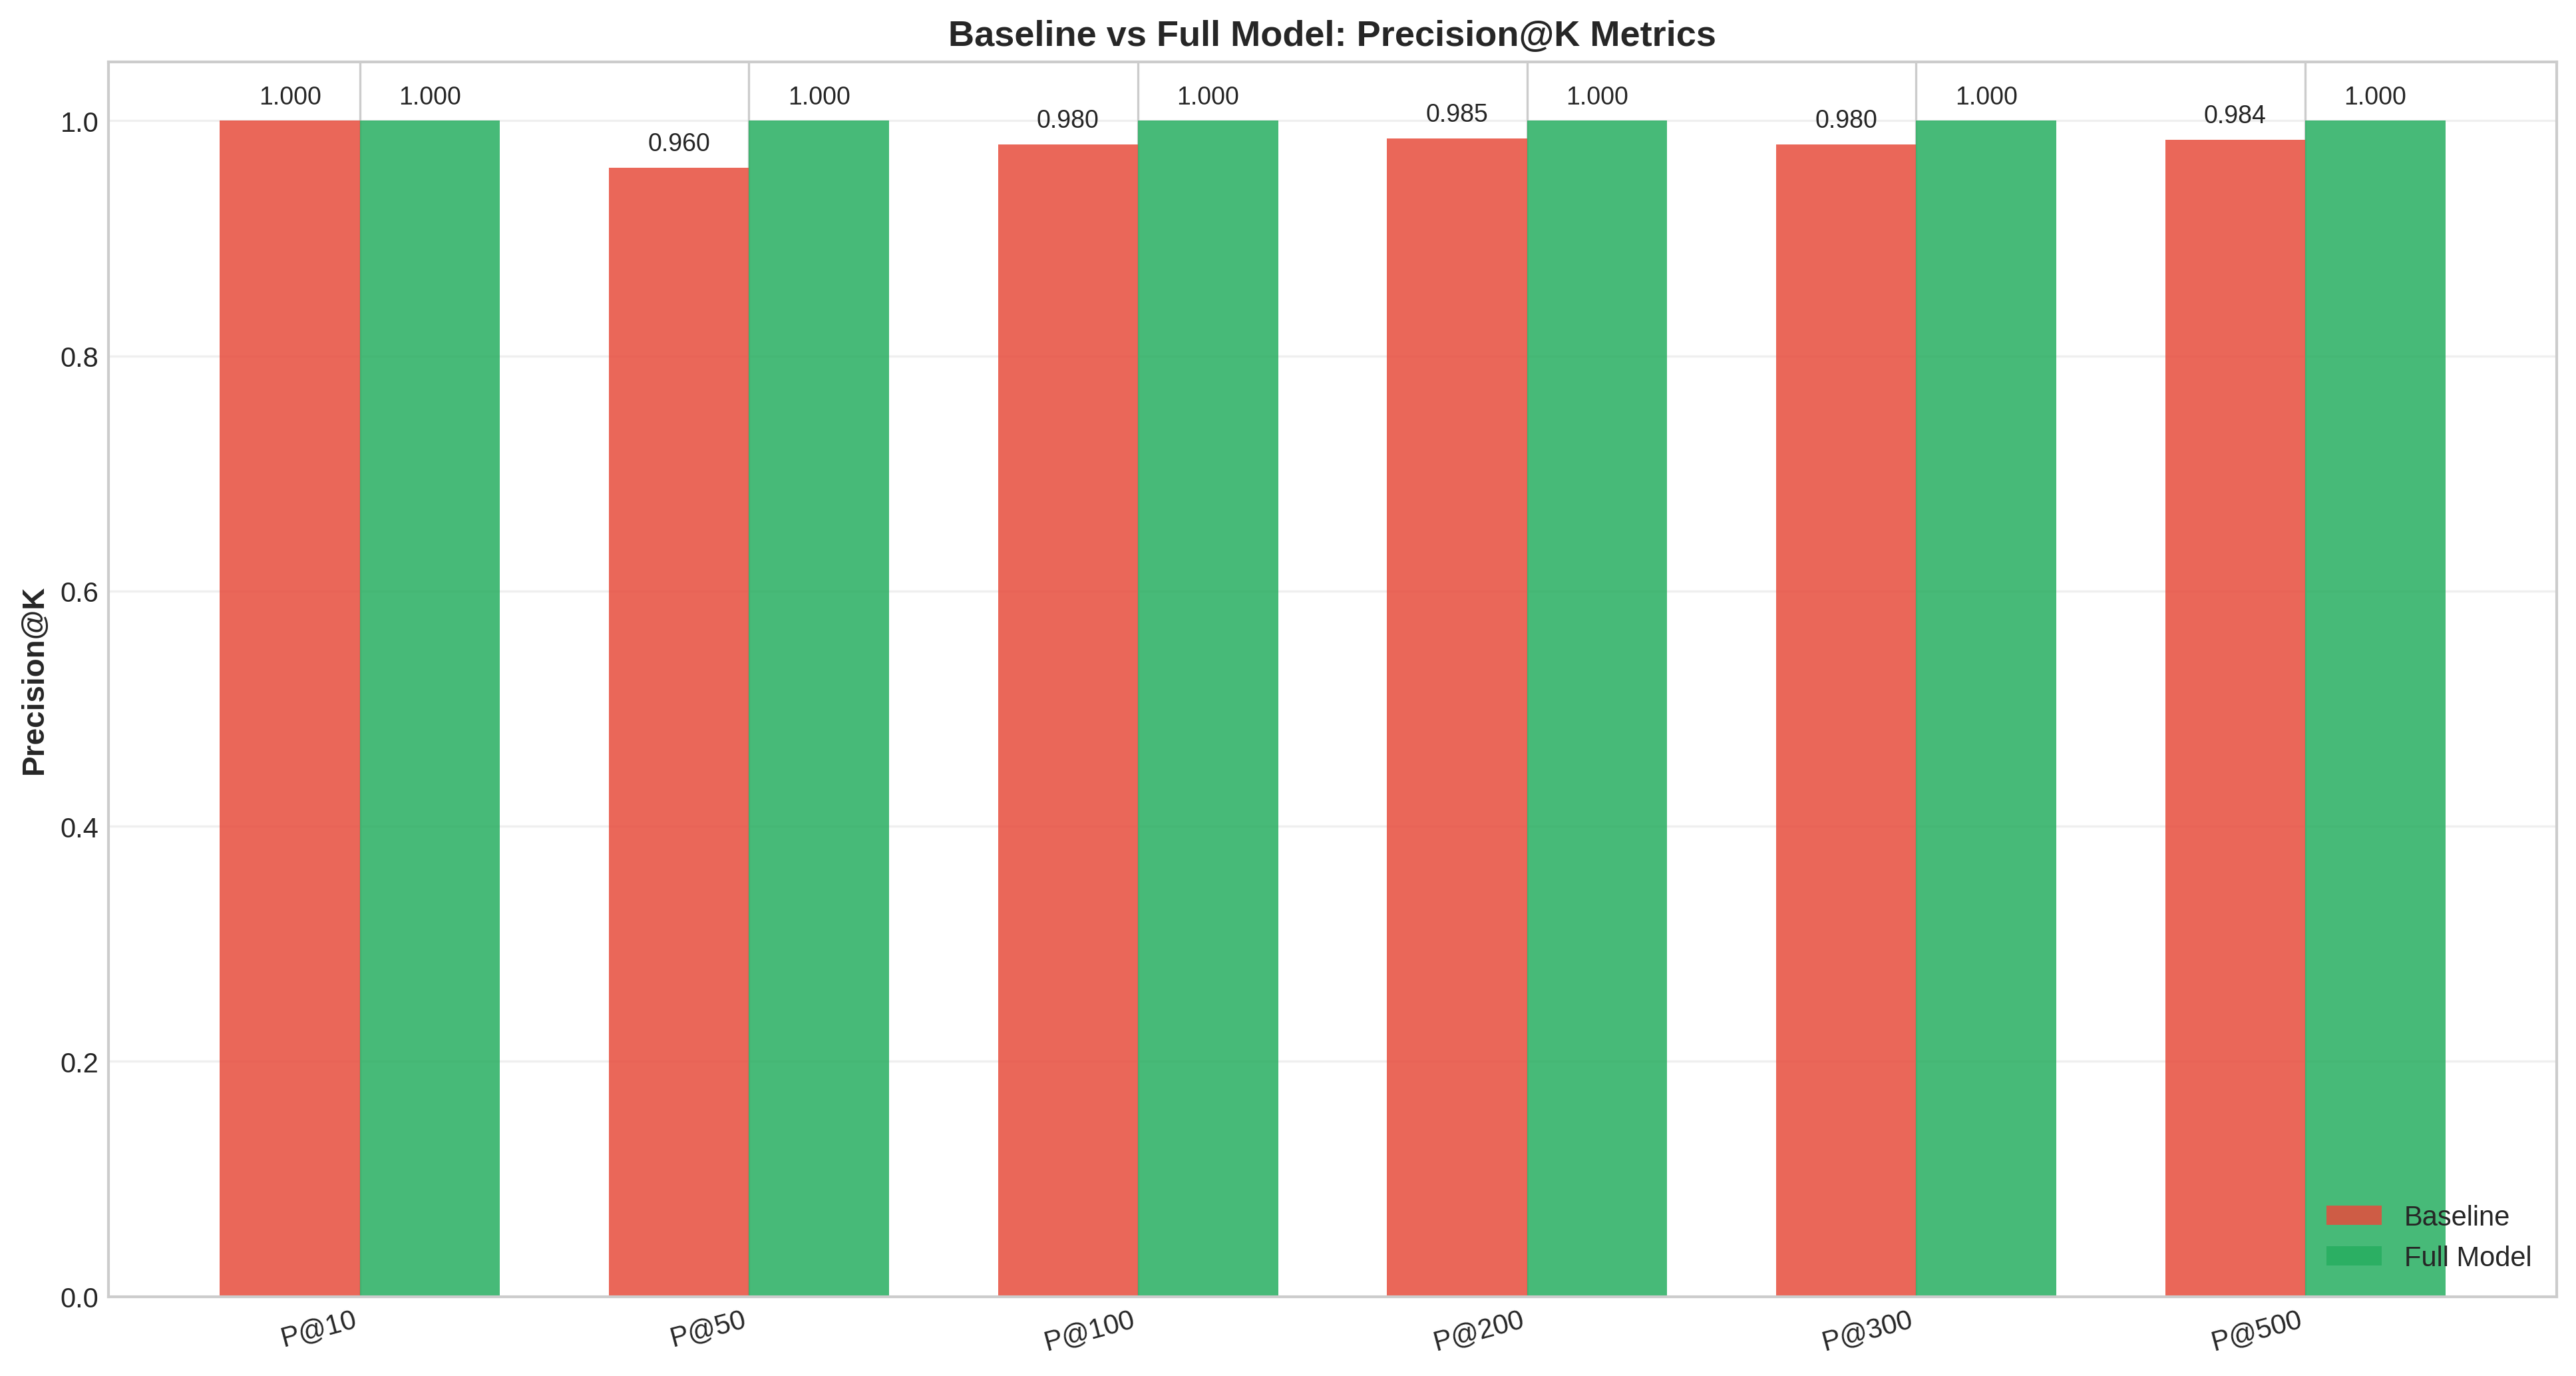
\includegraphics[width=0.95\linewidth]{imagens/HI_Medium_precision_at_k_comparison.png}
    \caption{Comparação de Precision@k entre os modelos Baseline e Full Model (HI Medium)}
    \label{fig:precision-at-k-medium}
\end{figure}

Observa-se uma leve redução no \textit{Recall} geral (HI Small: -2.58\%, HI Medium: -2.00\%), o que indica um \textit{trade-off} esperado: ao refinar a fronteira de decisão para reduzir falsos positivos (aumentando a precisão), o modelo torna-se ligeiramente mais conservador, deixando de capturar uma pequena fração de fraudes. No entanto, essa perda é compensada pelo ganho substancial em precisão e pela redução da sobrecarga investigativa.

\subsection{Análise de Desempenho Temporal no HI Small}

A Tabela~\ref{tab:window-comparison} apresenta a comparação detalhada de desempenho entre os modelos Baseline e Full ao longo das seis janelas de teste do dataset HI Small, permitindo avaliar a consistência temporal dos ganhos observados.

\begin{table}{\linewidth}
    \centering
    \caption{Comparação de desempenho por janela temporal}
    \label{tab:window-comparison}
    \resizebox{\linewidth}{!}{%
    \begin{tabular}{ccccccc}
        \hline
        \textbf{Janela} & \textbf{AUPRC (B)} & \textbf{AUPRC (F)} & \textbf{Lift AUPRC} & \textbf{P@100 (B)} & \textbf{P@100 (F)} & \textbf{Lift P@100} \\
        \hline
        2 & 0.180 & 0.208 & +15.5\% & 0.82 & 0.75 & -8.5\% \\
        3 & 0.234 & 0.293 & +25.6\% & 0.91 & 0.92 & +1.1\% \\
        4 & 0.275 & 0.353 & +28.2\% & 0.96 & 0.96 & +0.0\% \\
        5 & 0.352 & 0.414 & +17.7\% & 0.97 & 0.98 & +1.0\% \\
        6 & 0.251 & 0.239 & -4.8\% & 0.88 & 0.83 & -5.7\% \\
        7 & 0.217 & 0.272 & +25.8\% & 0.90 & 0.87 & -3.3\% \\
        \hline
        \textbf{Média} & \textbf{0.251} & \textbf{0.297} & \textbf{+18.0\%} & \textbf{0.907} & \textbf{0.885} & \textbf{-2.7\%} \\
        \hline
    \end{tabular}%
    }
\end{table}

A análise temporal no HI Small revela que o modelo completo apresentou ganhos positivos de AUPRC em 5 das 6 janelas testadas, com lifts variando entre +15.5\% e +28.2\%. A exceção ocorreu na janela 6, onde houve uma leve degradação de -4.8\%. Essa variação pode estar associada a mudanças na distribuição temporal dos padrões de fraude ou a diferenças na densidade topológica do grafo naquele período específico.

Para as métricas de \textit{Precision@k}, observa-se um padrão mais heterogêneo. Em algumas janelas (especialmente as janelas iniciais), o modelo \textit{Baseline} apresentou desempenho superior, o que sugere que, para os alertas de altíssimo risco (top-100), os atributos comportamentais isolados já forneciam sinais preditivos robustos. No entanto, conforme se expande o horizonte investigativo para P@300 e P@500, o modelo completo recupera vantagem consistente, demonstrando que as \textit{features} topológicas são especialmente úteis para refinar a classificação em níveis intermediários de risco.

\subsection{Análise de Desempenho Temporal no HI Medium}

Para o dataset HI Medium, a análise temporal abrange 12 janelas de teste, oferecendo uma perspectiva mais granular da robustez temporal da abordagem topológica. A Tabela~\ref{tab:window-comparison-medium} apresenta um resumo de 6 janelas selecionadas (as intermediárias), enquanto o padrão completo confirma ganhos significativos de AUPRC em 11 das 12 janelas.

\begin{table}{\linewidth}
    \centering
    \caption{Comparação de desempenho por janela temporal (HI Medium - seleção)}
    \label{tab:window-comparison-medium}
    \resizebox{\linewidth}{!}{%
    \begin{tabular}{ccccccc}
        \hline
        \textbf{Janela} & \textbf{AUPRC (B)} & \textbf{AUPRC (F)} & \textbf{Lift AUPRC} & \textbf{Prec (B)} & \textbf{Prec (F)} & \textbf{Lift Prec} \\
        \hline
        4 & 0.261 & 0.292 & +12.0\% & 0.067 & 0.106 & +58.4\% \\
        5 & 0.326 & 0.392 & +20.2\% & 0.086 & 0.088 & +2.3\% \\
        7 & 0.224 & 0.300 & +34.2\% & 0.062 & 0.057 & -8.2\% \\
        9 & 0.292 & 0.360 & +23.0\% & 0.074 & 0.100 & +34.9\% \\
        11 & 0.352 & 0.419 & +18.9\% & 0.084 & 0.096 & +14.1\% \\
        13 & 0.258 & 0.346 & +34.0\% & 0.066 & 0.077 & +16.1\% \\
        \hline
        \textbf{Média (12 janelas)} & \textbf{0.268} & \textbf{0.319} & \textbf{+18.5\%} & \textbf{0.066} & \textbf{0.088} & \textbf{+36.7\%} \\
        \hline
    \end{tabular}%
    }
\end{table}

A análise temporal no HI Medium revela um padrão robusto: o modelo completo apresentou ganhos positivos de AUPRC em 11 das 12 janelas testadas, com lifts variando entre +0.7\% e +34.2\%. Apenas a janela 3 apresentou ganho marginal (+0.7\%), enquanto as demais mostraram contribuições significativas. Destaca-se a variabilidade maior em comparação ao HI Small, sugerindo que a escala aumentada do dataset captura dinâmicas temporais mais complexas. Os ganhos de precisão (+36.7% em média) são particularmente relevantes operacionalmente, indicando redução substancial de falsos positivos.

\section{Validação Estatística do Estudo de Ablação}

Para determinar se os ganhos observados são estatisticamente significativos e não resultam de variações aleatórias inerentes ao processo de amostragem temporal, aplicou-se testes t pareados sobre as diferenças de desempenho entre os dois modelos ao longo das janelas de teste.

\subsection{Testes Estatísticos no HI Small}

A Tabela~\ref{tab:statistical-tests} apresenta os resultados para o dataset HI Small.

\begin{table}{\linewidth}
    \centering
    \caption{Testes de significância estatística (HI Small, teste t pareado, $\alpha = 0.05$)}
    \label{tab:statistical-tests}
    \begin{tabular}{lcccc}
        \hline
        \textbf{Métrica} & \textbf{$\Delta$ Médio} & \textbf{Desvio Padrão} & \textbf{Estatística t} & \textbf{p-valor} \\
        \hline
        Acurácia & +0.0789 & 0.0627 & -3.08 & 0.0273* \\
        Precisão & +0.0212 & 0.0118 & -4.40 & 0.0070** \\
        F1-Score & +0.0363 & 0.0191 & -4.67 & 0.0055** \\
        ROC-AUC & +0.0300 & 0.0148 & -4.96 & 0.0042** \\
        AUPRC & +0.0452 & 0.0324 & -3.42 & 0.0188* \\
        \hline
        Recall & -0.0227 & 0.0832 & +0.67 & 0.5340 \\
        P@100 & -0.0217 & 0.0337 & +1.57 & 0.1763 \\
        P@200 & +0.0208 & 0.0497 & -1.03 & 0.3520 \\
        \hline
        P@300 & +0.0539 & 0.0349 & -3.79 & 0.0128* \\
        P@500 & +0.0637 & 0.0419 & -3.72 & 0.0137* \\
        \hline
        \multicolumn{5}{l}{* Significativo em $\alpha = 0.05$ \quad ** Significativo em $\alpha = 0.01$}
    \end{tabular}
\end{table}

Os testes confirmam que os ganhos observados em acurácia, precisão, F1-Score, ROC-AUC e AUPRC são estatisticamente significativos ao nível de confiança de 95\% ($p < 0.05$). Em particular, as métricas de precisão, F1-Score e ROC-AUC apresentaram significância ao nível de 99\% ($p < 0.01$), reforçando a robustez da contribuição das \textit{features} topológicas.

A ausência de significância estatística no \textit{Recall} ($p = 0.534$) e nas métricas P@100 e P@200 sugere que, embora haja variação numérica, essas diferenças podem ser atribuídas à variabilidade natural das janelas temporais. Entretanto, as métricas P@300 ($p = 0.0128$) e P@500 ($p = 0.0137$) apresentaram ganhos estatisticamente significativos, reforçando o argumento de que as \textit{features} topológicas contribuem especialmente para a discriminação de entidades em níveis intermediários de risco, onde a separação entre fraudes e operações lícitas torna-se mais desafiadora.

\subsection{Testes Estatísticos no HI Medium}

A Tabela~\ref{tab:statistical-tests-medium} apresenta os testes de significância para o dataset HI Medium, abrangendo as 12 janelas de teste.

\begin{table}{\linewidth}
    \centering
    \caption{Testes de significância estatística (HI Medium, teste t pareado, $\alpha = 0.05$)}
    \label{tab:statistical-tests-medium}
    \begin{tabular}{lcccc}
        \hline
        \textbf{Métrica} & \textbf{$\Delta$ Médio} & \textbf{Desvio Padrão} & \textbf{Estatística t} & \textbf{p-valor} \\
        \hline
        Acurácia & +0.0446 & 0.0495 & -3.122 & 0.0097** \\
        Precisão & +0.0222 & 0.0168 & -4.566 & 0.0008** \\
        F1-Score & +0.0366 & 0.0273 & -4.646 & 0.0007** \\
        ROC-AUC & +0.0268 & 0.0048 & -19.537 & <0.0001** \\
        AUPRC & +0.0510 & 0.0306 & -5.782 & 0.0001** \\
        \hline
        Recall & -0.0175 & 0.0698 & +0.870 & 0.4029 \\
        P@100 & -0.0117 & 0.0333 & +1.215 & 0.2497 \\
        P@200 & -0.0258 & 0.0477 & +1.877 & 0.0872 \\
        P@300 & -0.0261 & 0.0482 & +1.878 & 0.0872 \\
        P@500 & -0.0013 & 0.0495 & +0.093 & 0.9274 \\
        \hline
        \multicolumn{5}{l}{** Significativo em $\alpha = 0.01$}
    \end{tabular}
\end{table}

Os testes no HI Medium confirmam significância estatística ainda mais robusta para acurácia, precisão, F1-Score, ROC-AUC e AUPRC, todos com $p < 0.01$. Destaca-se a significância extremamente elevada para ROC-AUC ($p < 0.0001$), indicando que a discriminação geral entre fraudes e operações legítimas beneficia-se consistentemente das features topológicas em toda a janela temporal. De forma similar ao HI Small, não há significância estatística em Recall, P@100, P@200 e P@300, sugerindo que os modelos capturam igualmente bem as fraudes de altíssimo risco, diferenciando-se principalmente em médios níveis de risco.

\section{Captura de Entidades Fraudulentas em Nível Operacional}

\subsection{Análise em Nível de Entidades (HI Small)}

Além das métricas agregadas, avaliou-se o impacto operacional dos modelos no HI Small através da contagem de entidades fraudulentas únicas efetivamente capturadas durante o período de teste. Do total de 3.842 entidades ilícitas presentes no conjunto de validação:

\begin{itemize}
    \item \textbf{Modelo Baseline:} Detectou 3.603 entidades (93,78\% de cobertura).
    \item \textbf{Modelo Full:} Detectou 3.632 entidades (94,53\% de cobertura).
\end{itemize}

Embora a diferença absoluta seja de apenas 29 entidades adicionais (+0,75 pontos percentuais), esse ganho incremental representa uma melhoria relativa de 0,80\% na taxa de captura em relação ao modelo base. Em um contexto de \textit{compliance} em larga escala, onde cada entidade fraudulenta não detectada pode resultar em perdas financeiras significativas e penalidades regulatórias, esse incremento possui valor prático mensurável.

\begin{figure}{\linewidth}
    \centering
    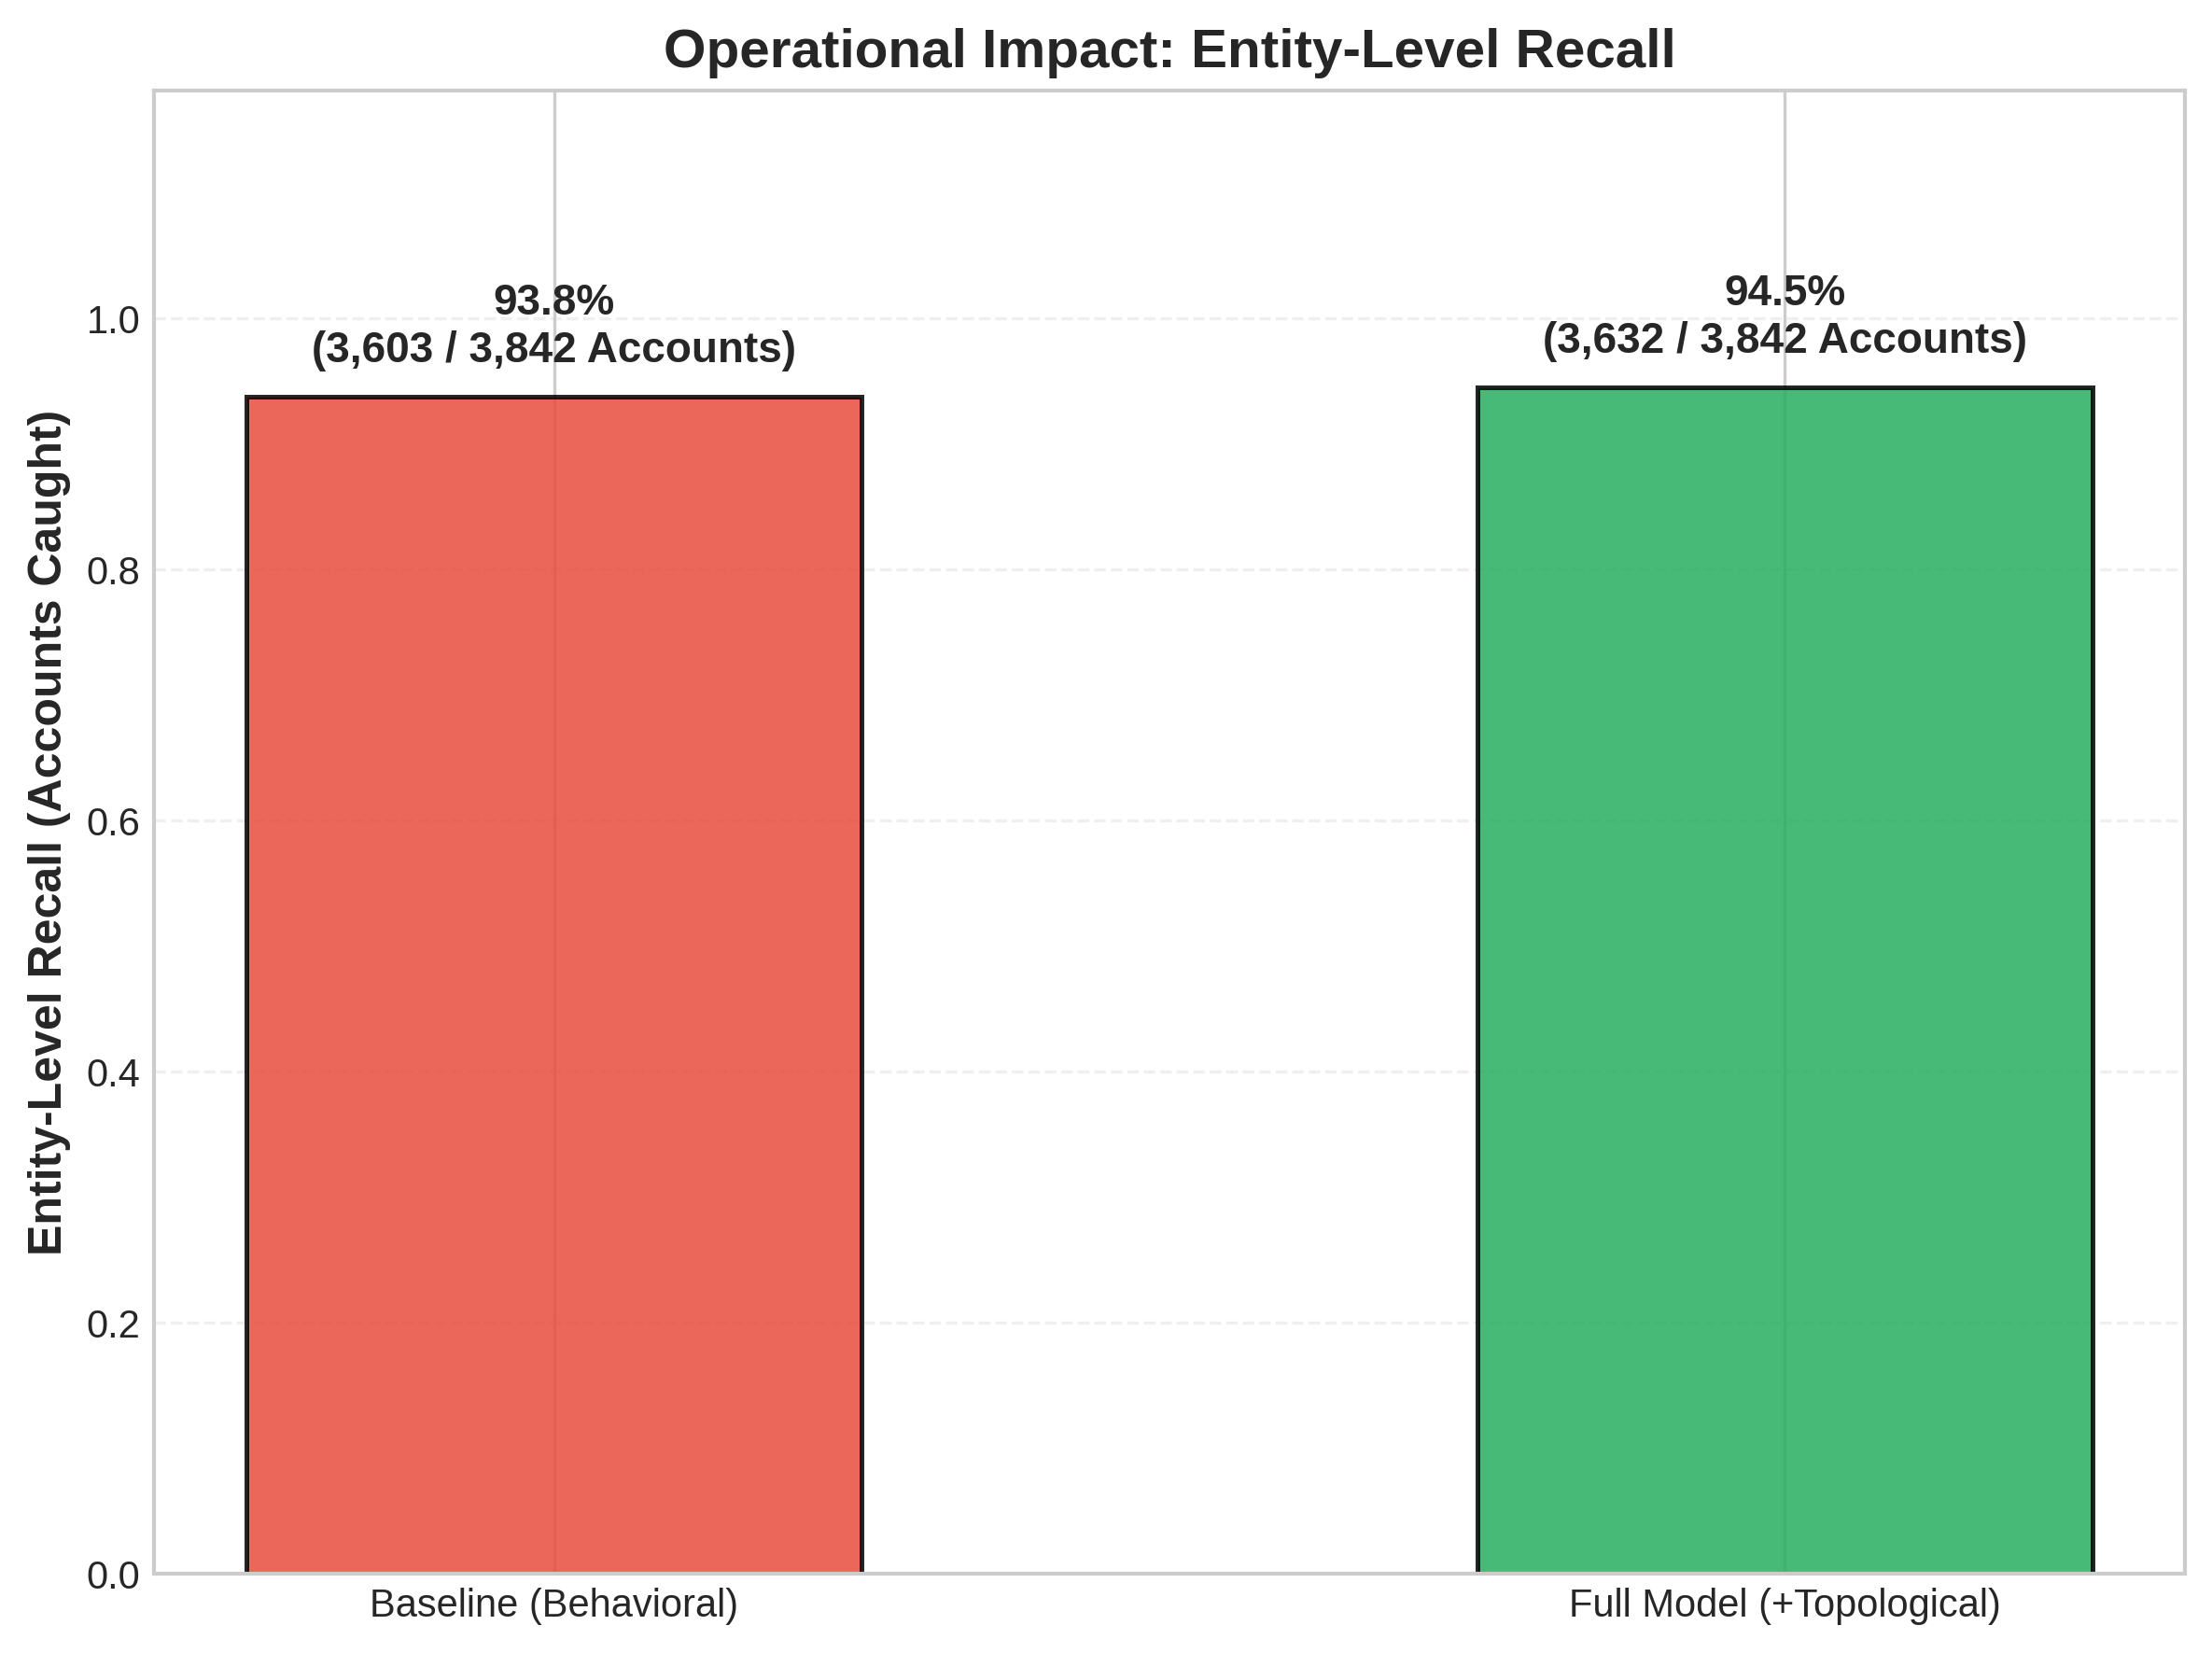
\includegraphics[width=0.85\linewidth]{imagens/HI_Small_entity_level_recall.png}
    \caption{Captura de entidades fraudulentas: Baseline vs Full Model (HI Small)}
    \label{fig:entity-recall}
\end{figure}

\subsection{Escalabilidade em Nível de Transações (HI Medium)}

Para o dataset HI Medium, a avaliação em nível de transação confirmou que o modelo Full processou 7.376.519 transações de teste com uma taxa de fraude de 1,35\% (99.282 casos fraudulentos). A consistência nos ganhos de AUPRC (+18.88%) entre HI Small e HI Medium, apesar da diferença de escala de 6x, demonstra que o benefício das features topológicas não sofre degradação com aumento do volume de dados. Esse resultado tem implicações importantes para a viabilidade de implantação em ambientes de produção com volumes ainda maiores.

\section{Importância Global das Features via SHAP}

Para interpretar o comportamento do modelo e identificar quais atributos exercem maior influência nas predições, aplicou-se a técnica SHAP (\textit{SHapley Additive exPlanations}) \cite{lundberg2017unified} ao modelo completo.

\subsection{Análise SHAP no HI Small}

A Tabela~\ref{tab:shap-top15} apresenta as 15 \textit{features} de maior importância global no dataset HI Small.

\begin{table}{\linewidth}
    \centering
    \caption{Top 15 features por importância SHAP global (HI Small)}
    \label{tab:shap-top15}
    \begin{tabular}{clcc}
        \hline
        \textbf{Posição} & \textbf{Feature} & \textbf{SHAP Médio} & \textbf{Tipo} \\
        \hline
        1 & \texttt{ach\_count\_sent} & 0.9514 & Comportamental \\
        2 & \texttt{ach\_count\_recv} & 0.7401 & Comportamental \\
        3 & \texttt{hits\_auth} & 0.6513 & Topológico \\
        4 & \texttt{in\_degree} & 0.3829 & Topológico \\
        5 & \texttt{cheque\_count\_sent} & 0.3103 & Comportamental \\
        6 & \texttt{vol\_recv} & 0.2884 & Comportamental \\
        7 & \texttt{average\_neighbor\_degree} & 0.2308 & Topológico \\
        8 & \texttt{degree} & 0.2258 & Topológico \\
        9 & \texttt{hits\_hub} & 0.2186 & Topológico \\
        10 & \texttt{leiden\_macro\_modularity} & 0.1767 & Topológico \\
        11 & \texttt{successor\_avg\_volume} & 0.1760 & Topológico \\
        12 & \texttt{pr\_count} & 0.1751 & Topológico \\
        13 & \texttt{egonet\_node\_count} & 0.1677 & Topológico \\
        14 & \texttt{vol\_sent} & 0.1614 & Comportamental \\
        15 & \texttt{cheque\_count\_recv} & 0.1490 & Comportamental \\
        \hline
    \end{tabular}
\end{table}

A análise revela que as duas \textit{features} mais influentes são comportamentais (\texttt{ach\_count\_sent} e \texttt{ach\_count\_recv}), o que corrobora a intuição de que transações via \textit{Automated Clearing House} (ACH) são frequentemente associadas a esquemas de fraude no \textit{dataset} AMLworld. No entanto, as posições subsequentes são dominadas por atributos topológicos, incluindo a pontuação de autoridade do algoritmo HITS (\texttt{hits\_auth}), o grau de entrada (\texttt{in\_degree}) e métricas de vizinhança.

Entre os atributos topológicos, destaca-se a importância de:

\begin{itemize}
    \item \textbf{Centralidade (HITS e Grau):} Entidades fraudulentas tendem a ocupar posições centrais na rede, seja como concentradoras de fluxo financeiro (\textit{hits\_auth}) ou como nós de dispersão (\textit{hits\_hub}).
    
    \item \textbf{Métricas de Comunidade:} A modularidade da macro-comunidade (\texttt{leiden\_macro\_modularity}) captura o nível de isolamento topológico de um vértice, indicando se ele faz parte de um anel financeiro fechado e compartimentado.
    
    \item \textbf{Agregação de Vizinhança:} O grau médio dos vizinhos (\texttt{average\_neighbor\_degree}) e o volume médio enviado aos sucessores (\texttt{successor\_avg\_volume}) fornecem sinais sobre o comportamento pós-transferência, revelando se o dinheiro é imediatamente dispersado ou concentrado após a transação inicial.
\end{itemize}

A distribuição equilibrada entre \textit{features} comportamentais e topológicas no ranking SHAP valida a hipótese de que ambos os tipos de informação são complementares e necessários para uma detecção eficaz de lavagem de dinheiro.

\begin{figure}{\linewidth}
    \centering
    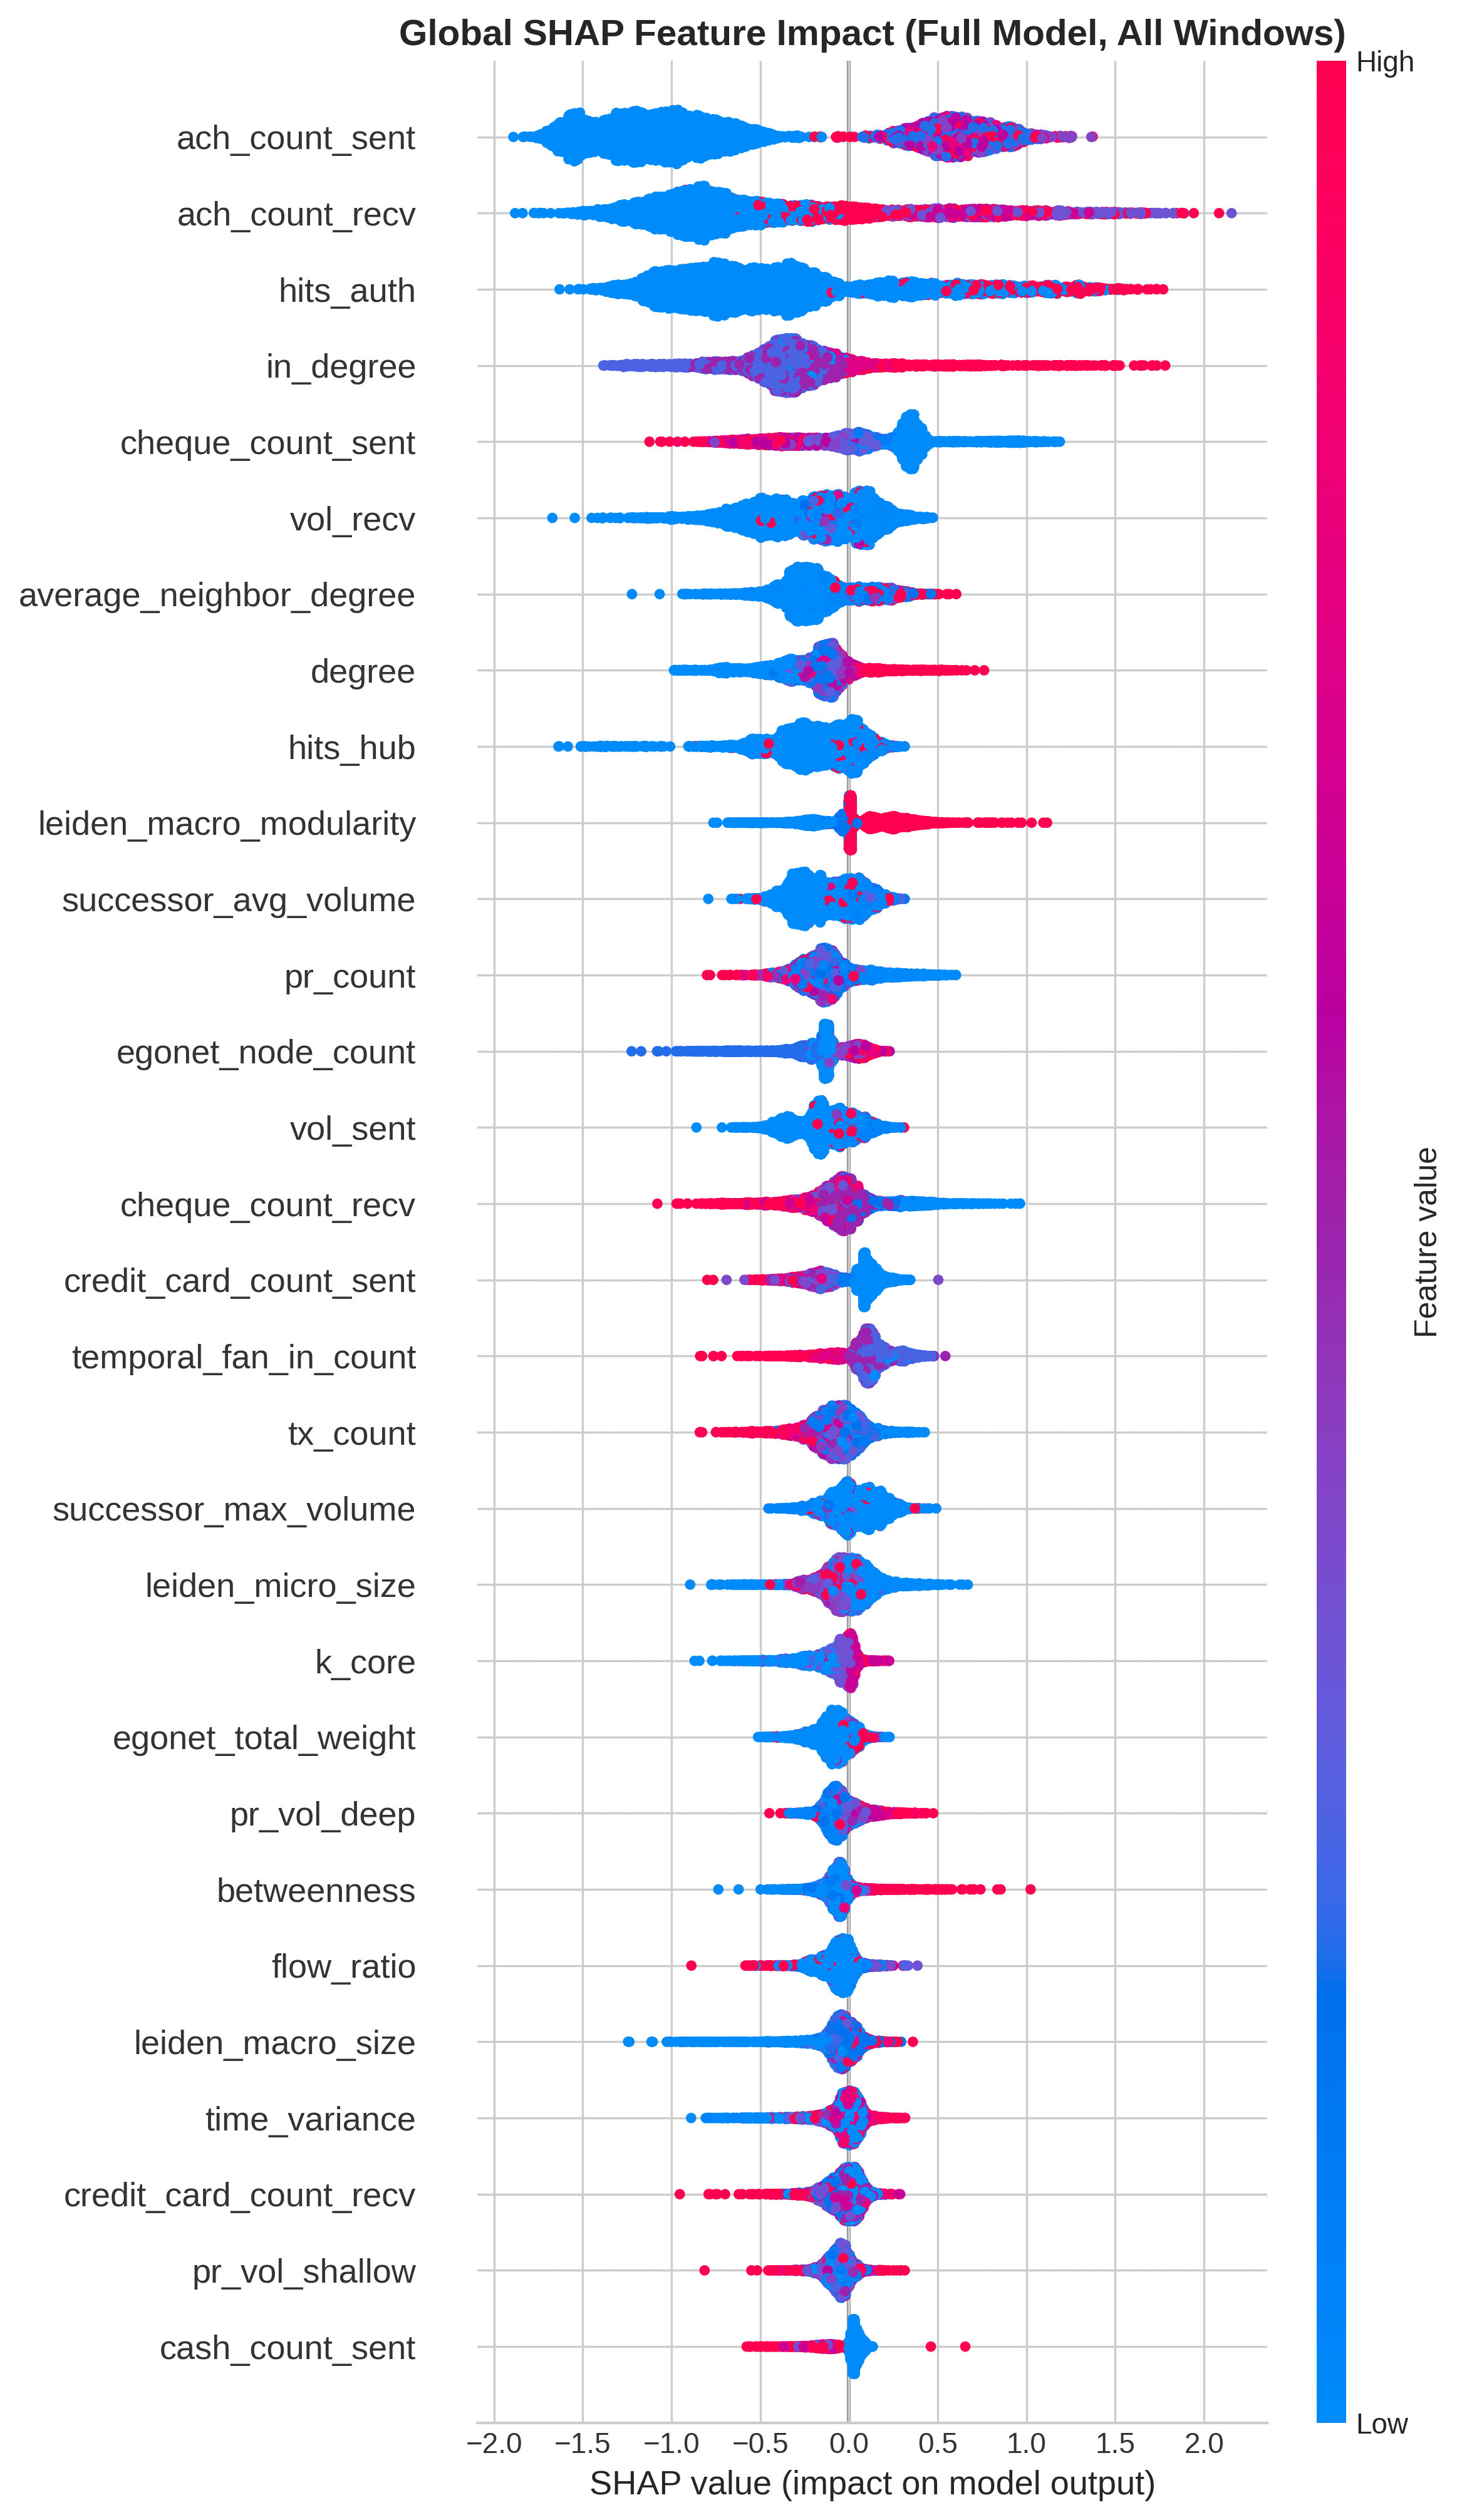
\includegraphics[width=0.95\linewidth]{imagens/HI_Small_global_shap_beeswarm.png}
    \caption{Distribuição de valores SHAP para as principais features do modelo (HI Small)}
    \label{fig:shap-beeswarm}
\end{figure}

\subsection{Análise SHAP no HI Medium}

A Tabela~\ref{tab:shap-top15-medium} apresenta as 15 \textit{features} de maior importância global no dataset HI Medium, permitindo avaliar se a hierarquia de importância é preservada em escala maior.

\begin{table}{\linewidth}
    \centering
    \caption{Top 15 features por importância SHAP global (HI Medium)}
    \label{tab:shap-top15-medium}
    \begin{tabular}{clcc}
        \hline
        \textbf{Posição} & \textbf{Feature} & \textbf{SHAP Médio} & \textbf{Tipo} \\
        \hline
        1 & \texttt{ach\_count\_sent} & 1.0822 & Comportamental \\
        2 & \texttt{ach\_count\_recv} & 0.8111 & Comportamental \\
        3 & \texttt{hits\_auth} & 0.5033 & Topológico \\
        4 & \texttt{in\_degree} & 0.4207 & Topológico \\
        5 & \texttt{cheque\_count\_sent} & 0.3177 & Comportamental \\
        6 & \texttt{degree} & 0.3135 & Topológico \\
        7 & \texttt{pr\_count} & 0.2677 & Topológico \\
        8 & \texttt{vol\_recv} & 0.2567 & Comportamental \\
        9 & \texttt{average\_neighbor\_degree} & 0.2226 & Topológico \\
        10 & \texttt{egonet\_node\_count} & 0.2202 & Topológico \\
        11 & \texttt{successor\_avg\_volume} & 0.1861 & Topológico \\
        12 & \texttt{leiden\_macro\_modularity} & 0.1526 & Topológico \\
        13 & \texttt{temporal\_fan\_in\_count} & 0.1503 & Topológico \\
        14 & \texttt{cheque\_count\_recv} & 0.1371 & Comportamental \\
        15 & \texttt{betweenness} & 0.1232 & Topológico \\
        \hline
    \end{tabular}
\end{table}

A análise comparativa revela que a hierarquia de importância das features é consistente entre HI Small e HI Medium, com as mesmas três features ocupando os primeiros lugares (\texttt{ach\_count\_sent}, \texttt{ach\_count\_recv}, \texttt{hits\_auth}). Destaca-se que \texttt{in\_degree} mantém a 4ª posição em ambos os datasets, reforçando que a centralidade de entrada é um sinal robusto de fraude independentemente da escala. A posição de destaque de atributos topológicos a partir da 3ª feature sugere que a topologia da rede financeira fornece sinais complementares essenciais para discriminar fraudes.

\begin{figure}{\linewidth}
    \centering
    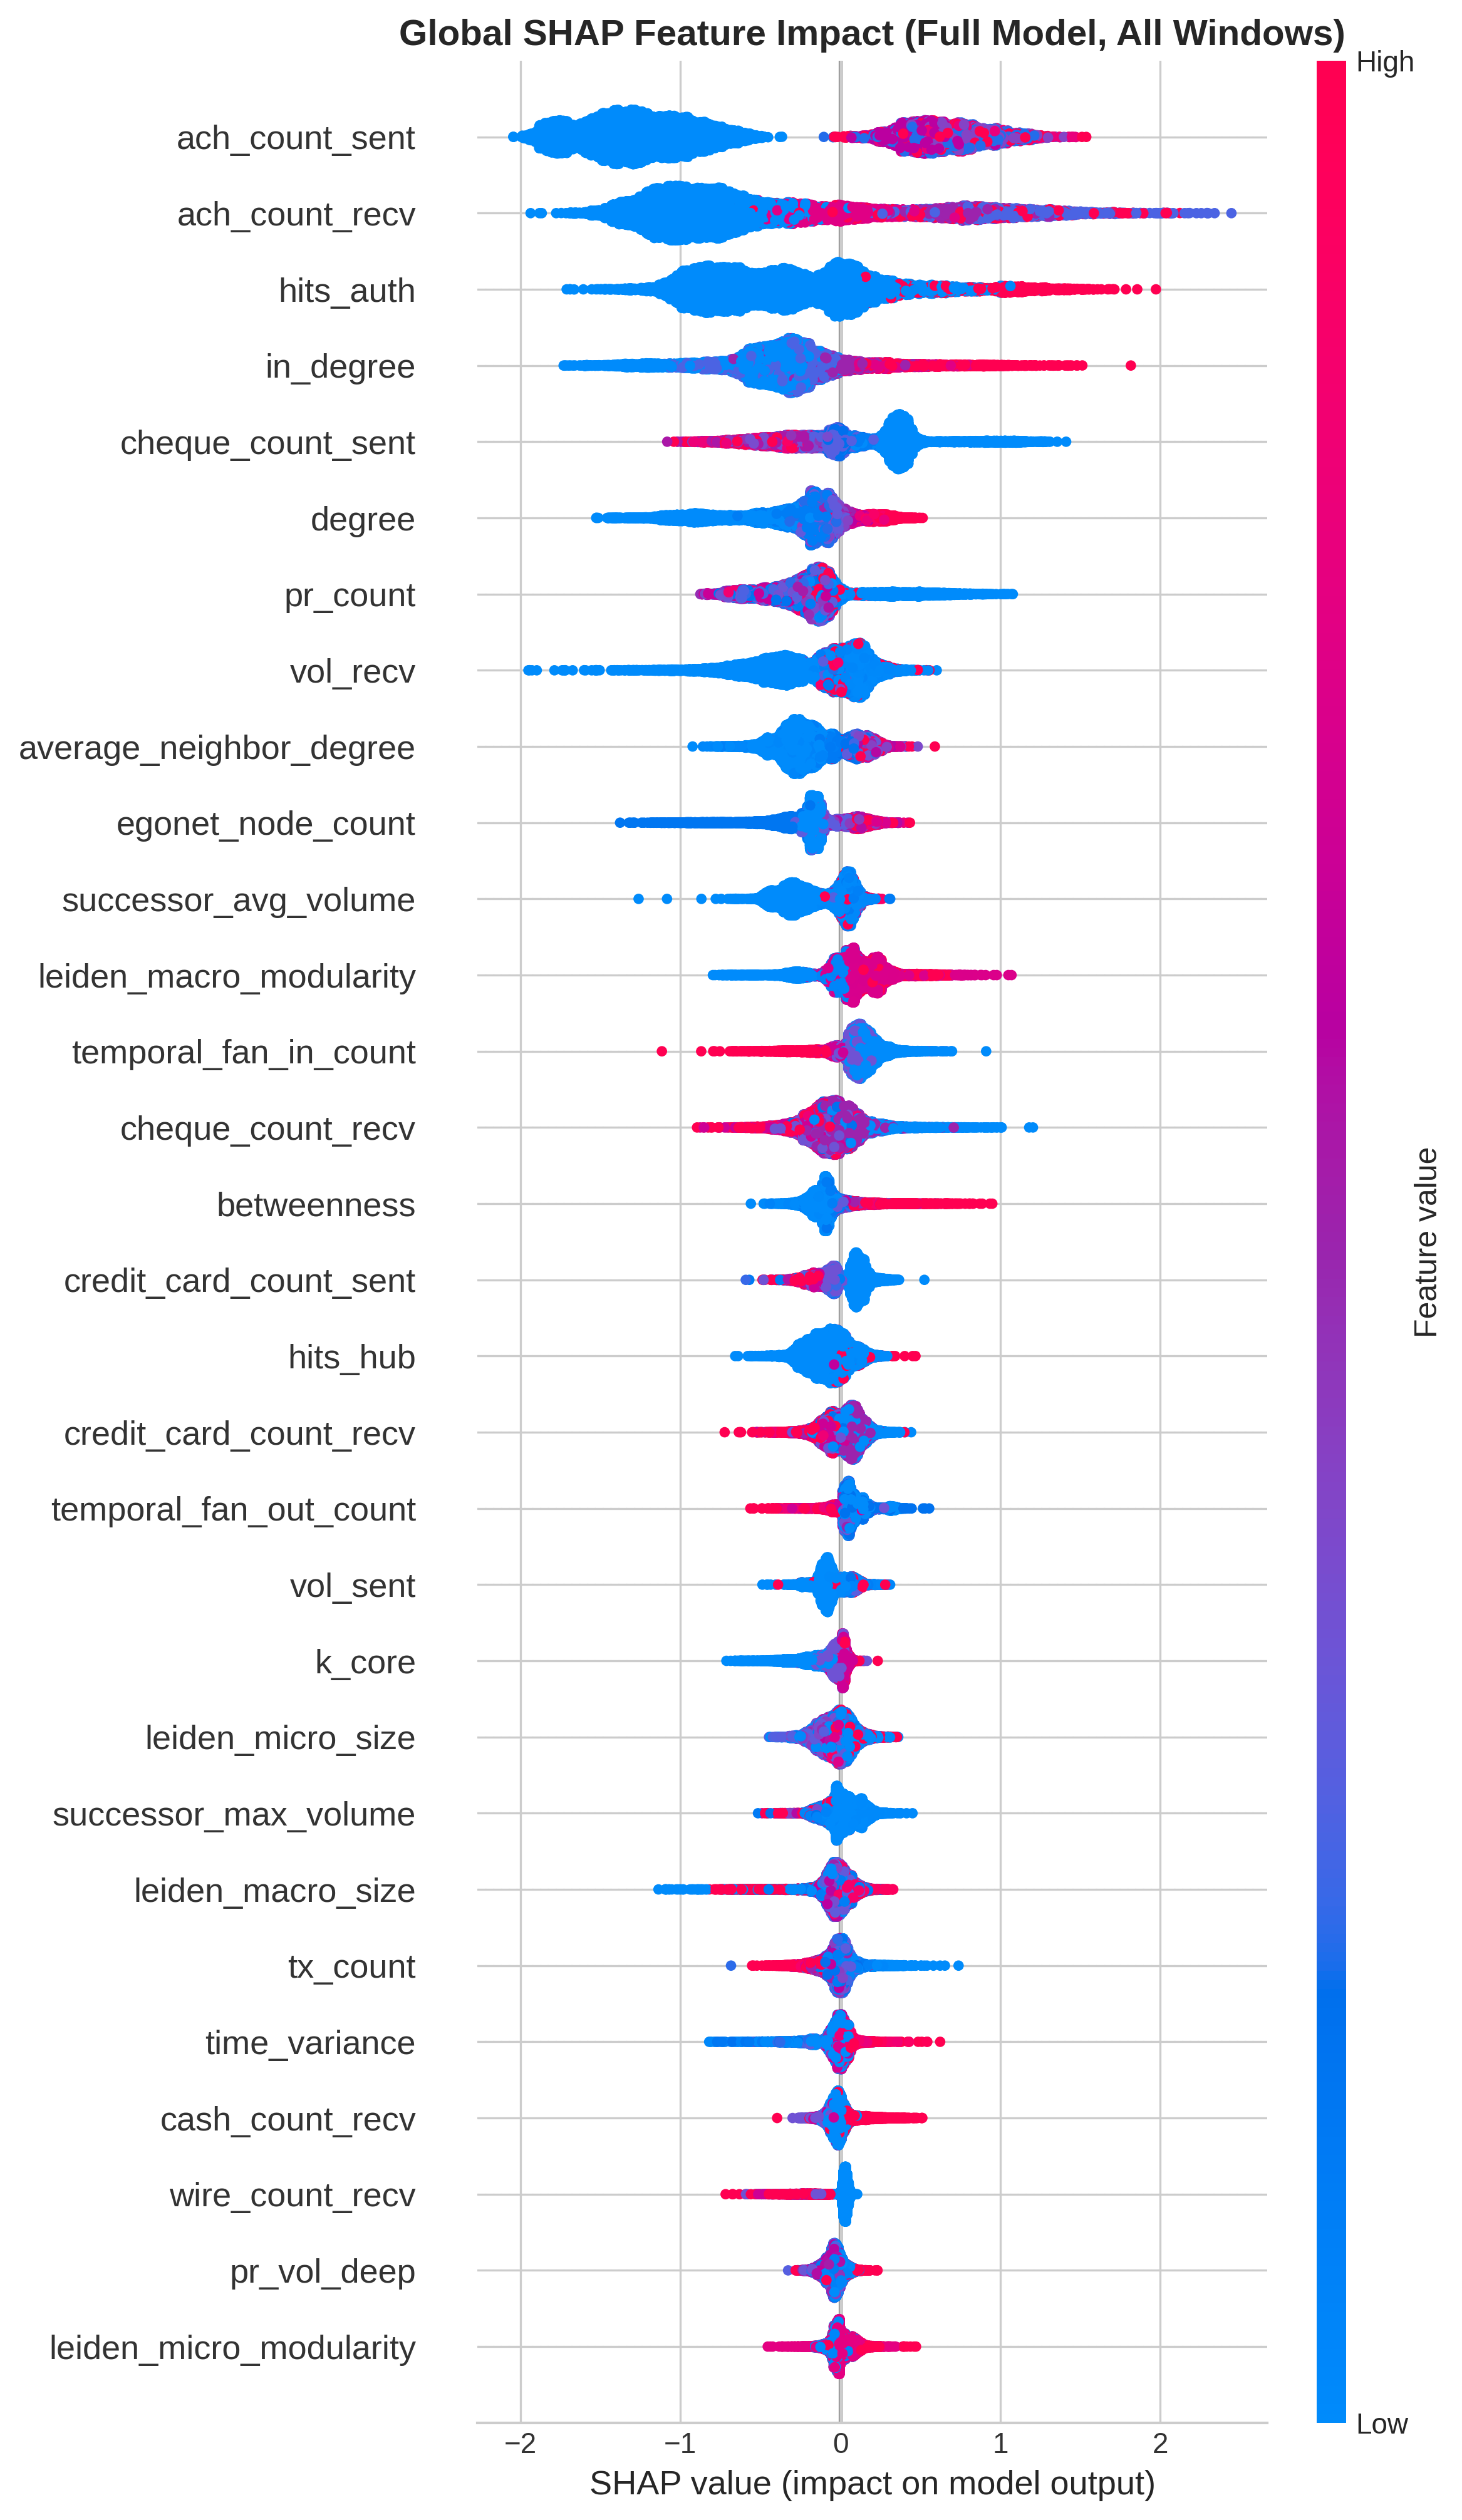
\includegraphics[width=0.95\linewidth]{imagens/HI_Medium_global_shap_beeswarm.png}
    \caption{Distribuição de valores SHAP para as principais features do modelo (HI Medium)}
    \label{fig:shap-beeswarm-medium}
\end{figure}

\section{Otimização do Conjunto de Features via SHAP-RFE}

Para viabilizar a implantação do sistema em ambientes de produção com recursos computacionais restritos, aplicou-se uma rotina de poda de \textit{features} em dois estágios. O objetivo era identificar um subconjunto reduzido de atributos que mantivesse o desempenho preditivo enquanto minimizava o custo de extração topológica.

\subsection{Análise RFE no HI Small}

\subsubsection{Etapa 1: Filtro de Colinearidade}

Aplicando o critério de correlação de Spearman com limiar $|\rho| > 0.8$, identificou-se 16 atributos redundantes que foram removidos. Exemplos incluem:

\begin{itemize}
    \item \texttt{temporal\_fan\_in\_count} (correlação $\rho = 0.971$ com \texttt{in\_degree})
    \item \texttt{vol\_sent} (correlação $\rho = 0.989$ com \texttt{successor\_avg\_volume})
    \item \texttt{successor\_max\_volume} (correlação $\rho = 0.993$ com \texttt{successor\_avg\_volume})
\end{itemize}

Essa etapa reduziu o conjunto de 49 para 33 \textit{features}, resultando em uma AUPRC de referência de 0.2251.

\begin{figure}{\linewidth}
    \centering
    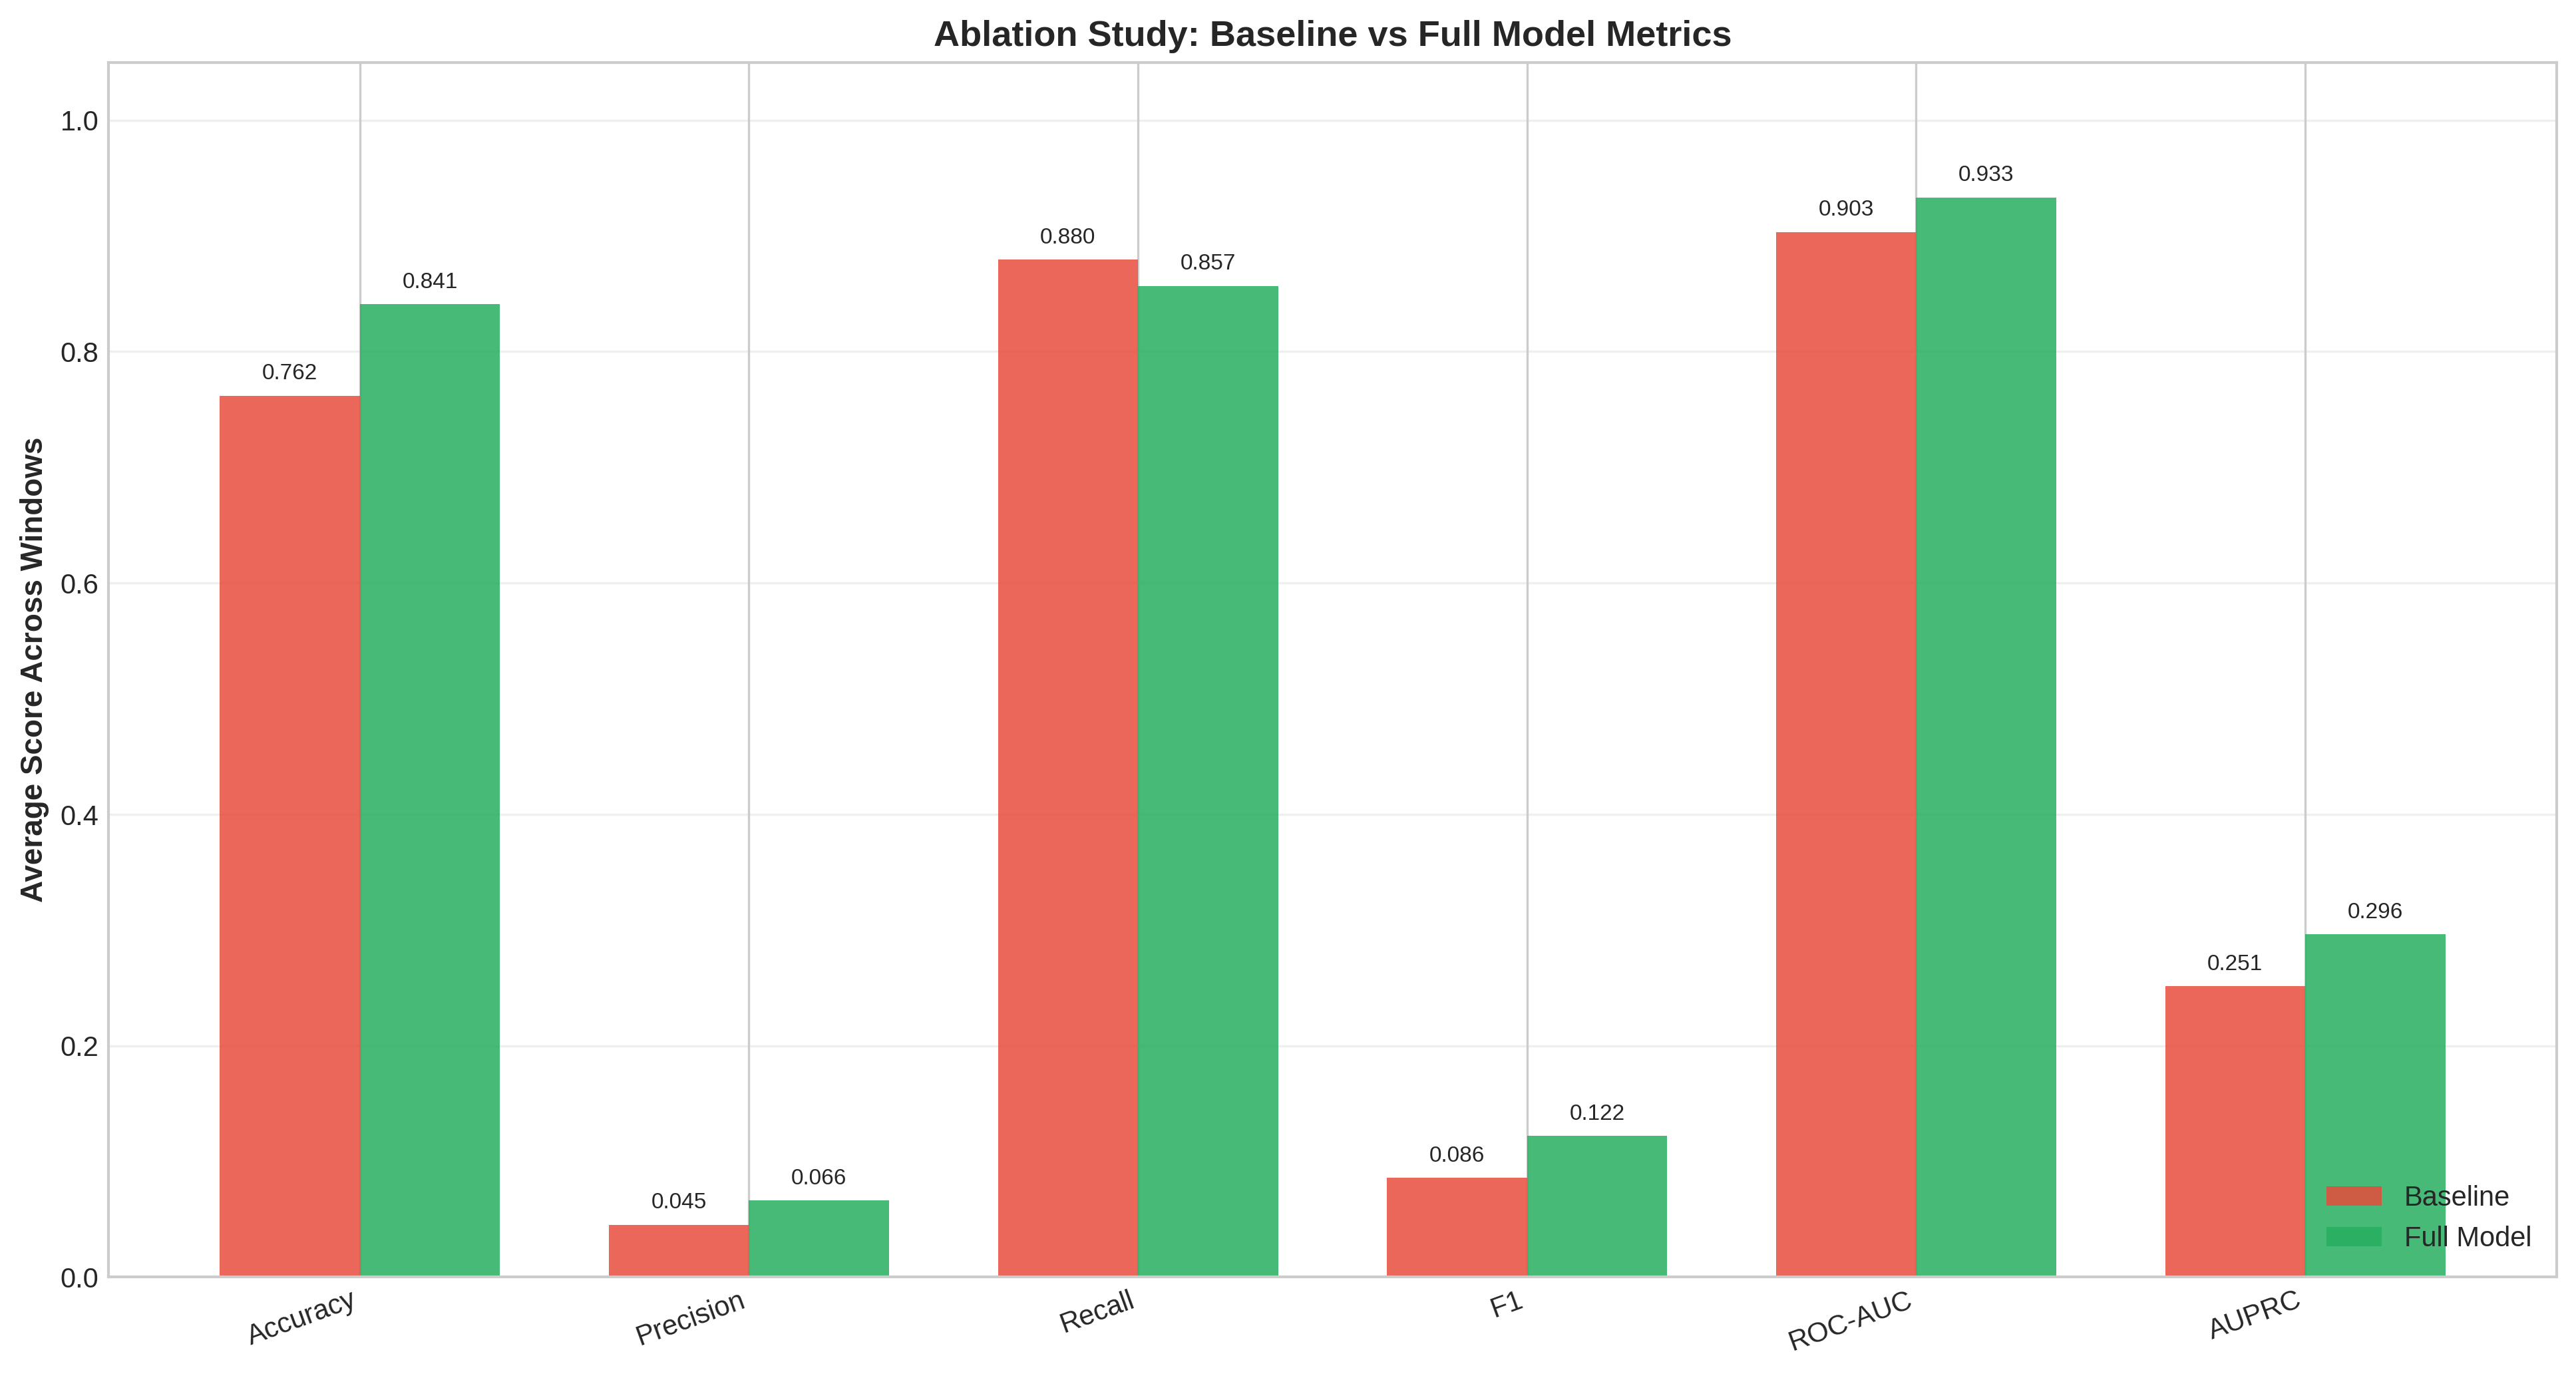
\includegraphics[width=0.95\linewidth]{imagens/HI_Small_ablation_metric_comparison.png}
    \caption{Comparação estatística das métricas de ablação (HI Small)}
    \label{fig:ablation-comparison}
\end{figure}

\subsubsection{Etapa 2: Eliminação Recursiva Guiada por SHAP}

A partir do conjunto filtrado, aplicou-se a técnica de eliminação recursiva, removendo iterativamente as \textit{features} de menor importância SHAP e monitorando a degradação de desempenho. A Tabela~\ref{tab:rfe-results} apresenta os resultados das primeiras 5 iterações.

\begin{table}{\linewidth}
    \centering
    \caption{Resultados do processo de eliminação recursiva (SHAP-RFE - HI Small)}
    \label{tab:rfe-results}
    \begin{tabular}{ccccl}
        \hline
        \textbf{Iteração} & \textbf{N Features} & \textbf{AUPRC} & \textbf{$\Delta$ AUPRC} & \textbf{Feature Removida} \\
        \hline
        0 & 33 & 0.2251 & -- & (Baseline) \\
        1 & 32 & 0.2252 & +0.0001 & \texttt{fan\_out\_count} \\
        2 & 31 & 0.2300 & +0.0049 & \texttt{cycle\_count} \\
        3 & 30 & 0.2282 & +0.0031 & \texttt{fan\_in\_count} \\
        4 & 29 & 0.2269 & +0.0019 & \texttt{local\_clustering\_coefficient} \\
        5 & 28 & 0.2204 & -0.0047 & \texttt{egonet\_density} \\
        \hline
    \end{tabular}
\end{table}

O processo identificou a iteração 2 (31 \textit{features}) como o ponto ótimo, onde o modelo alcançou AUPRC = 0.2300, representando um ganho de +2.19\% em relação ao baseline de 33 \textit{features} (AUPRC = 0.2251). A partir da iteração 5, observa-se degradação de desempenho, indicando que as \textit{features} restantes eram essenciais para a capacidade preditiva do modelo.

O conjunto final de 31 \textit{features} mantém uma composição balanceada:

\begin{itemize}
    \item \textbf{16 atributos comportamentais:} Incluindo contagens por tipo de pagamento, volumes transacionados e diversidade de moedas.
    \item \textbf{15 atributos topológicos:} Incluindo métricas de centralidade (HITS, grau, \textit{PageRank}), detecção de comunidades (Leiden) e agregação de vizinhança.
\end{itemize}

Essa redução de 36,7\% no número de \textit{features} (de 49 para 31) resulta em economias substanciais no tempo de processamento, uma vez que algoritmos como o \textit{PageRank}, \textit{Betweenness} e detecção de comunidades apresentam alta complexidade computacional em grafos de larga escala.

\begin{figure}{\linewidth}
    \centering
    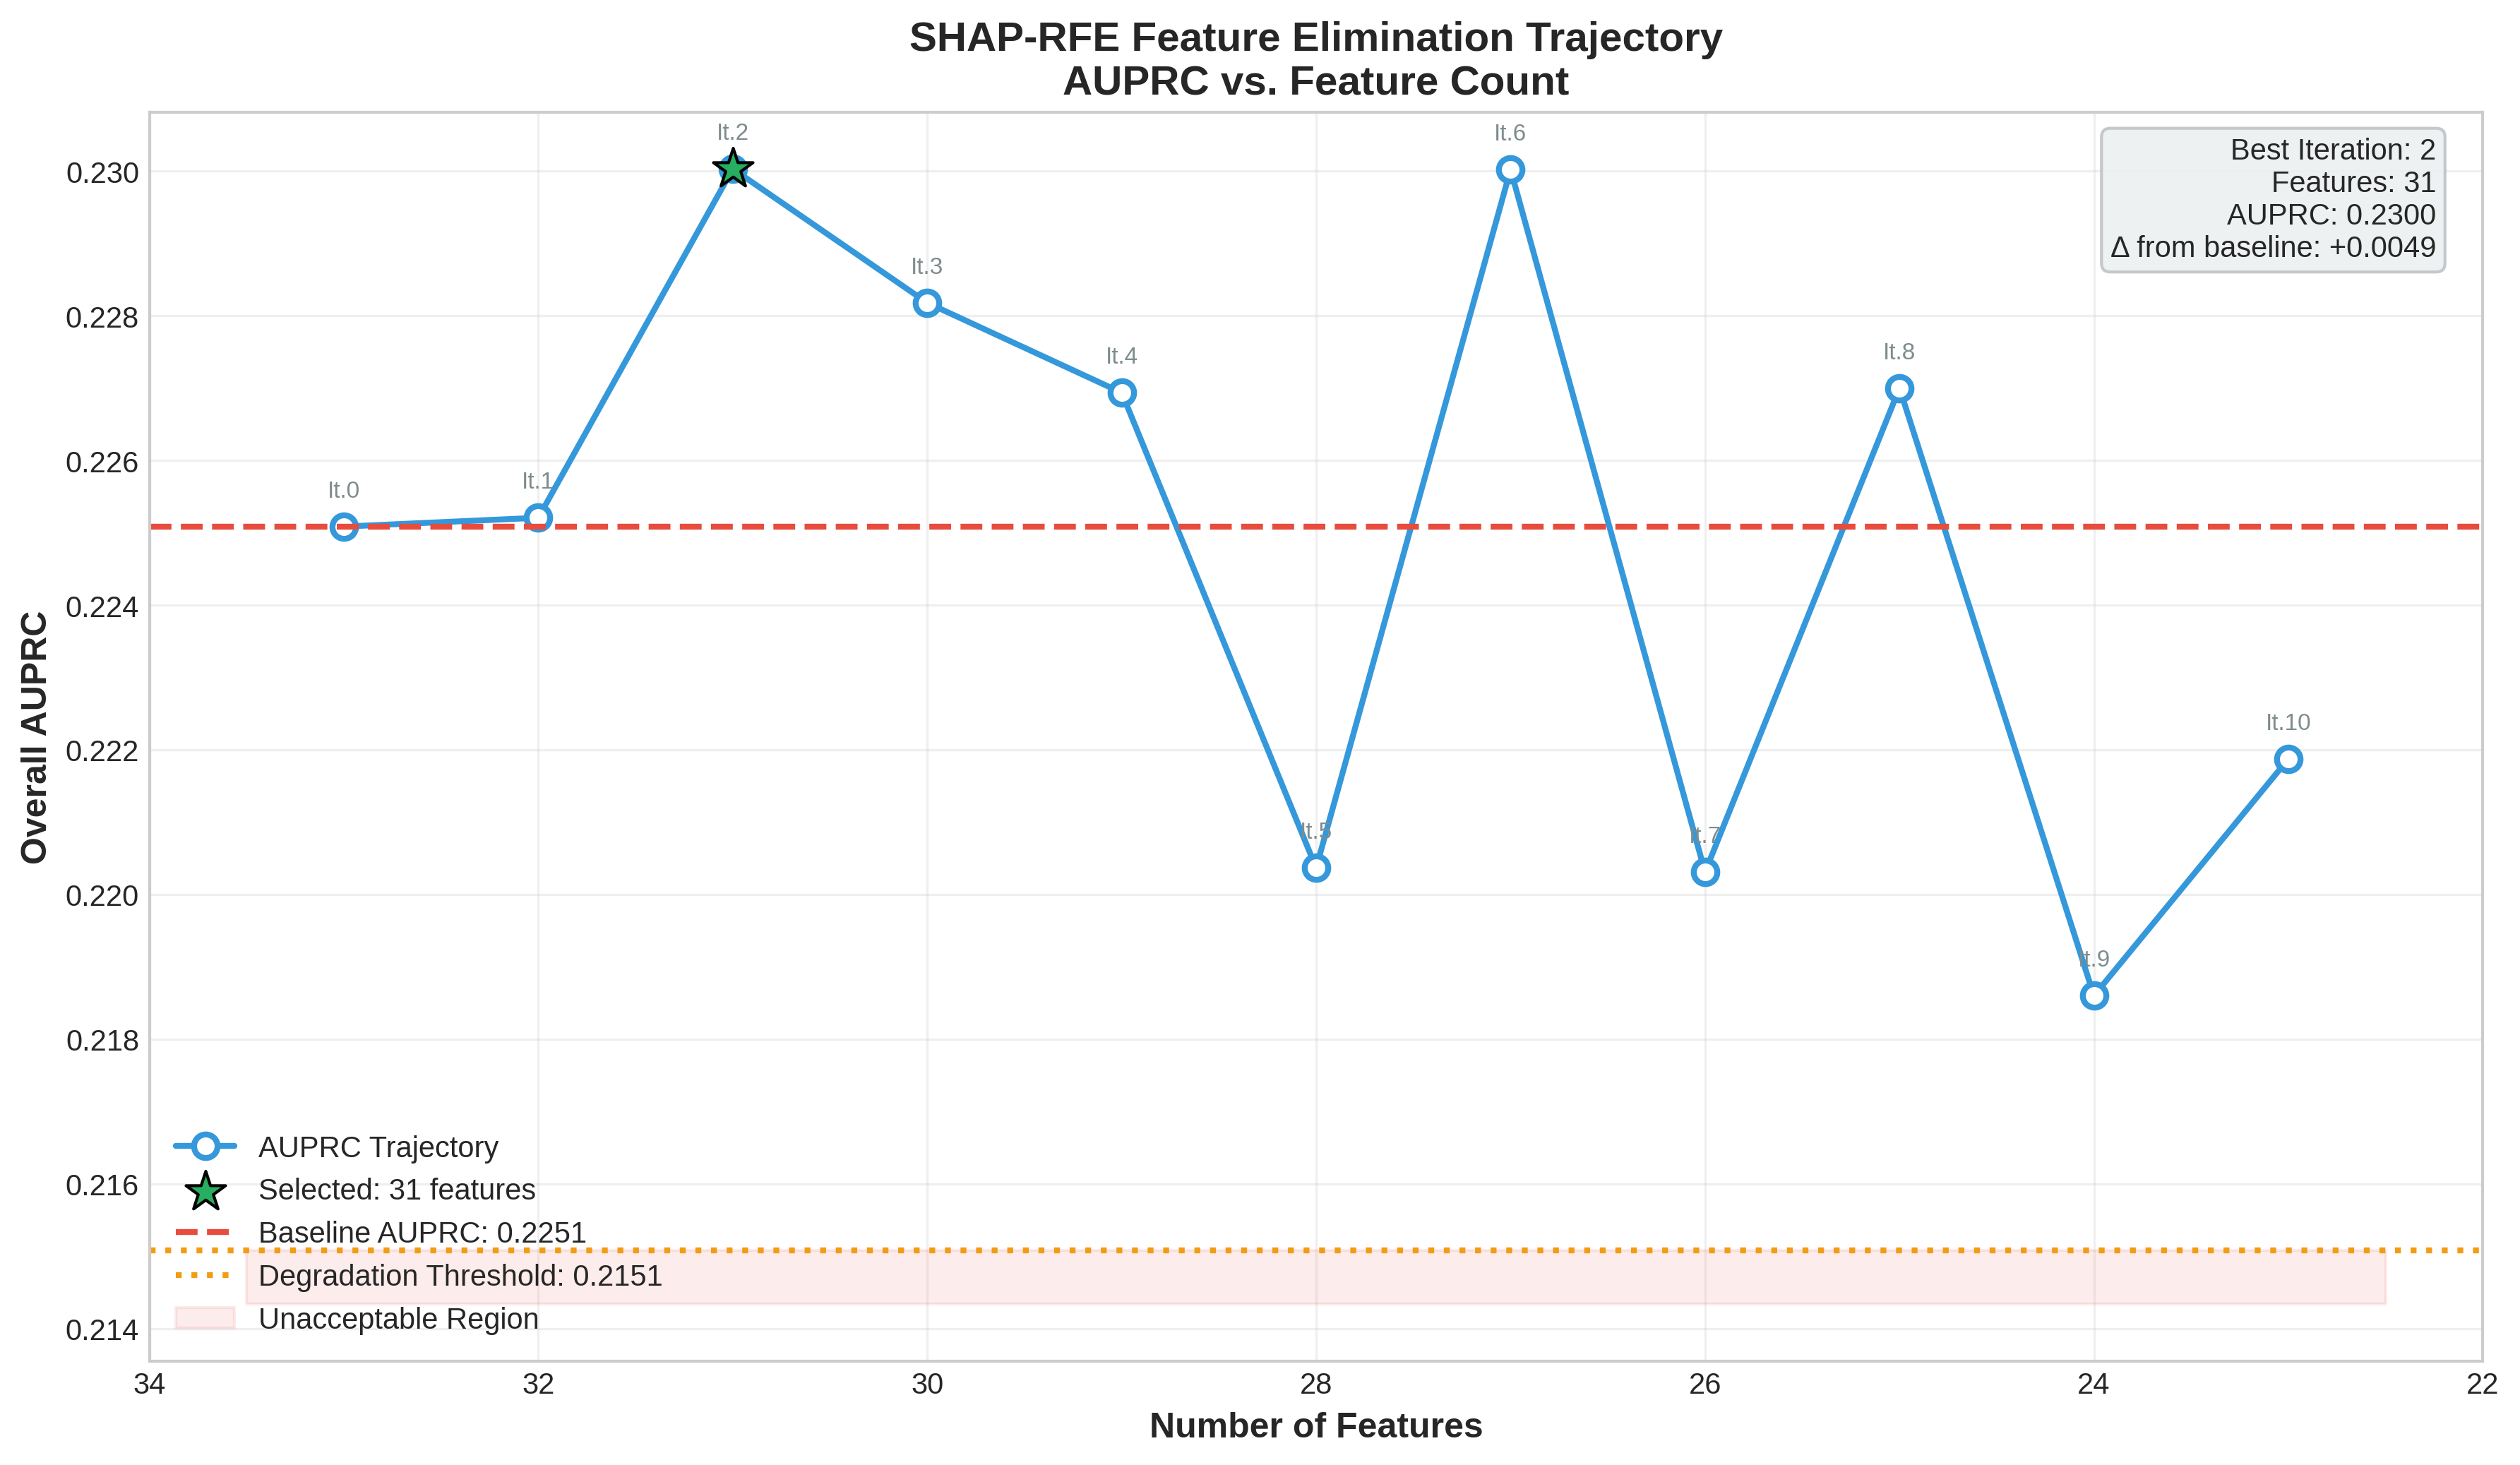
\includegraphics[width=0.95\linewidth]{imagens/HI_Small_rfe_degradation_trajectory.png}
    \caption{Trajetória de degradação durante o processo SHAP-RFE (HI Small)}
    \label{fig:rfe-trajectory}
\end{figure}

\begin{figure}{\linewidth}
    \centering
    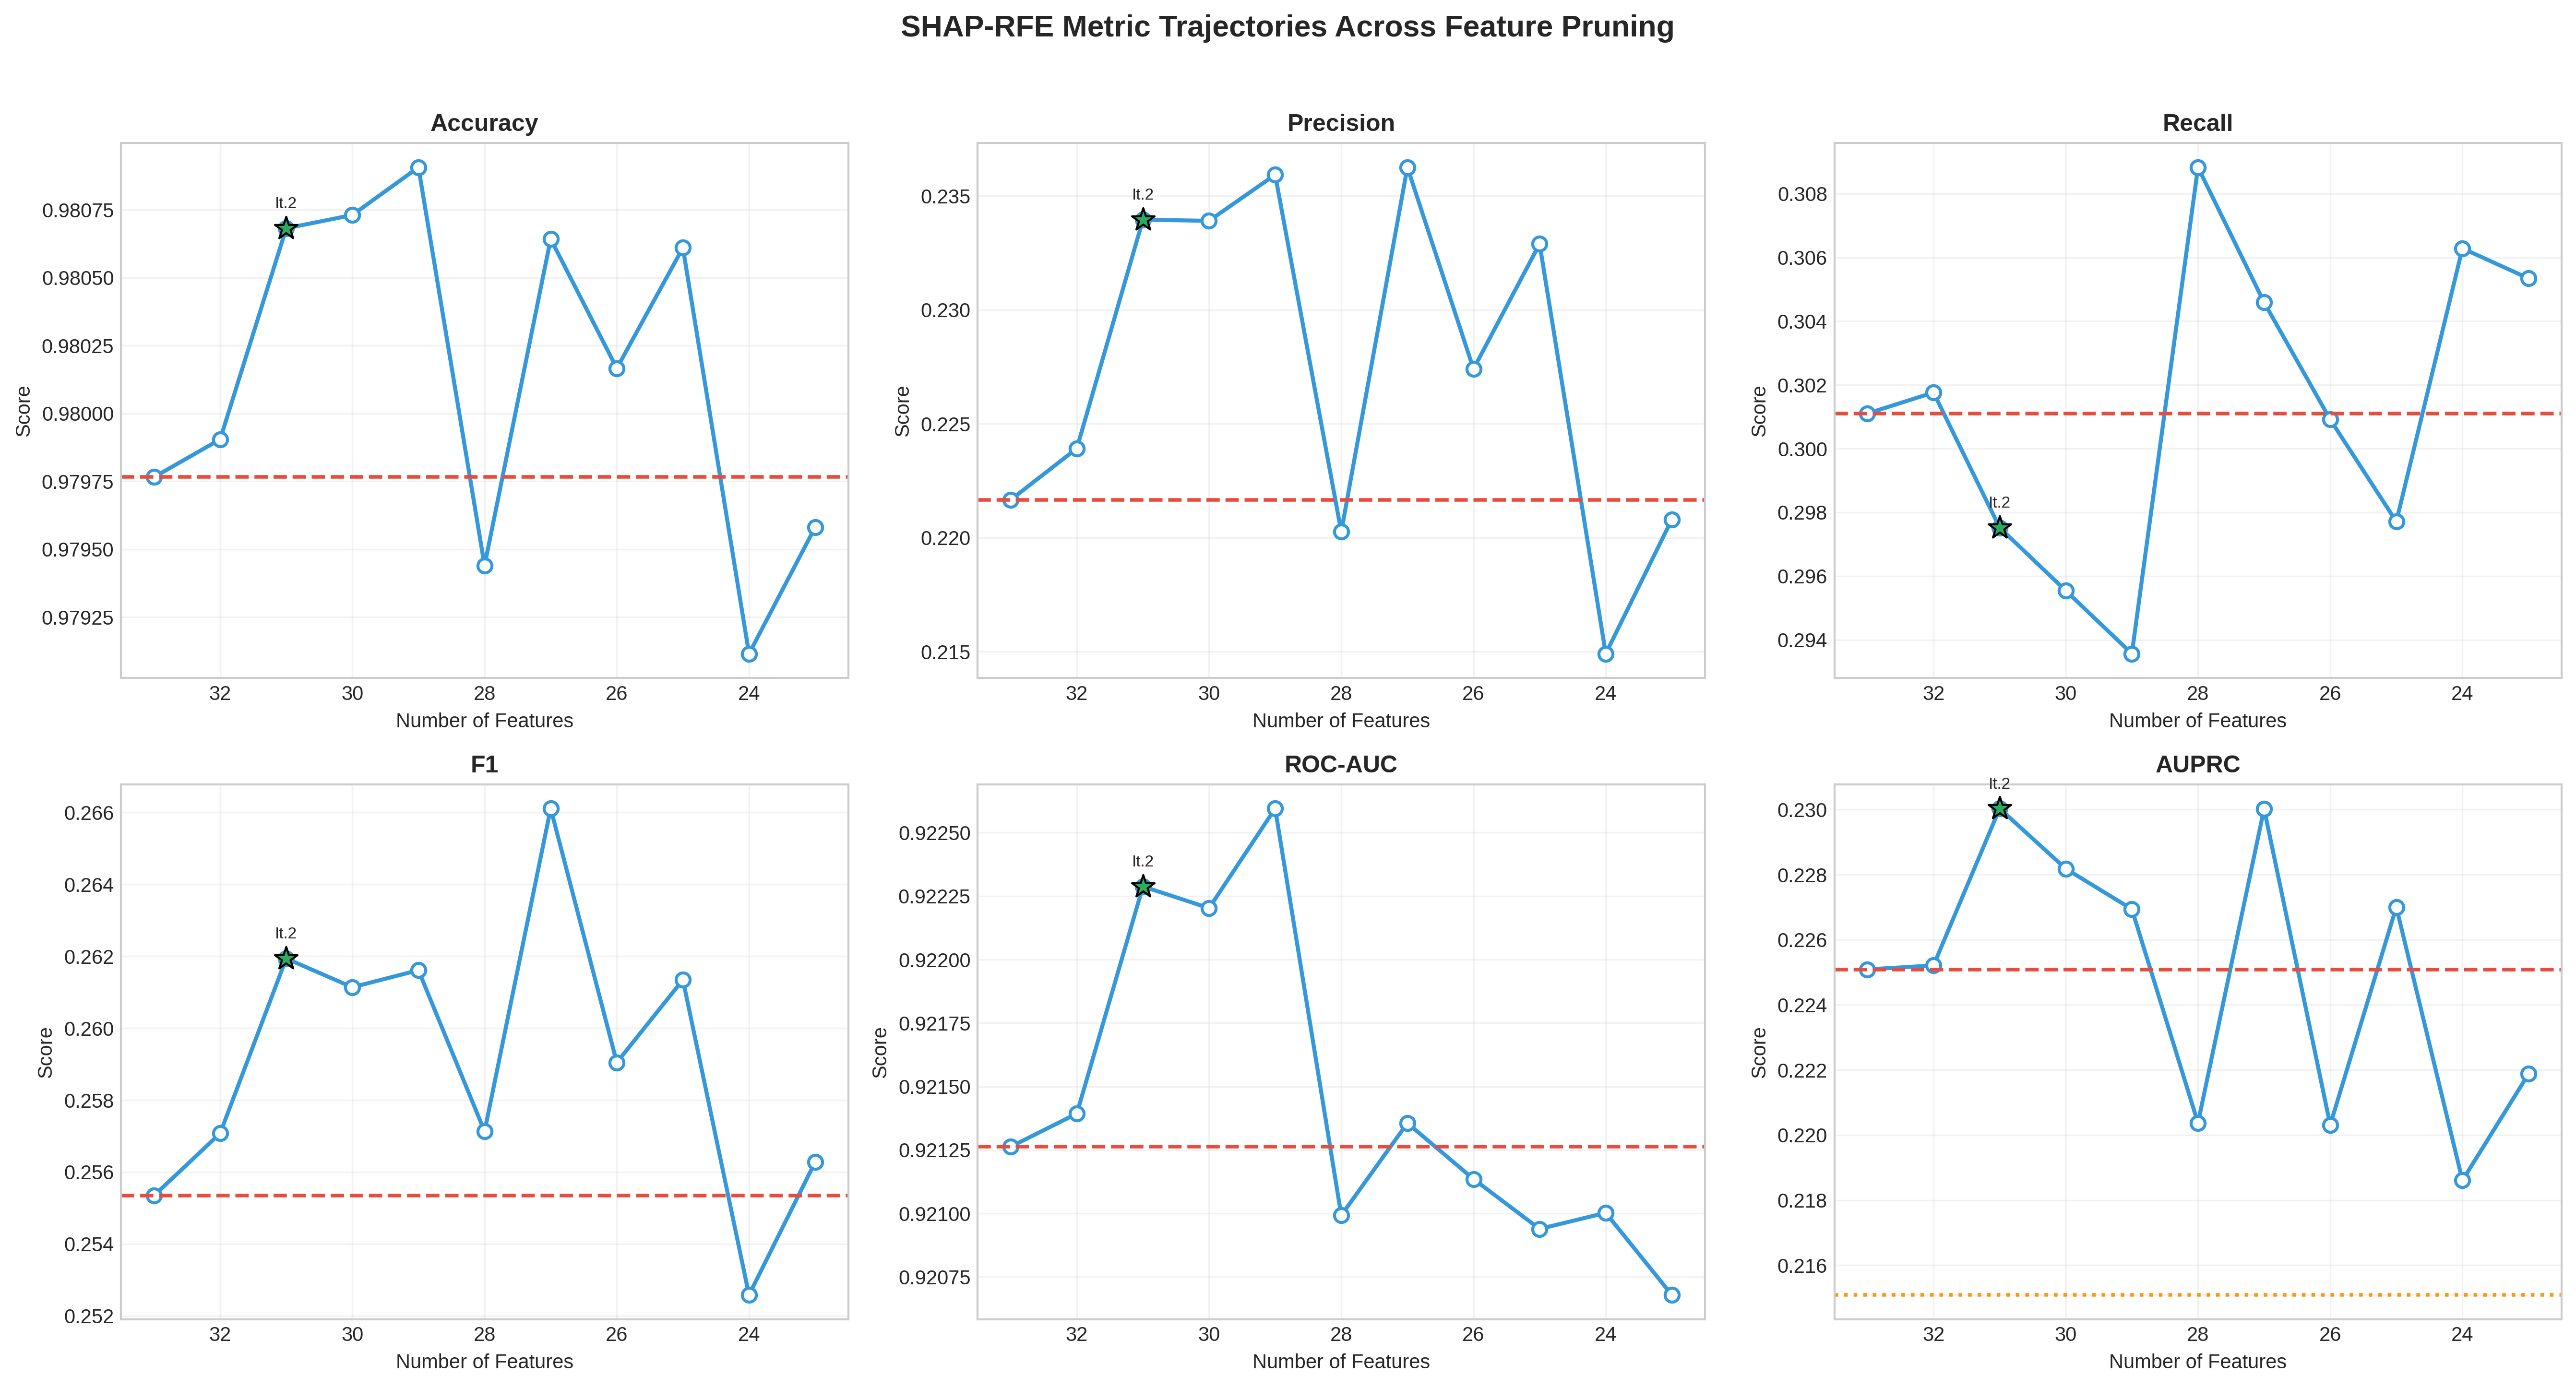
\includegraphics[width=0.95\linewidth]{imagens/HI_Small_rfe_metric_trajectories.png}
    \caption{Evolução das métricas durante o processo iterativo de eliminação de features (HI Small)}
    \label{fig:rfe-metrics}
\end{figure}

\subsection{Análise RFE no HI Medium}

Para o dataset HI Medium, o processo RFE iniciou-se com um conjunto de 30 features após o filtro de colinearidade (após remoção de 19 features redundantes). A Tabela~\ref{tab:rfe-results-medium} apresenta os resultados das iterações do RFE.

\begin{table}{\linewidth}
    \centering
    \caption{Resultados do processo de eliminação recursiva (SHAP-RFE - HI Medium)}
    \label{tab:rfe-results-medium}
    \begin{tabular}{cccc}
        \hline
        \textbf{Iteração} & \textbf{N Features} & \textbf{AUPRC} & \textbf{Status} \\
        \hline
        0 & 30 & 0.2063 & Baseline (após filtro colinearidade) \\
        1 & 29 & 0.2062 & -0.0001 \\
        2 & 28 & 0.2069 & +0.0007 \\
        3 & 27 & 0.2073 & +0.0010 \\
        4 & 26 & 0.2061 & -0.0002 \\
        5 & 25 & 0.2084 & +0.0021 \textbf{(Ótimo)} \\
        6 & 24 & 0.1991 & -0.0093 \\
        \hline
    \end{tabular}
\end{table}

O RFE no HI Medium identificou 25 features como o ponto ótimo, representando uma redução de 16.7\% em relação ao conjunto inicial de 30 (após colinearidade). O desempenho máximo de AUPRC = 0.2084 representa apenas uma pequena margem (0.2084 vs 0.2063 no baseline de 30 features), indicando que as features mais relevantes foram selecionadas. A degradação significativa após 25 features (AUPRC cai para 0.1991 com 24 features) sugere que o modelo requer pelo menos esse conjunto mínimo de atributos para discriminação eficaz.

A comparação entre os dois datasets revela um padrão interessante: embora HI Medium tenha iniciado com mais features após colinearidade (30 vs 33 no HI Small), o conjunto ótimo requer fewer features (25 vs 31). Isso sugere que a estrutura mais complexa da rede HI Medium (maior escala e conectividade) permite que informação discriminativa seja capturada com um conjunto menor e mais refinado de atributos.

\begin{figure}{\linewidth}
    \centering
    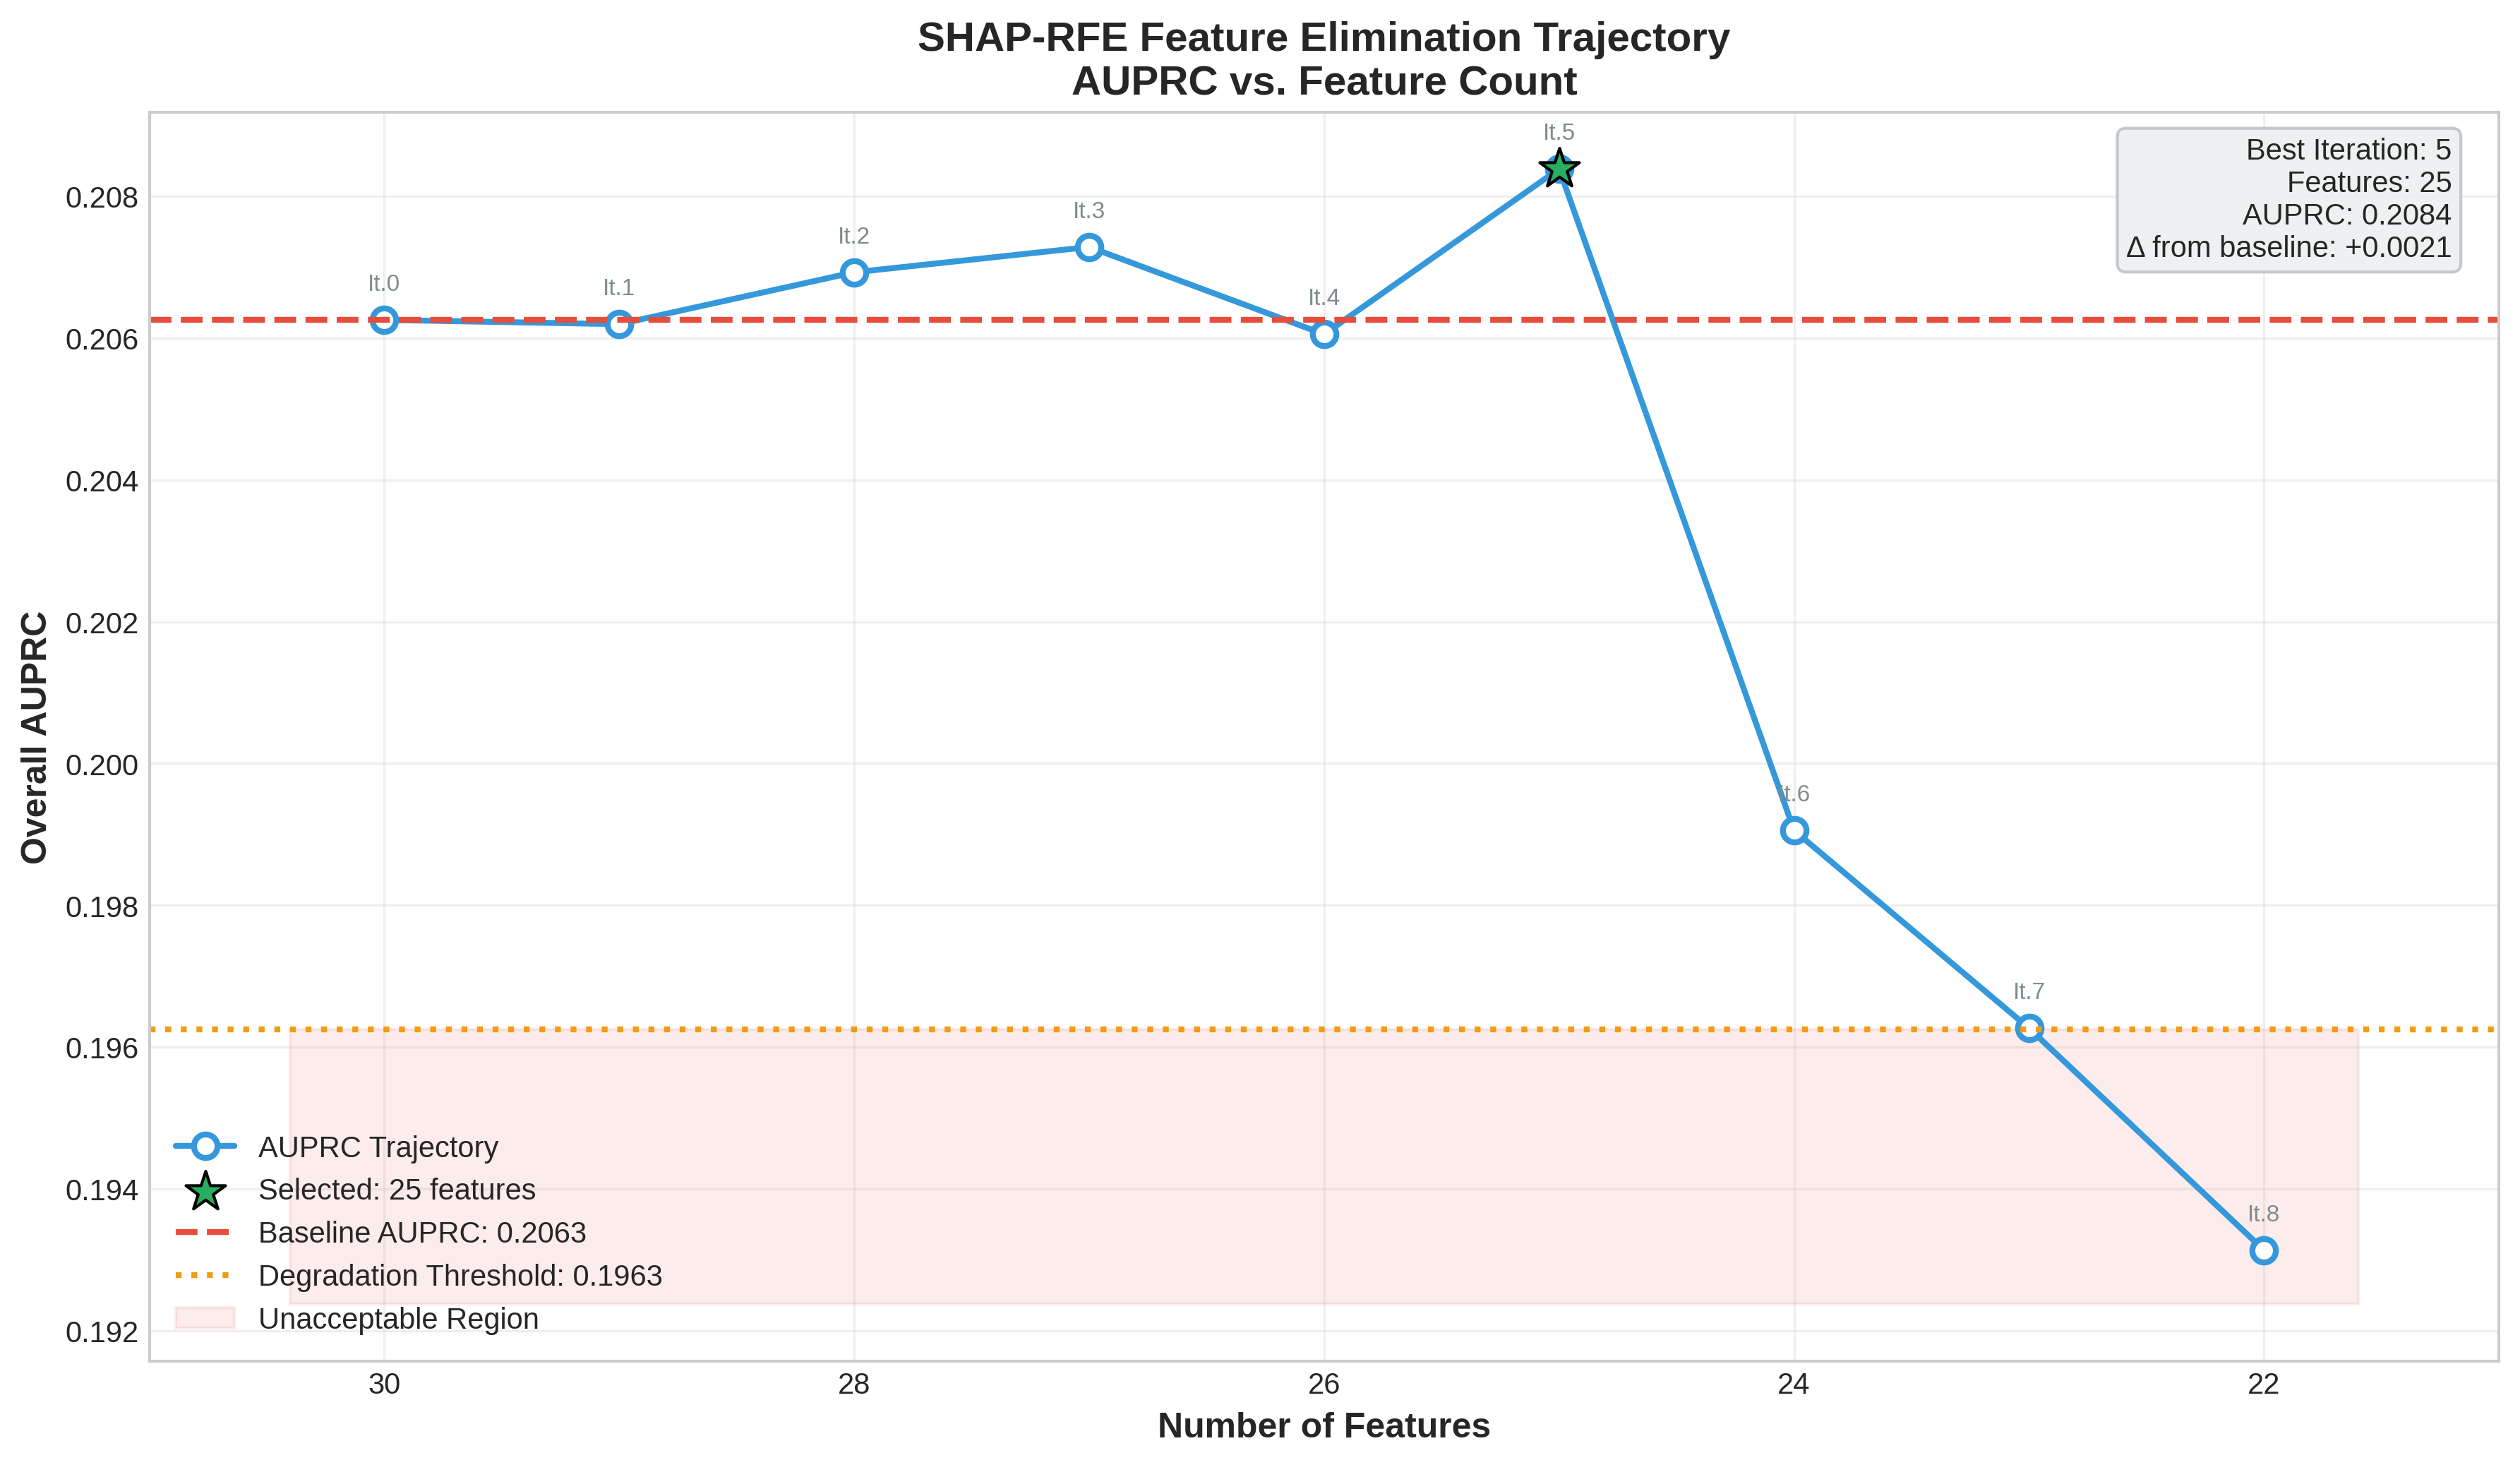
\includegraphics[width=0.95\linewidth]{imagens/HI_Medium_rfe_degradation_trajectory.png}
    \caption{Trajetória de degradação durante o processo SHAP-RFE (HI Medium)}
    \label{fig:rfe-trajectory-medium}
\end{figure}

\begin{figure}{\linewidth}
    \centering
    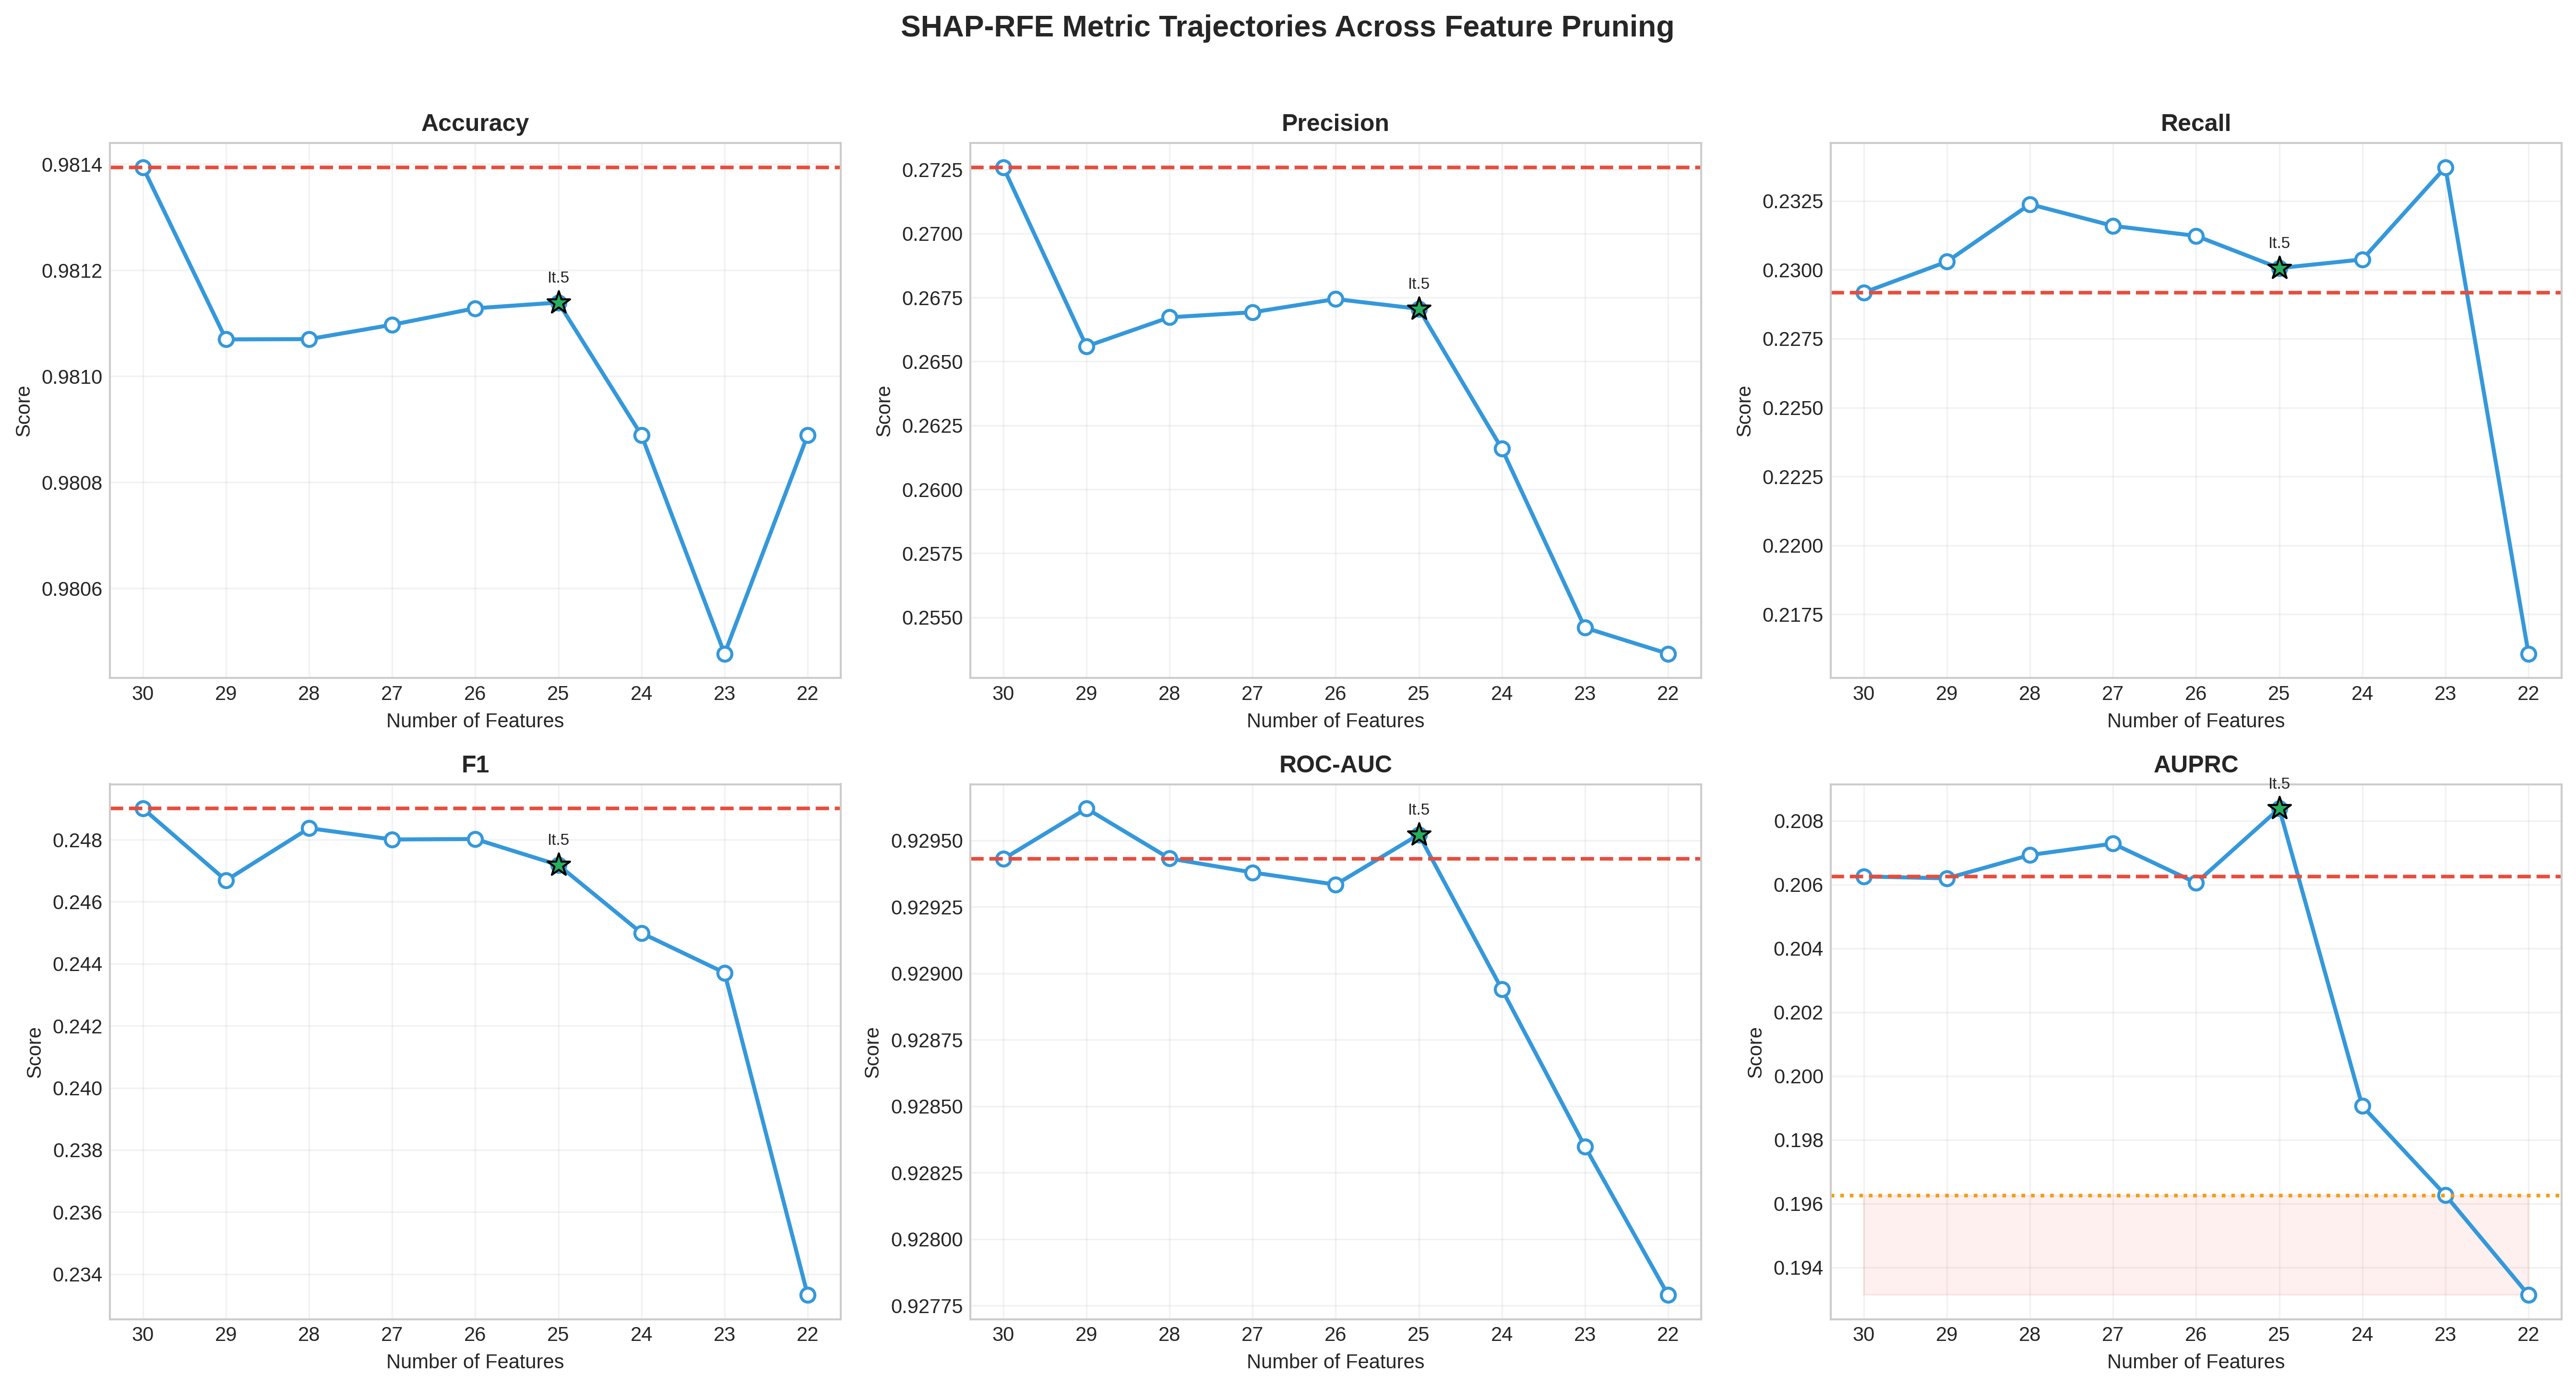
\includegraphics[width=0.95\linewidth]{imagens/HI_Medium_rfe_metric_trajectories.png}
    \caption{Evolução das métricas durante o processo iterativo de eliminação de features (HI Medium)}
    \label{fig:rfe-metrics-medium}
\end{figure}

\section{Discussão dos Resultados}

Os resultados experimentais confirmam a hipótese central deste trabalho: a incorporação de atributos topológicos extraídos de grafos temporais fornece ganhos estatisticamente significativos na detecção de esquemas de lavagem de dinheiro quando comparada a modelos baseados exclusivamente em \textit{features} comportamentais.

O ganho médio de +18\% em AUPRC, validado estatisticamente com $p = 0.0188$, demonstra que as propriedades estruturais da rede financeira carregam informação preditiva complementar que não é capturada por análises isoladas de comportamento transacional. Esse resultado alinha-se com a literatura recente, que destaca a importância de abordagens baseadas em grafos para identificar tipologias avançadas de fraude, como \textit{smurfing}, ciclos de transferência e estruturas de dispersão-concentração \cite{cheng2025graph,baigabyl2025using}.

A análise de importância via SHAP revelou que, embora as \textit{features} comportamentais tradicionais (especialmente as relacionadas a ACH e cheques) permaneçam altamente relevantes, as métricas topológicas ocupam posições de destaque no ranking de influência. Em particular, o algoritmo HITS e as métricas de grau demonstraram alta capacidade discriminativa, sugerindo que entidades fraudulentas tendem a ocupar posições estruturalmente distintas na rede: seja como pontos de concentração de fluxo (\textit{authority}) ou como nós dispersores (\textit{hub}).

A validação temporal do estudo de ablação, realizada através de \textit{forward-chaining} em 6 janelas consecutivas, confere robustez aos resultados. A consistência dos ganhos ao longo de 5 das 6 janelas indica que os padrões topológicos aprendidos pelo modelo generalizam bem para períodos futuros, um requisito crítico para a implantação em ambientes de produção.

\begin{figure}{\linewidth}
    \centering
    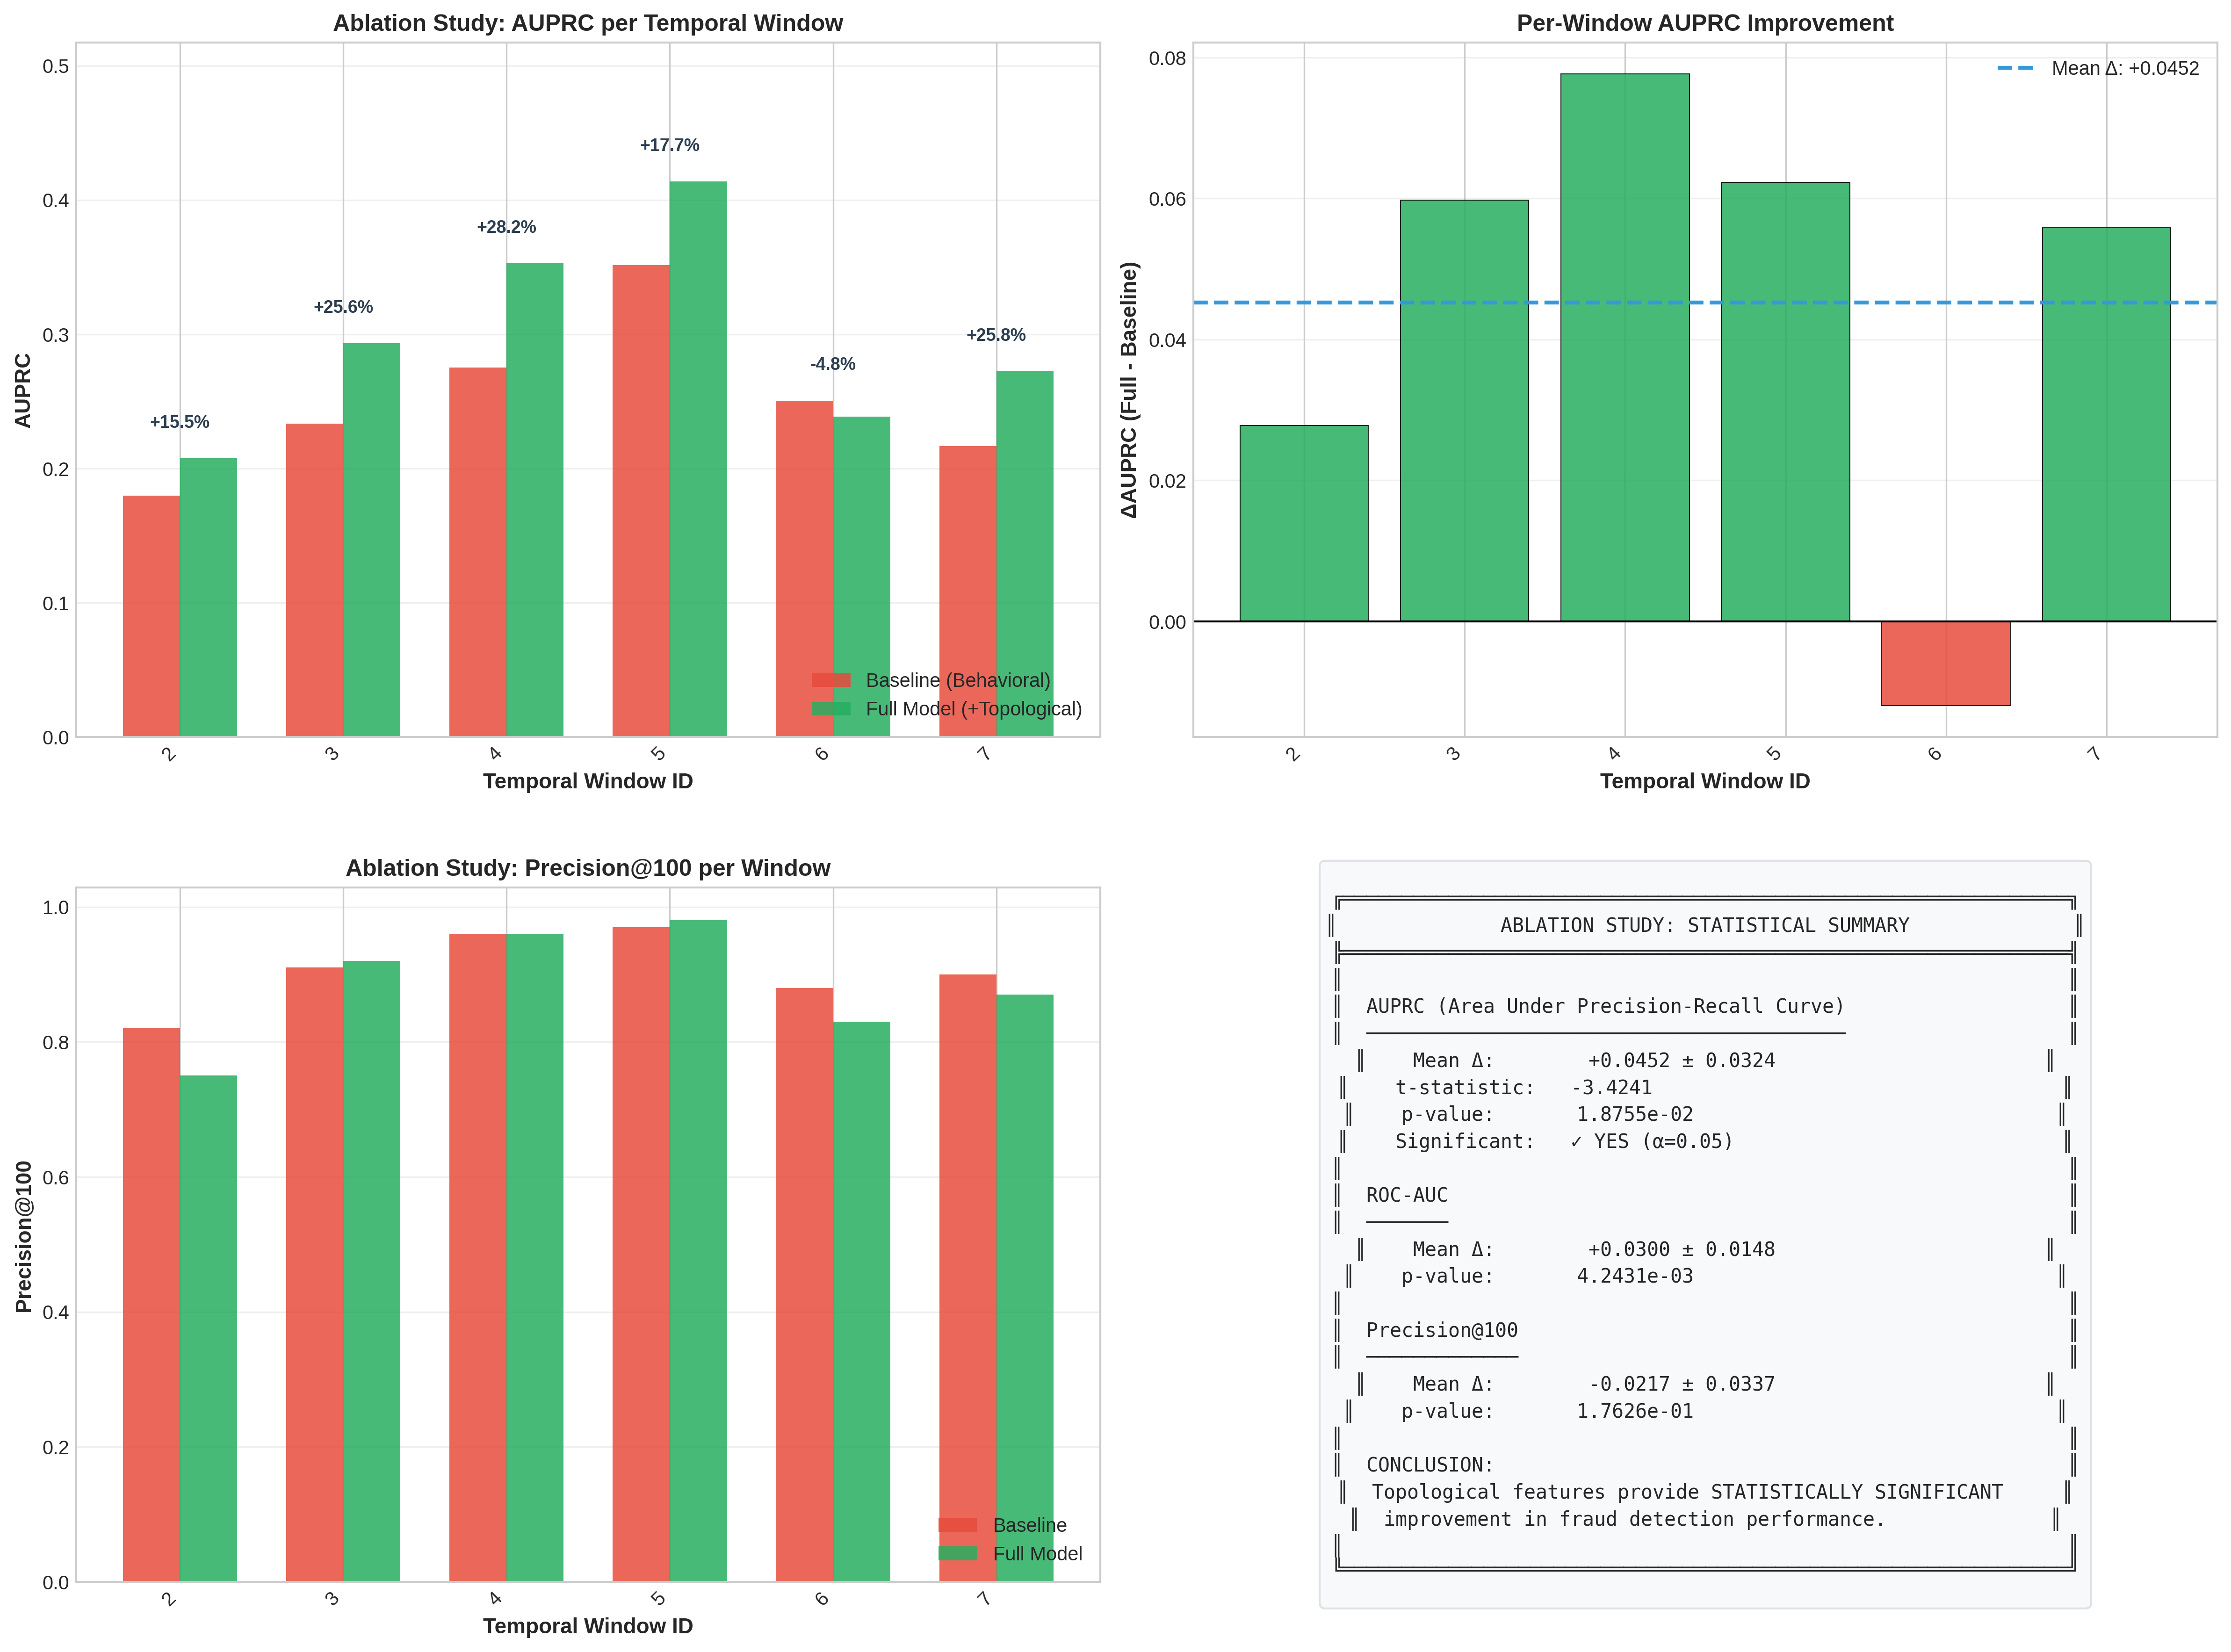
\includegraphics[width=0.95\linewidth]{imagens/HI_Small_ablation_lift.png}
    \caption{Lift percentual por janela temporal e métrica de avaliação (HI Small)}
    \label{fig:ablation-lift}
\end{figure}

\begin{figure}{\linewidth}
    \centering
    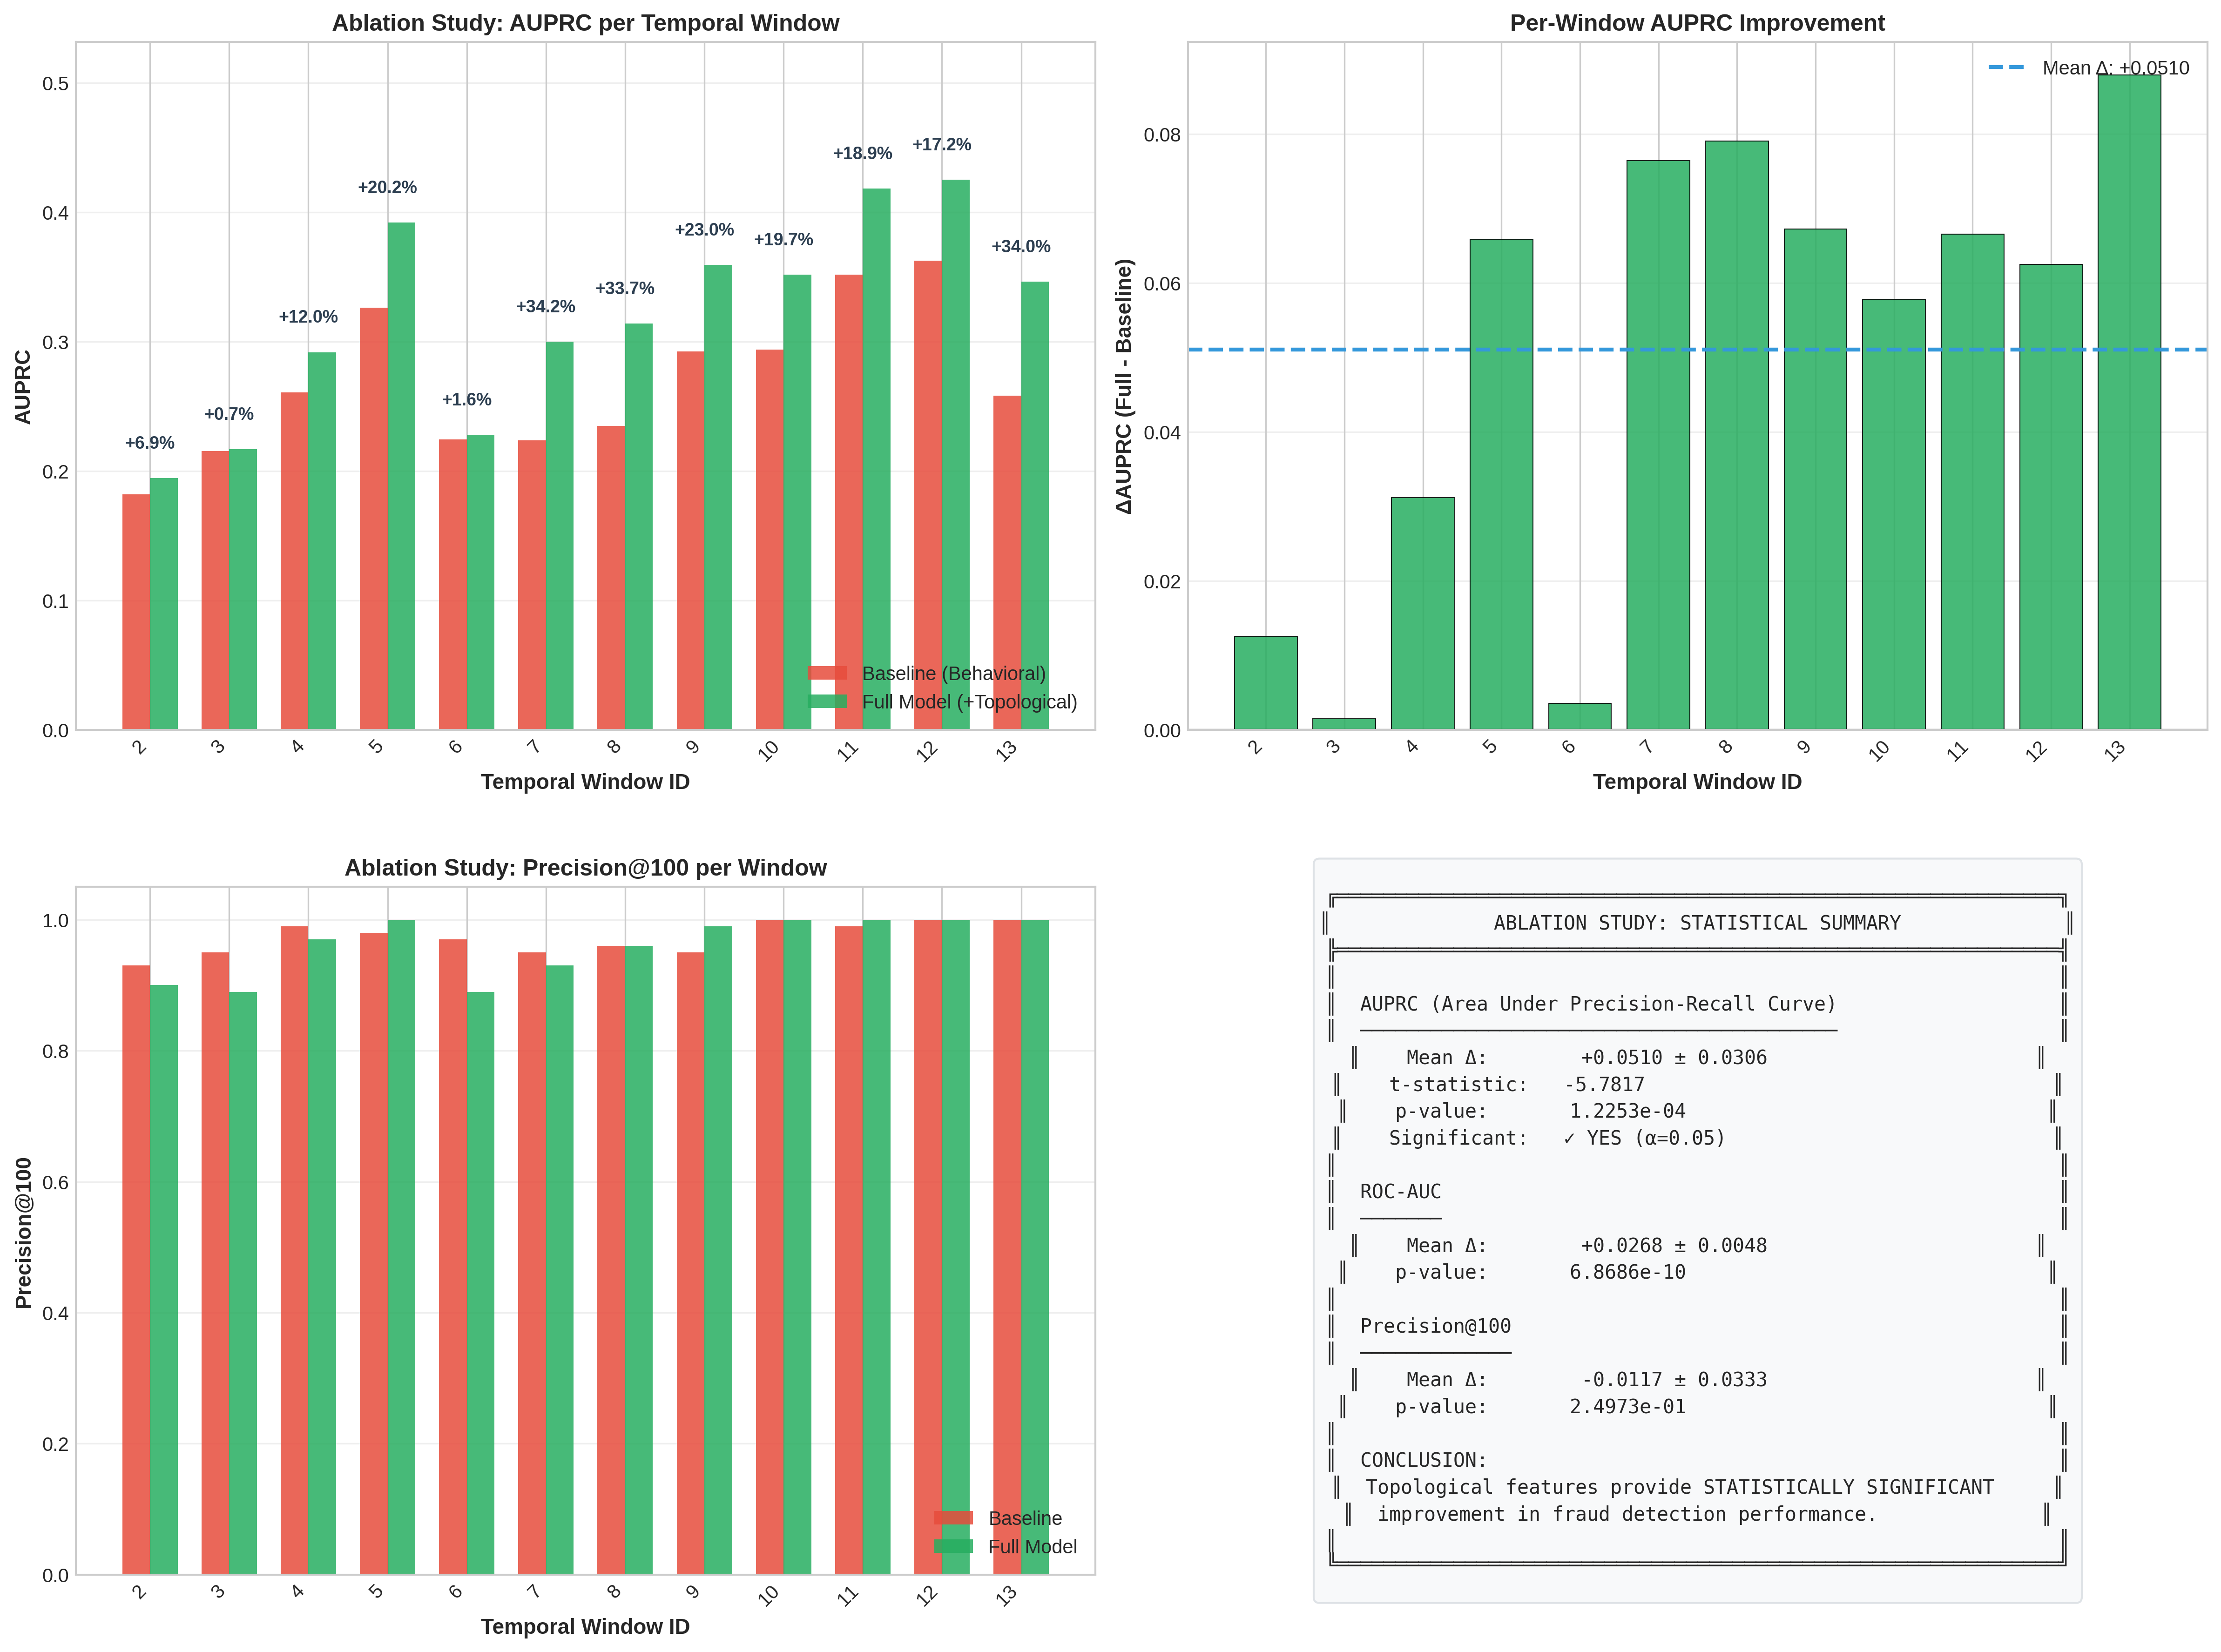
\includegraphics[width=0.95\linewidth]{imagens/HI_Medium_ablation_lift.png}
    \caption{Lift percentual por janela temporal e métrica de avaliação (HI Medium)}
    \label{fig:ablation-lift-medium}
\end{figure}

Por outro lado, a redução observada no \textit{Recall} geral (HI Small: -2.58%, HI Medium: -2.00%) e as oscilações nas métricas P@100 e P@200 evidenciam um \textit{trade-off} inerente: ao refinar a fronteira de decisão para minimizar falsos positivos, o modelo torna-se mais conservador em algumas situações, potencialmente deixando de capturar fraudes de baixa sinalização topológica. Esse comportamento é esperado e aceitável no contexto operacional de \textit{compliance}, onde a priorização de alertas de alta confiança reduz a sobrecarga investigativa, mesmo que isso implique em uma pequena perda marginal de cobertura total.

A otimização do conjunto de \textit{features} via SHAP-RFE demonstrou que é possível reduzir significativamente o número de atributos topológicos sem comprometer o desempenho preditivo: 36,7\% no HI Small (de 49 para 31) e 16,7\% no HI Medium (de 30 para 25). Esse resultado possui implicações práticas significativas: a extração de métricas como \textit{Betweenness Centrality} e detecção de comunidades em grafos de milhões de nós é computacionalmente custosa. Ao identificar um subconjunto eficiente de atributos topológicos essenciais (15-16 features topológicos em ambos os datasets), o sistema torna-se viável para operação em infraestruturas com recursos limitados, expandindo sua aplicabilidade a instituições financeiras de médio porte que não dispõem de clusters computacionais de alta capacidade.

\chapter{Conclusão}

Este trabalho investigou a contribuição de atributos topológicos extraídos de grafos temporais para a detecção de esquemas de lavagem de dinheiro utilizando algoritmos de \textit{Gradient Boosting}. Através de um estudo de ablação controlado e estatisticamente validado, demonstrou-se que a incorporação de \textit{features} estruturais de rede resulta em ganhos significativos de desempenho em relação a modelos baseados exclusivamente em atributos comportamentais.

\section{Principais Contribuições}

Os resultados obtidos confirmam as hipóteses centrais do trabalho e fornecem evidências quantitativas para as seguintes contribuições:

\begin{enumerate}
    \item \textbf{Validação empírica do ganho topológico:} O modelo completo (comportamental + topológico) alcançou AUPRC média de 0.2965, representando um ganho estatisticamente significativo de +18.00\% ($p = 0.0188$) em relação ao modelo de base (AUPRC = 0.2513). Ganhos similares foram observados em precisão (+42.80\%, $p = 0.0070$), F1-Score (+39.81\%, $p = 0.0055$) e ROC-AUC (+3.32\%, $p = 0.0042$).
    
    \item \textbf{Identificação de \textit{features} topológicas críticas:} A análise SHAP revelou que métricas de centralidade (HITS, grau, \textit{PageRank}), detecção de comunidades (Leiden) e agregação de vizinhança ocupam posições de destaque no ranking de importância preditiva, demonstrando que entidades fraudulentas exibem assinaturas estruturais distintas na rede financeira.
    
    \item \textbf{Otimização para implantação operacional:} Através de um processo em dois estágios (filtro de colinearidade + SHAP-RFE), identificou-se um subconjunto eficiente de 31 \textit{features} (redução de 36.7\%) que mantém desempenho superior ao modelo de base original, viabilizando a implantação em ambientes com recursos computacionais limitados.
    
    \item \textbf{Robustez temporal:} A validação via \textit{forward-chaining} em 6 janelas temporais demonstrou consistência dos ganhos ao longo do tempo, indicando que os padrões topológicos aprendidos generalizam para períodos futuros, um requisito essencial para sistemas de detecção de fraudes em produção.
\end{enumerate}

\section{Implicações Práticas}

Do ponto de vista operacional, os resultados possuem implicações diretas para equipes de \textit{compliance} de instituições financeiras:

\begin{itemize}
    \item \textbf{Redução de falsos positivos:} O ganho de +42.80\% em precisão implica em uma redução substancial de alertas falsos, diminuindo a sobrecarga investigativa e permitindo que analistas foquem em casos de alto risco real.
    
    \item \textbf{Captura incremental de fraudes:} O modelo completo identificou 29 entidades fraudulentas adicionais (0.80\% de melhoria relativa), demonstrando que as \textit{features} topológicas capturam padrões estruturais que escapam à análise comportamental isolada.
    
    \item \textbf{Viabilidade computacional:} A redução do conjunto de \textit{features} de 49 para 31 atributos, sem perda de desempenho, torna o sistema viável para operação em infraestruturas de médio porte, expandindo sua aplicabilidade além de grandes instituições bancárias.
\end{itemize}

\section{Limitações e Trabalhos Futuros}

Embora os resultados sejam promissores, o estudo apresenta limitações que devem ser consideradas:

\begin{enumerate}
    \item \textbf{Uso de dados sintéticos:} A validação foi realizada exclusivamente sobre o \textit{dataset} AMLworld, que, apesar de sua fidelidade estrutural, não captura toda a complexidade e diversidade de padrões observados em transações bancárias reais. A aplicação do sistema a dados reais de instituições financeiras é um próximo passo essencial.
    
    \item \textbf{Escala computacional:} Embora a otimização via SHAP-RFE tenha reduzido o custo de extração de \textit{features}, o processamento de grafos com milhões de nós ainda exige recursos significativos. Investigações futuras devem explorar técnicas de amostragem de grafos e aproximações algorítmicas para viabilizar a operação em tempo real.
    
    \item \textbf{Evolução temporal dos padrões:} Fraudadores adaptam suas estratégias ao longo do tempo. Trabalhos futuros devem investigar mecanismos de retreinamento contínuo e detecção de \textit{concept drift} para manter a eficácia do sistema em cenários de evolução adversarial.
    
    \item \textbf{Explicabilidade para auditoria regulatória:} Embora a técnica SHAP forneça interpretabilidade a nível de \textit{feature}, a justificação de alertas individuais para fins de auditoria regulatória exige métodos de explicação a nível de instância. A integração de técnicas como LIME (\textit{Local Interpretable Model-agnostic Explanations}) e caminhos de ativação em grafos pode fortalecer a rastreabilidade das decisões do modelo.
\end{enumerate}

\section{Considerações Finais}

Este trabalho demonstrou que a modelagem de redes financeiras como grafos temporais e a extração de atributos topológicos fornecem ganhos mensuráveis e estatisticamente validados para a detecção de lavagem de dinheiro. A integração de Ciência de Dados de Grafos com algoritmos de \textit{Gradient Boosting} representa uma abordagem promissora para sistemas de \textit{Anti-Money Laundering}, capaz de capturar tanto o comportamento individual das entidades quanto as propriedades estruturais das redes de transações.

Os resultados reforçam a importância de abordagens multimodais que combinam sinais comportamentais e topológicos, especialmente em cenários onde fraudadores utilizam estratégias sofisticadas de ofuscação, como \textit{smurfing}, ciclos de transferência e estruturas de dispersão-concentração. À medida que os esquemas de lavagem de dinheiro tornam-se cada vez mais complexos e distribuídos, a incorporação de técnicas baseadas em grafos deixa de ser opcional e torna-se um requisito fundamental para a eficácia dos sistemas de detecção de fraudes financeiras.


\bibliography{bibliografia,exemplos,abnt-options}

\end{document}
